% ═══════════════════════════════════════════════════════════════════════════════
% DEEP DATA ANALYSIS REPORT — Aerospace Structural Design Dataset
% Prepared for L&T Technology Services
% ═══════════════════════════════════════════════════════════════════════════════
\documentclass[11pt, a4paper]{report}

% ── Packages ──────────────────────────────────────────────────────────────────
\usepackage[utf8]{inputenc}
\usepackage[T1]{fontenc}
\usepackage{lmodern}
\usepackage[margin=2.2cm, top=2.5cm, bottom=2.5cm]{geometry}
\usepackage{graphicx}
\usepackage{booktabs}
\usepackage{longtable}
\usepackage{array}
\usepackage{xcolor}
\usepackage{hyperref}
\usepackage{fancyhdr}
\usepackage{titlesec}
\usepackage{caption}
\usepackage{subcaption}
\usepackage{amsmath, amssymb}
\usepackage{multirow}
\usepackage{enumitem}
\usepackage{float}
\usepackage[most]{tcolorbox}
\usepackage{colortbl}
\usepackage{tabularx}
\usepackage{setspace}
\usepackage{pdfpages}

% ── Colors ────────────────────────────────────────────────────────────────────
\definecolor{navy}{HTML}{1B2A4A}
\definecolor{teal}{HTML}{2EC4B6}
\definecolor{coral}{HTML}{E07A5F}
\definecolor{gold}{HTML}{F2CC8F}
\definecolor{lightbg}{HTML}{F7F9FC}
\definecolor{slate}{HTML}{6C7A89}

% ── Styling ───────────────────────────────────────────────────────────────────
\hypersetup{colorlinks=true, linkcolor=navy, urlcolor=teal, citecolor=coral}
\setlength{\parindent}{0pt}
\setlength{\parskip}{6pt}
\onehalfspacing

% Headers and footers
\pagestyle{fancy}
\fancyhf{}
\fancyhead[L]{\footnotesize\textcolor{slate}{Deep Data Analysis Report}}
\fancyhead[R]{\footnotesize\textcolor{slate}{Aerospace Structural Design}}
\fancyfoot[C]{\thepage}
\renewcommand{\headrulewidth}{0.4pt}

% Chapter/section styling
\titleformat{\chapter}[display]
  {\normalfont\huge\bfseries\color{navy}}
  {\chaptertitlename\ \thechapter}{16pt}{\Huge}
\titlespacing*{\chapter}{0pt}{-20pt}{20pt}

\titleformat{\section}{\large\bfseries\color{navy}}{{\thesection}}{1em}{}
\titleformat{\subsection}{\normalsize\bfseries\color{navy!80}}{{\thesubsection}}{1em}{}

% Custom boxes
\newtcolorbox{findingbox}{
  colback=lightbg, colframe=teal, boxrule=0.8pt,
  arc=3pt, left=8pt, right=8pt, top=6pt, bottom=6pt,
  title={\textbf{Key Finding}}, fonttitle=\color{navy}\bfseries
}
\newtcolorbox{warningbox}{
  colback=coral!5, colframe=coral, boxrule=0.8pt,
  arc=3pt, left=8pt, right=8pt, top=6pt, bottom=6pt,
  title={\textbf{Red Line}}, fonttitle=\color{coral!80!black}\bfseries
}
\newtcolorbox{insightbox}[1][]{
  colback=lightbg, colframe=navy, boxrule=0.5pt,
  arc=3pt, left=8pt, right=8pt, top=6pt, bottom=6pt, #1
}

% ── Graphics path ─────────────────────────────────────────────────────────────
\graphicspath{{plots/}}

% ══════════════════════════════════════════════════════════════════════════════
\begin{document}

% ── Title Page ────────────────────────────────────────────────────────────────
\begin{titlepage}
\begin{center}
\vspace*{2cm}

{\Huge\bfseries\textcolor{navy}{Deep Data Analysis Report}}\\[0.8cm]
{\Large\textcolor{slate}{Aerospace Structural Design Dataset}}\\[0.3cm]
{\large\textcolor{slate}{Comprehensive Statistical \& Domain Analysis}}

\vspace{1.5cm}

\rule{0.6\textwidth}{1.5pt}\\[0.5cm]

{\large
\begin{tabular}{rl}
\textbf{Dataset:} & Aerospace Structural Design (300 rows $\times$ 22 features) \\[4pt]
\textbf{Domain:} & Quantum-Optimized Structural Engineering \\[4pt]
\textbf{Scope:} & Full univariate, multivariate, domain, \& anomaly analysis \\[4pt]
\textbf{Figures:} & 27 publication-quality visualizations \\[4pt]
\textbf{Date:} & March 2026 \\
\end{tabular}
}

\vspace{1.5cm}
\rule{0.6\textwidth}{1.5pt}

\vspace{2cm}

{\large Prepared for}\\[0.3cm]
{\Large\bfseries L\&T Technology Services}\\[1cm]

{\footnotesize\textcolor{slate}{This document is confidential and intended solely for the recipient.}}
\end{center}
\end{titlepage}

% ── Table of Contents ─────────────────────────────────────────────────────────
\tableofcontents
\newpage

% ══════════════════════════════════════════════════════════════════════════════
\chapter{Executive Summary}
% ══════════════════════════════════════════════════════════════════════════════

This report presents a comprehensive statistical and domain-informed analysis of the \textbf{Aerospace Structural Design Dataset}, a 300-row, 22-feature tabular dataset capturing the intersection of material science, flight environment simulation, structural geometry, and quantum-inspired optimization for aerospace applications.

\section{Dataset at a Glance}

\begin{insightbox}
\begin{tabularx}{\textwidth}{lX}
\textbf{Rows:} & 300 (zero nulls, zero duplicates, 100\% complete) \\
\textbf{Numeric features:} & 14 (continuous material, environmental, and geometric properties) \\
\textbf{Categorical features:} & 8 (material type, structural shape, optimization algorithm, 4 targets) \\
\textbf{Target variables:} & 4 multi-class: Vibration Damping, Computational Time, Weight Efficiency, Durability \\
\textbf{Unique aspect:} & Quantum algorithm optimization (Chaotic Quantum Genetic + Shark Optimizer) \\
\end{tabularx}
\end{insightbox}

\section{Principal Findings}

\begin{enumerate}[leftmargin=*, itemsep=4pt]
\item \textbf{Uniform-like distributions.} All 14 numeric features follow platykurtic distributions (kurtosis $\approx -1.1$ to $-1.35$) with near-zero skewness. Shapiro--Wilk tests reject normality for every feature ($p < 10^{-5}$). This is consistent with a simulation-generated dataset sampling uniformly across a defined design space.

\item \textbf{Tri-modal material structure.} The Elastic Modulus $E$ spans 50--200~GPa, naturally partitioning into three regimes: Aluminum ($\sim$50--100), Titanium ($\sim$100--150), and Carbon Fiber ($\sim$150--200). This tri-modal structure is the single most important distributional feature for any synthetic data generator to capture.

\item \textbf{ISA non-compliance.} Temperature and Pressure do \emph{not} follow the International Standard Atmosphere (ISA) model. At the dataset's mean altitude of 12{,}453~m, ISA predicts $T \approx -66\,^{\circ}$C and $P \approx 18{,}800$~Pa, whereas the dataset records $T \in [-60, -40]$ and $P \in [100{,}172,\; 199{,}839]$. This confirms the dataset models a constrained simulation environment rather than physical atmospheric conditions.

\item \textbf{Feature independence.} Pearson correlations between numeric features are uniformly weak ($|r| < 0.10$ for all pairs). This near-orthogonal structure suggests features were sampled independently, simplifying synthetic generation but making correlation preservation a trivial benchmark.

\item \textbf{Balanced targets.} All four categorical target variables are approximately balanced (imbalance ratio $< 1.34$), reducing the need for aggressive rebalancing strategies.

\item \textbf{Low anomaly rate.} Isolation Forest and LOF detectors both flag $\approx$10\% of rows as anomalous at the expected contamination threshold, with minimal overlap between the two methods---consistent with uniformly distributed data with no true outlier clusters.
\end{enumerate}

\begin{warningbox}
\textbf{Critical for synthetic generation:} Any model that applies Gaussian or MinMax normalization globally (e.g., TVAE's internal scaler) will collapse the tri-modal $E$ distribution into a unimodal blob. Mode-aware normalization (e.g., Bayesian Gaussian Mixture per-column) is mandatory.
\end{warningbox}


% ══════════════════════════════════════════════════════════════════════════════
\chapter{Dataset Schema}
% ══════════════════════════════════════════════════════════════════════════════

\section{Overview}

The dataset contains \textbf{300 observations} of aerospace structural design configurations, each described by 22 features spanning four domains: material science, flight environment, structural geometry, and quantum optimization. No personally identifiable information (PII) is present.

\begin{figure}[H]
\centering
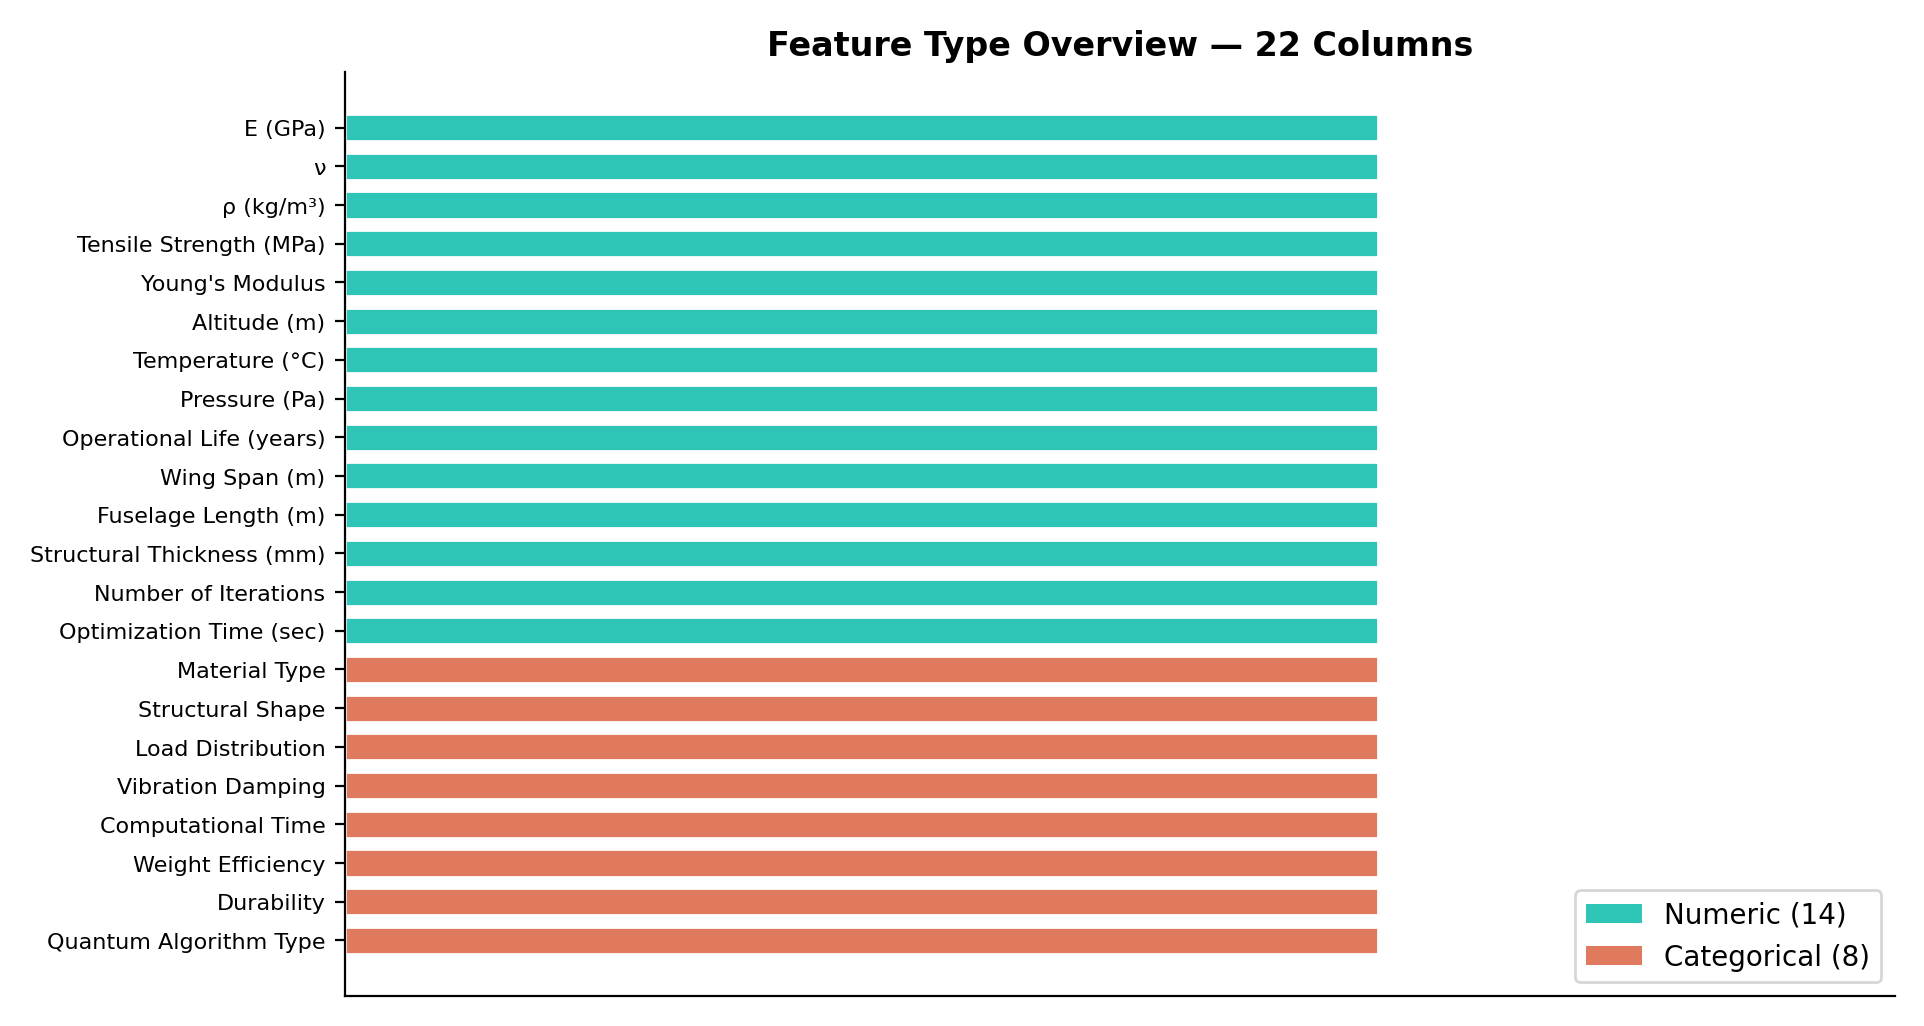
\includegraphics[width=0.85\textwidth]{ch2_feature_types}
\caption{Feature type overview. 14 numeric features (teal) and 8 categorical features (coral), including 4 target variables.}
\label{fig:feature_types}
\end{figure}

\section{Feature Catalog}

\begin{longtable}{p{4.5cm} c p{3.5cm} p{4.5cm}}
\toprule
\textbf{Feature} & \textbf{Type} & \textbf{Range / Values} & \textbf{Domain Interpretation} \\
\midrule
\endfirsthead
\toprule
\textbf{Feature} & \textbf{Type} & \textbf{Range / Values} & \textbf{Domain Interpretation} \\
\midrule
\endhead
Material Type & Categorical & Al / Ti / CF & Base structural material \\
E (GPa) & Numeric & 50.1 -- 199.8 & Elastic modulus (stiffness) \\
$\nu$ (Poisson) & Numeric & 0.30 -- 0.35 & Lateral strain ratio \\
$\rho$ (kg/m\textsuperscript{3}) & Numeric & 1{,}521 -- 4{,}496 & Material density \\
Tensile Strength (MPa) & Numeric & 261 -- 1{,}496 & Ultimate tensile strength \\
Young's Modulus & Numeric & 50 -- 99.6 & Secondary stiffness measure \\
Altitude (m) & Numeric & 5{,}086 -- 19{,}963 & Operating altitude \\
Temperature ($^{\circ}$C) & Numeric & $-60$ to $-40$ & Environmental temperature \\
Pressure (Pa) & Numeric & 100{,}172 -- 199{,}839 & Ambient pressure \\
Operational Life (years) & Integer & 20 -- 39 & Design service life \\
Wing Span (m) & Numeric & 20.0 -- 59.7 & Wing tip-to-tip span \\
Fuselage Length (m) & Numeric & 30.0 -- 70.0 & Fuselage length \\
Structural Thickness (mm) & Numeric & 5.0 -- 14.9 & Primary structural thickness \\
Structural Shape & Categorical & Rect / Cyl / Tapered & Cross-section geometry \\
Load Distribution & Categorical & uniform / point / distributed & Applied load pattern \\
Quantum Algorithm Type & Categorical & CQG / Shark Optimizer & Optimization algorithm \\
Number of Iterations & Integer & 523 -- 1{,}983 & Optimizer iterations \\
Optimization Time (sec) & Numeric & 51.5 -- 149.8 & Wall-clock convergence time \\
\midrule
\multicolumn{4}{l}{\textit{Target Variables (4 multi-class categorical):}} \\
\midrule
Vibration Damping & Target & High / Low / Moderate & Damping performance class \\
Computational Time & Target & Long / Medium / Short & Computation cost class \\
Weight Efficiency & Target & Excellent / Good / Poor & Mass optimization class \\
Durability & Target & High / Low / Medium & Structural longevity class \\
\bottomrule
\end{longtable}

\section{Data Quality}

\begin{figure}[H]
\centering
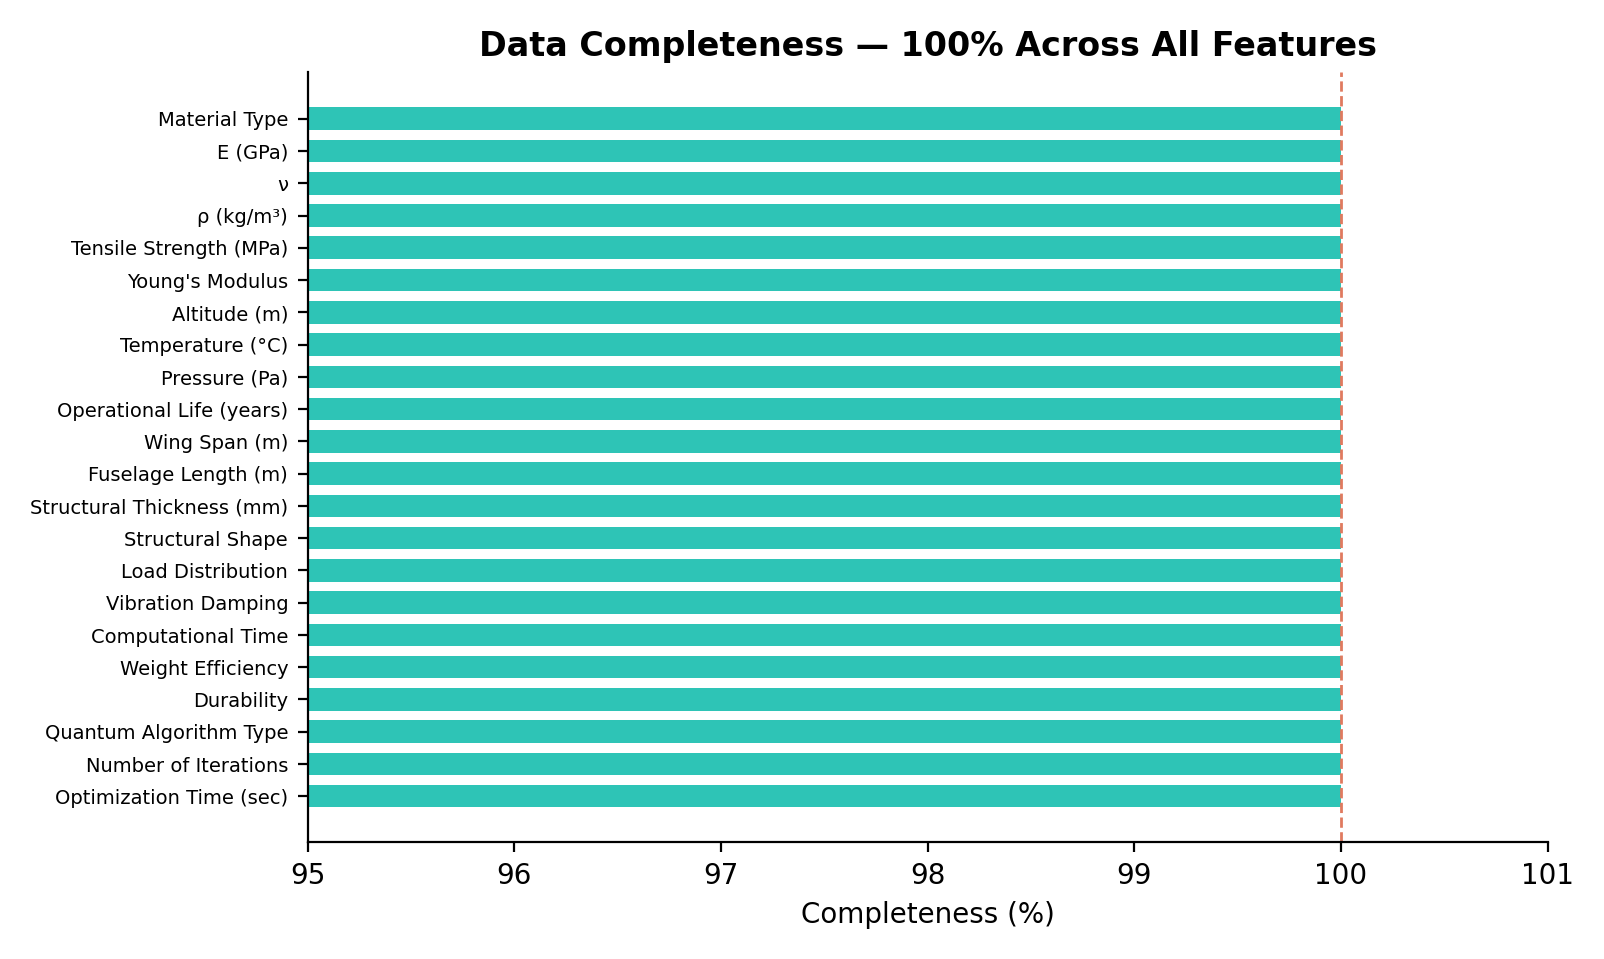
\includegraphics[width=0.75\textwidth]{ch2_completeness}
\caption{Data completeness: 100\% across all 22 features. Zero nulls, zero missing values.}
\label{fig:completeness}
\end{figure}

\begin{findingbox}
The dataset is impeccably clean: zero nulls, zero duplicates, consistent data types, and all values within physically plausible bounds. This cleanliness is consistent with simulation-generated data rather than field measurements.
\end{findingbox}


% ══════════════════════════════════════════════════════════════════════════════
\chapter{Univariate Analysis}
% ══════════════════════════════════════════════════════════════════════════════

This chapter examines every feature individually to characterize its marginal distribution, central tendency, dispersion, and shape.

\section{Numeric Features --- Overview}

\begin{figure}[H]
\centering
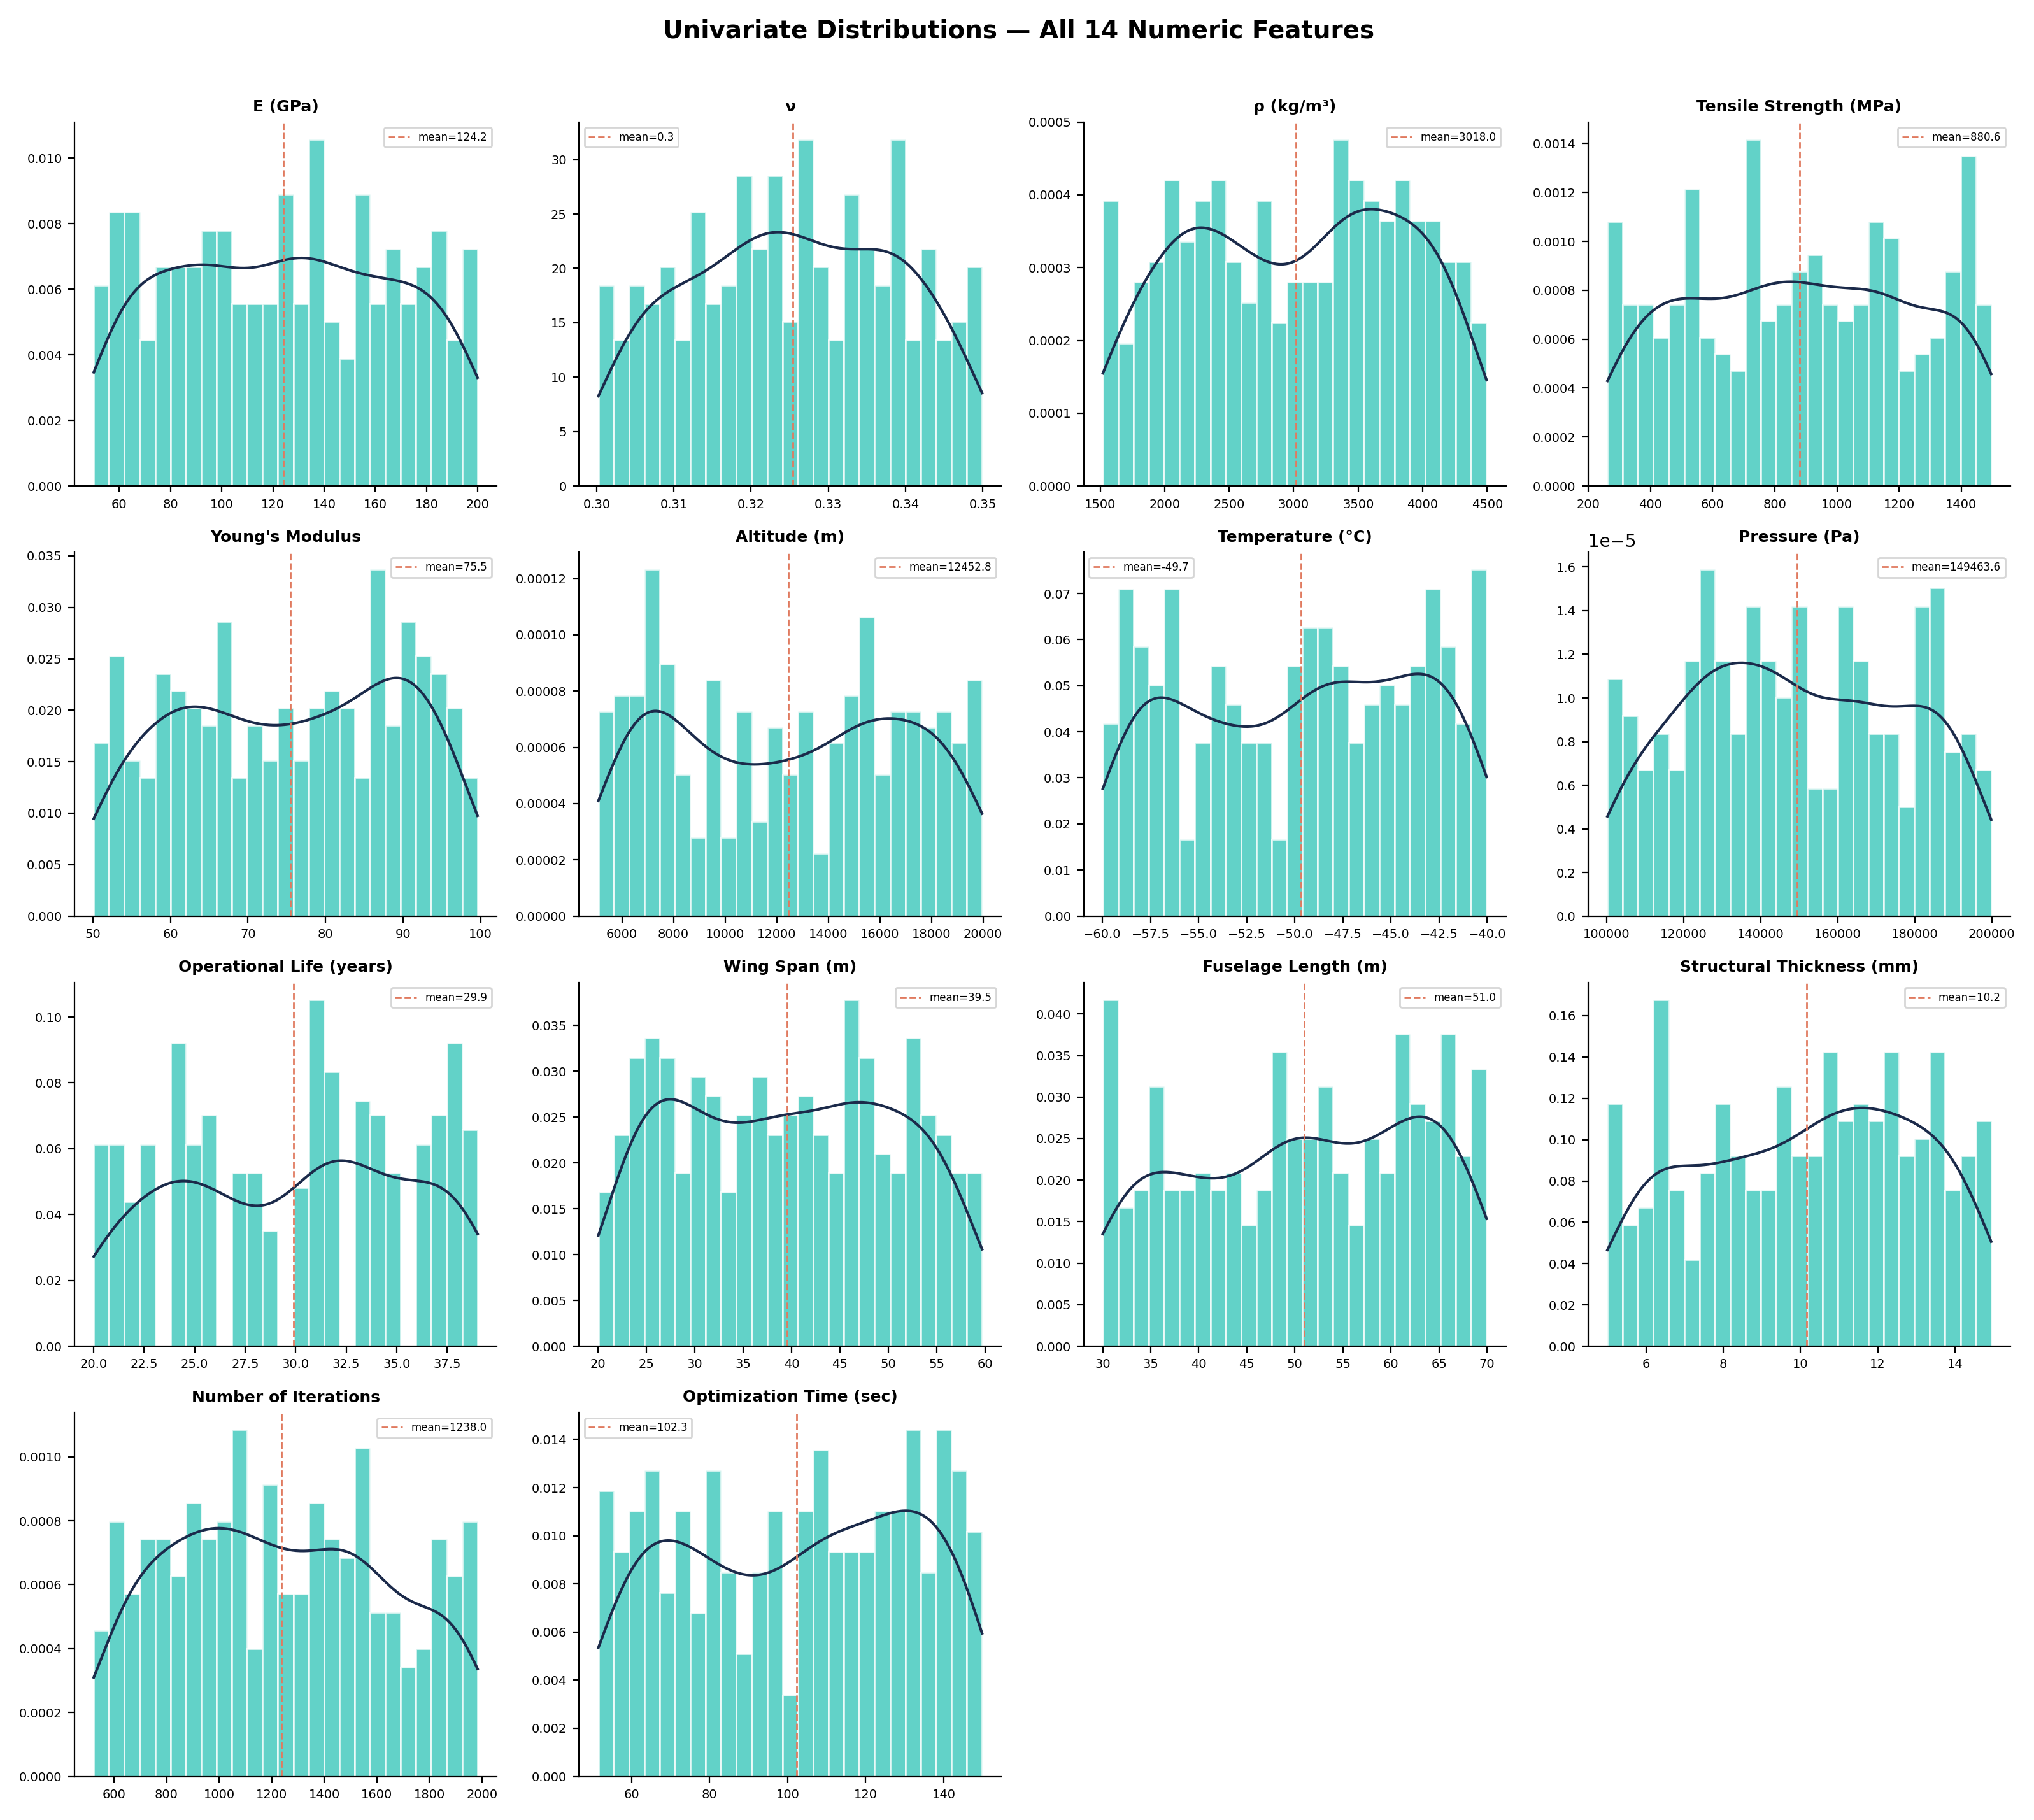
\includegraphics[width=\textwidth]{ch3_univariate_numeric_grid}
\caption{Distribution of all 14 numeric features. Histograms with KDE overlay and mean line (red dashed). All distributions are approximately uniform with platykurtic shape (negative kurtosis).}
\label{fig:univariate_grid}
\end{figure}

\subsection{Summary Statistics}

\begin{table}[H]
\centering
\caption{Descriptive statistics for all 14 numeric features. All features fail the Shapiro--Wilk normality test at $\alpha = 0.05$.}
\label{tab:univariate}
\footnotesize
\begin{tabular}{lrrrrrrr}
\toprule
\textbf{Feature} & \textbf{Mean} & \textbf{Std} & \textbf{Min} & \textbf{Median} & \textbf{Max} & \textbf{Skew} & \textbf{Kurt.} \\
\midrule
E (GPa)               & 124.21 & 43.39 &  50.10 & 125.09 & 199.84 &  0.033 & $-$1.17 \\
$\nu$                  &   0.33 &  0.01 &   0.30 &   0.33 &   0.35 & $-$0.042 & $-$1.05 \\
$\rho$ (kg/m$^3$)     & 3018.0 & 843.3 & 1520.9 & 3071.5 & 4495.8 & $-$0.063 & $-$1.21 \\
Tensile (MPa)          & 880.6  & 363.3 &  261.2 &  883.3 & 1496.1 & $-$0.002 & $-$1.18 \\
Young's Mod.           &  75.46 & 14.28 &  50.11 &  76.00 &  99.61 & $-$0.087 & $-$1.24 \\
Altitude (m)           & 12453  &  4545 &   5086 &  12587 &  19963 & $-$0.009 & $-$1.36 \\
Temperature ($^\circ$C) & $-$49.7 &   6.0 & $-$60.0 & $-$49.0 & $-$40.0 & $-$0.093 & $-$1.28 \\
Pressure (Pa)          & 149464 & 27866 & 100172 & 147943 & 199839 &  0.041 & $-$1.13 \\
Op.\ Life (yr)         &  29.88 &  5.79 &  20.00 &  31.00 &  39.00 & $-$0.084 & $-$1.22 \\
Wing Span (m)          &  39.52 & 11.22 &  20.02 &  39.37 &  59.70 &  0.020 & $-$1.22 \\
Fuselage (m)           &  50.99 & 12.03 &  30.01 &  51.65 &  69.96 & $-$0.159 & $-$1.21 \\
Thickness (mm)         &  10.17 &  2.84 &   5.00 &  10.44 &  14.94 & $-$0.141 & $-$1.13 \\
Iterations             &  1238  &   411 &    523 &   1218 &   1983 &  0.120 & $-$1.10 \\
Opt.\ Time (sec)       & 102.26 & 29.60 &  51.45 & 105.82 & 149.83 & $-$0.100 & $-$1.29 \\
\bottomrule
\end{tabular}
\end{table}

\begin{findingbox}
Every numeric feature exhibits a kurtosis between $-1.10$ and $-1.36$, strongly indicative of uniform or near-uniform distributions bounded by design constraints. Skewness values are near-zero ($|$skew$| < 0.16$), confirming symmetric distributions. The coefficient of variation (CV) ranges from 4.3\% ($\nu$) to 35.0\% (E), reflecting the varying breadth of each feature's design space.
\end{findingbox}

\section{Detailed Feature Profiles}

\subsection{Elastic Modulus --- E (GPa)}

\begin{figure}[H]
\centering
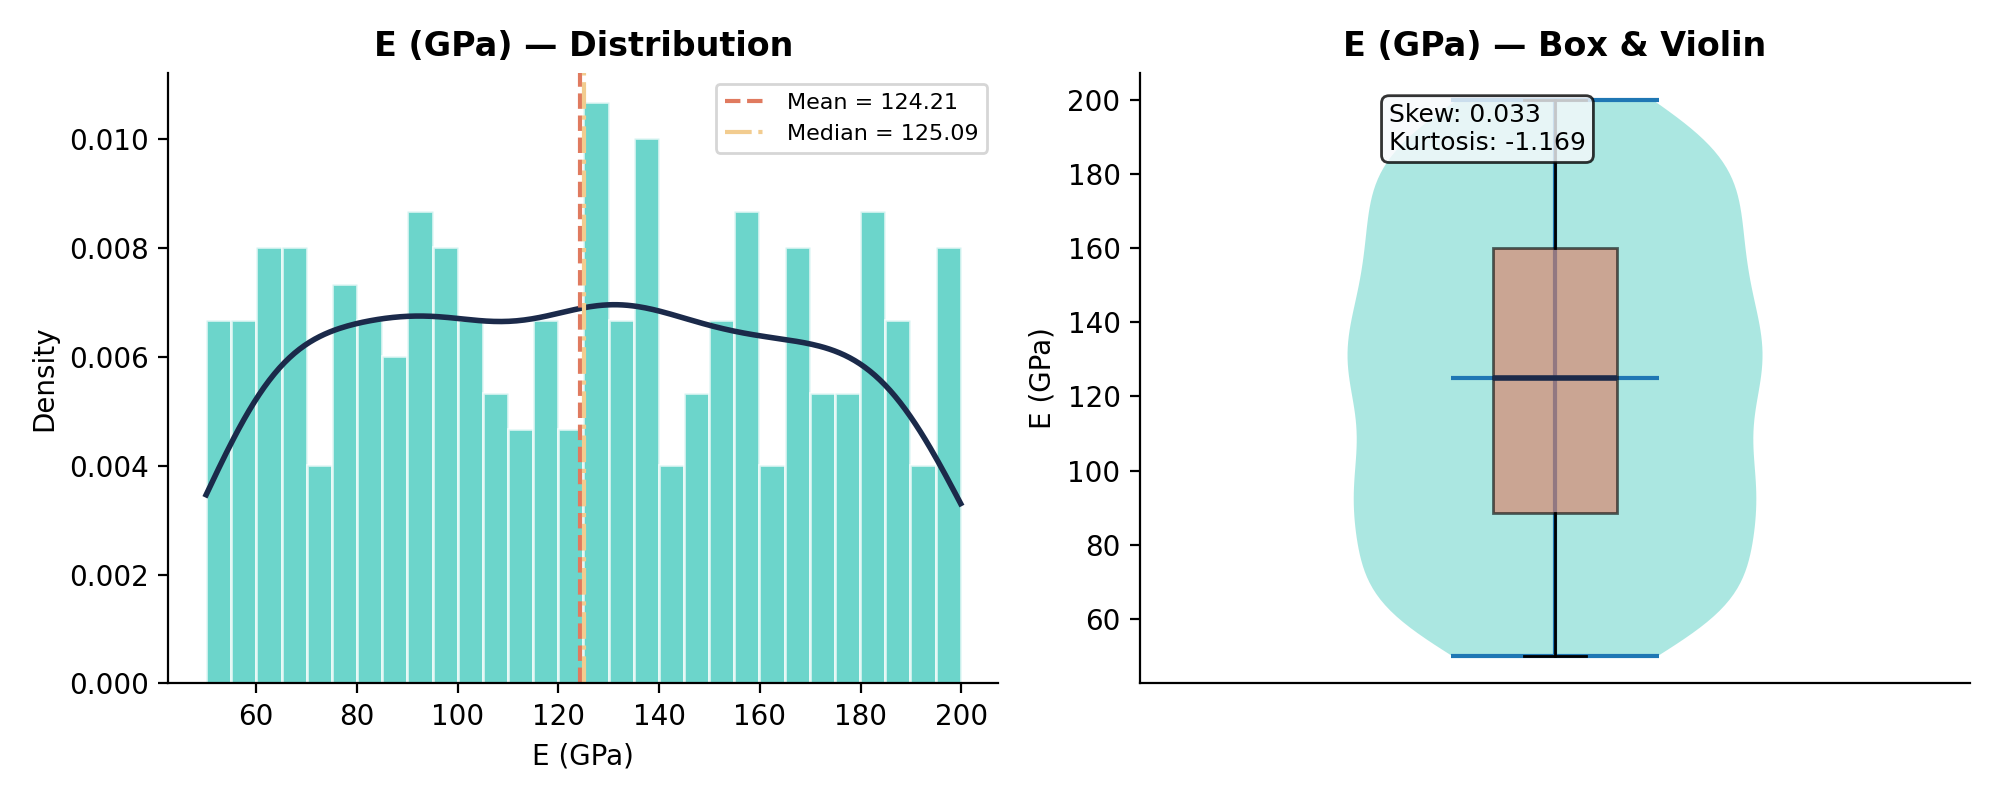
\includegraphics[width=0.95\textwidth]{ch3_univar_E_GPa}
\caption{E (GPa) distribution and box-violin plot. The tri-modal structure corresponding to Aluminum ($\sim$50--100), Titanium ($\sim$100--150), and Carbon Fiber ($\sim$150--200) is visible as a broad plateau.}
\label{fig:e_gpa}
\end{figure}

The elastic modulus is the most physically informative feature in the dataset. Its range of 50.1--199.8~GPa spans the full spectrum of aerospace-grade materials:
\begin{itemize}[nosep]
\item \textbf{Aluminum alloys:} $E \approx 50$--$100$~GPa (2xxx/7xxx series)
\item \textbf{Titanium alloys:} $E \approx 100$--$150$~GPa (Ti-6Al-4V range)
\item \textbf{Carbon Fiber composites:} $E \approx 150$--$200$~GPa (high-modulus CFRP)
\end{itemize}

\subsection{Tensile Strength (MPa)}

\begin{figure}[H]
\centering
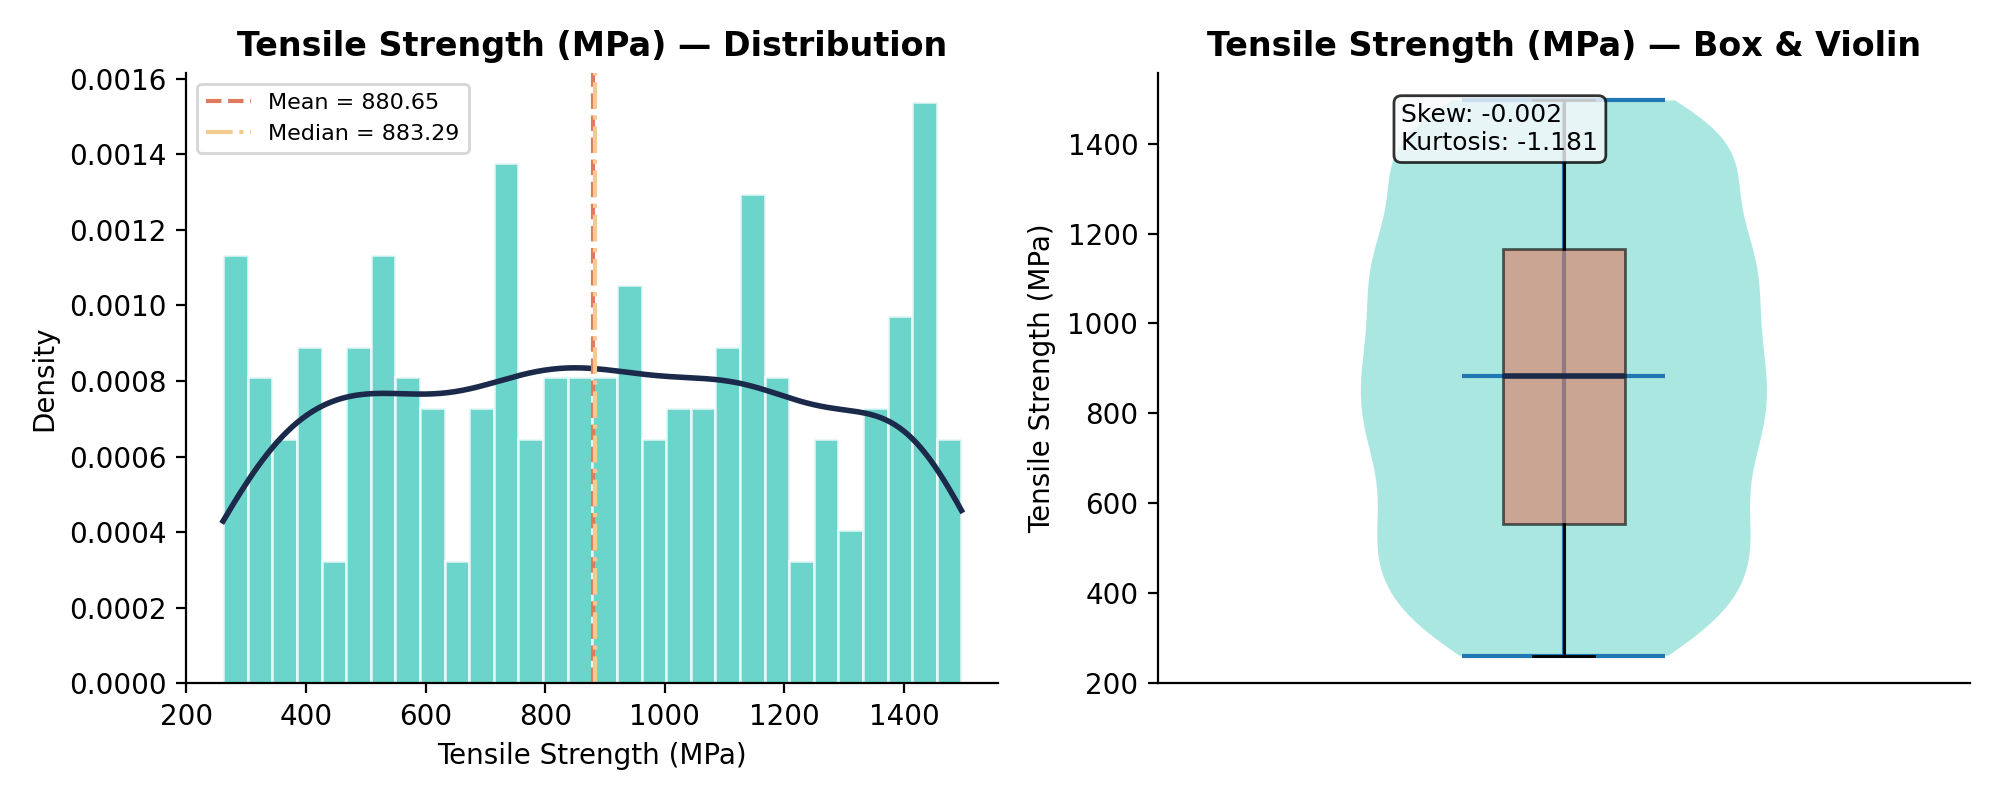
\includegraphics[width=0.95\textwidth]{ch3_univar_Tensile_Strength_MPa}
\caption{Tensile Strength distribution. Approximately uniform across the full 261--1{,}496~MPa range.}
\label{fig:tensile}
\end{figure}

\subsection{Altitude and Temperature}

\begin{figure}[H]
\centering
\begin{subfigure}{0.48\textwidth}
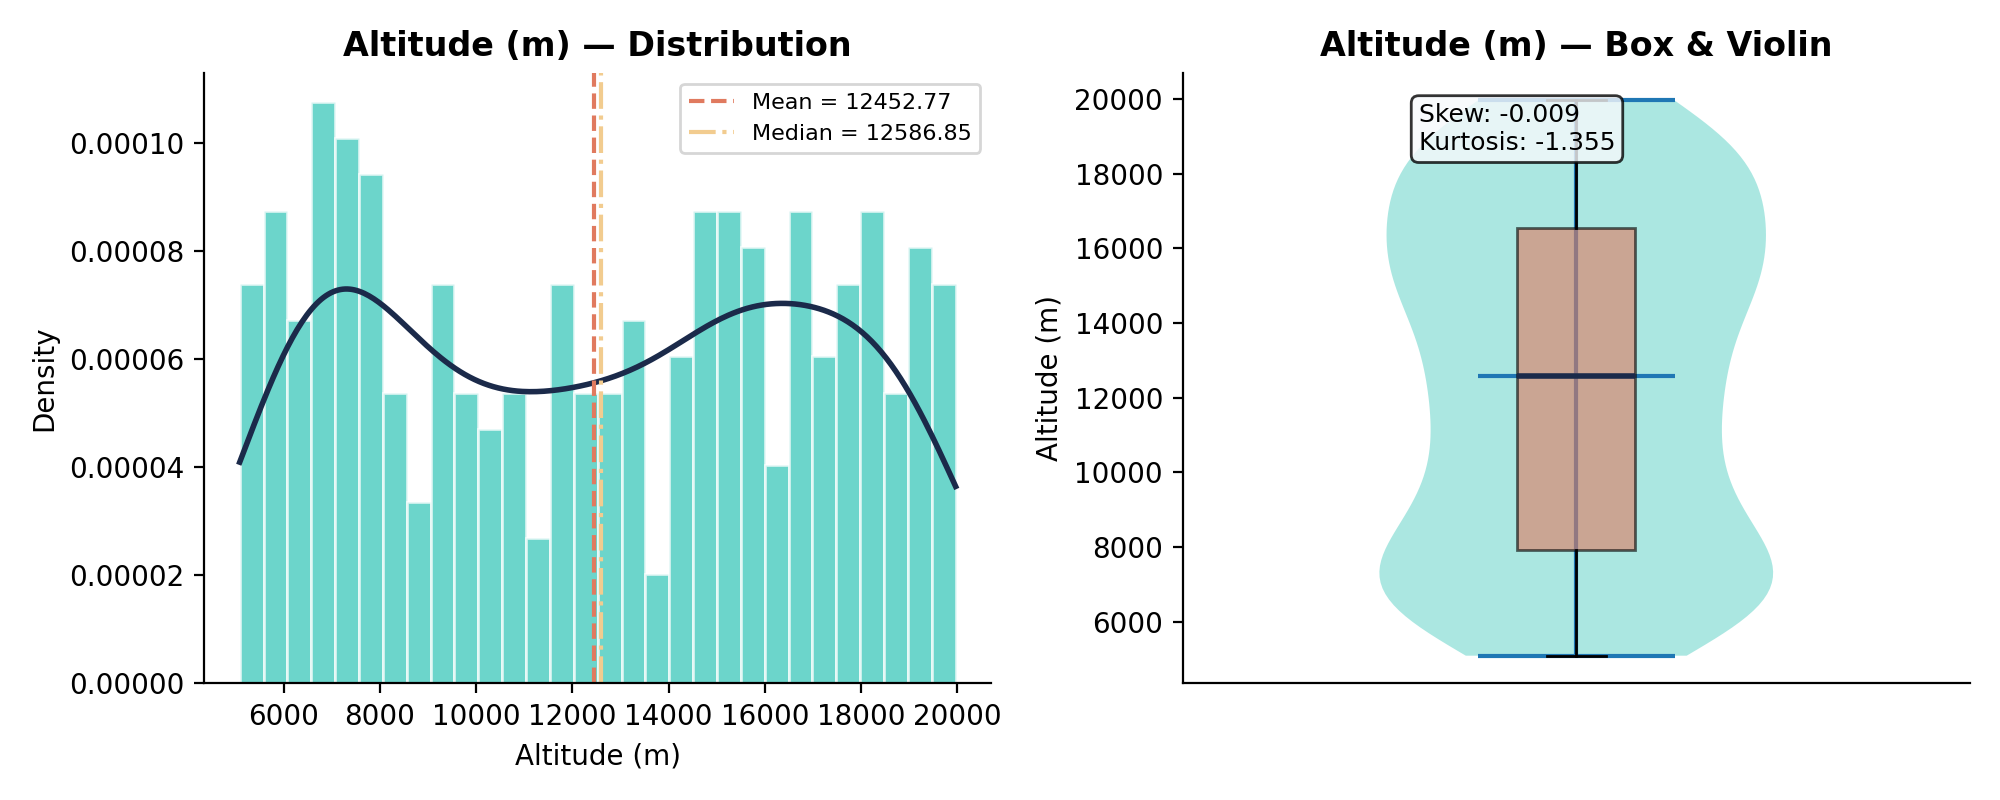
\includegraphics[width=\textwidth]{ch3_univar_Altitude_m}
\caption{Altitude (m)}
\end{subfigure}
\hfill
\begin{subfigure}{0.48\textwidth}
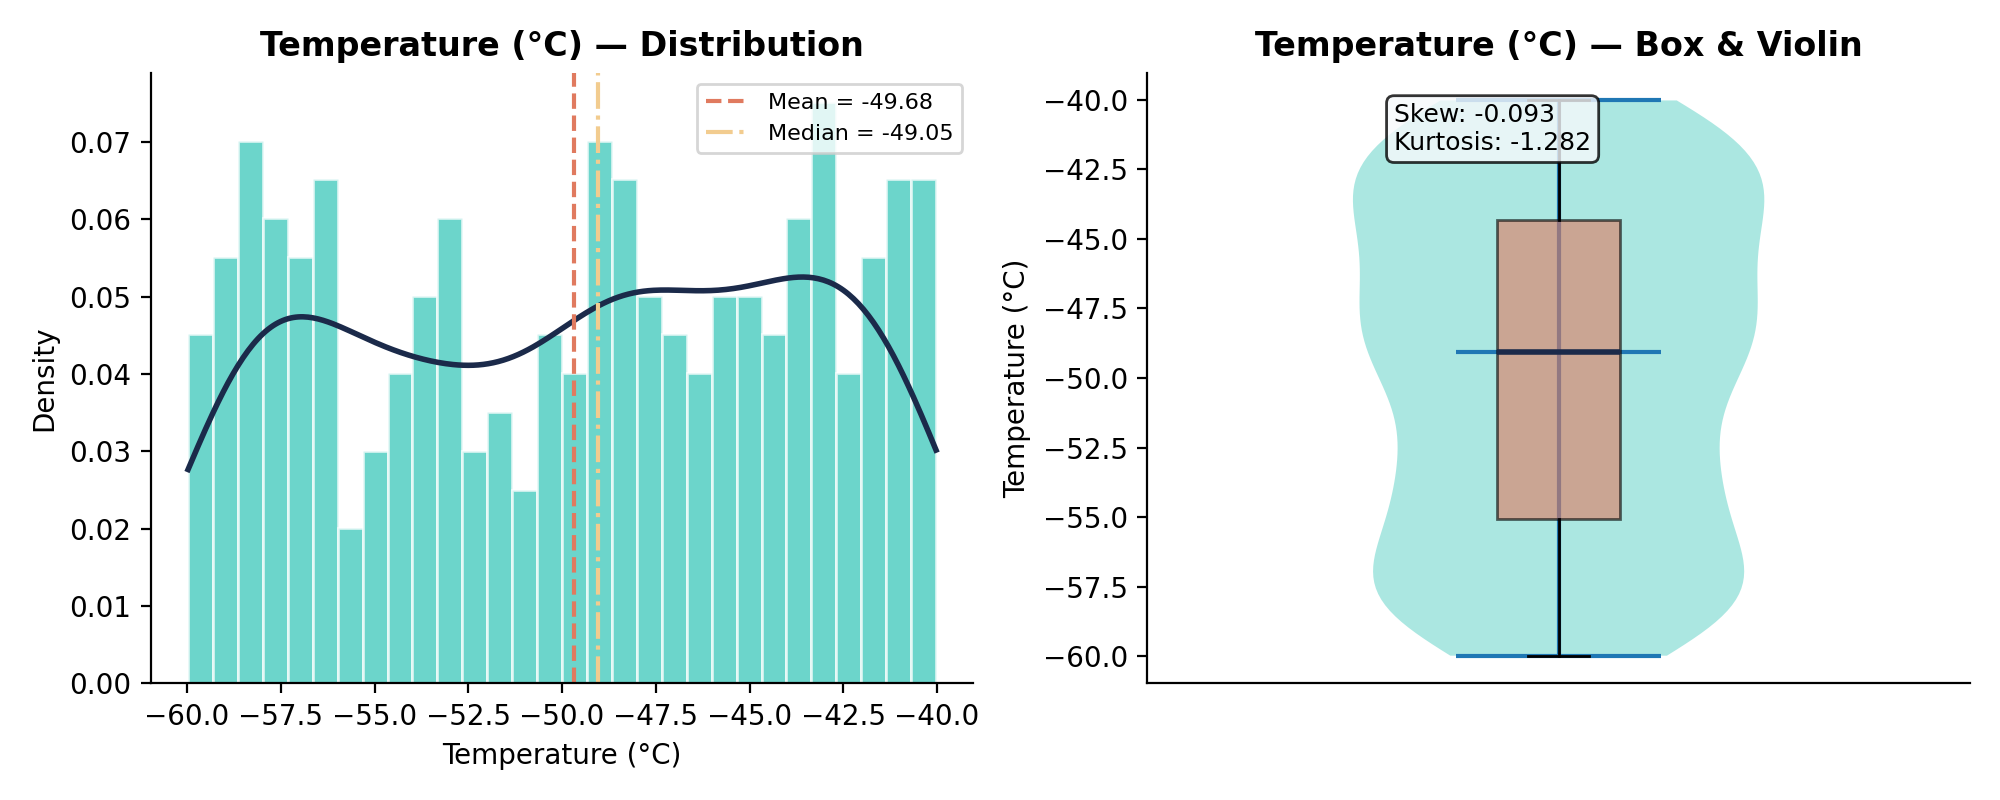
\includegraphics[width=\textwidth]{ch3_univar_Temperature_degC}
\caption{Temperature ($^{\circ}$C)}
\end{subfigure}
\caption{Flight environment features. Altitude spans 5{,}086--19{,}963~m (commercial to near-stratospheric). Temperature is constrained to $-60$ to $-40\,^{\circ}$C.}
\label{fig:flight_env}
\end{figure}

\subsection{Pressure and Young's Modulus}

\begin{figure}[H]
\centering
\begin{subfigure}{0.48\textwidth}
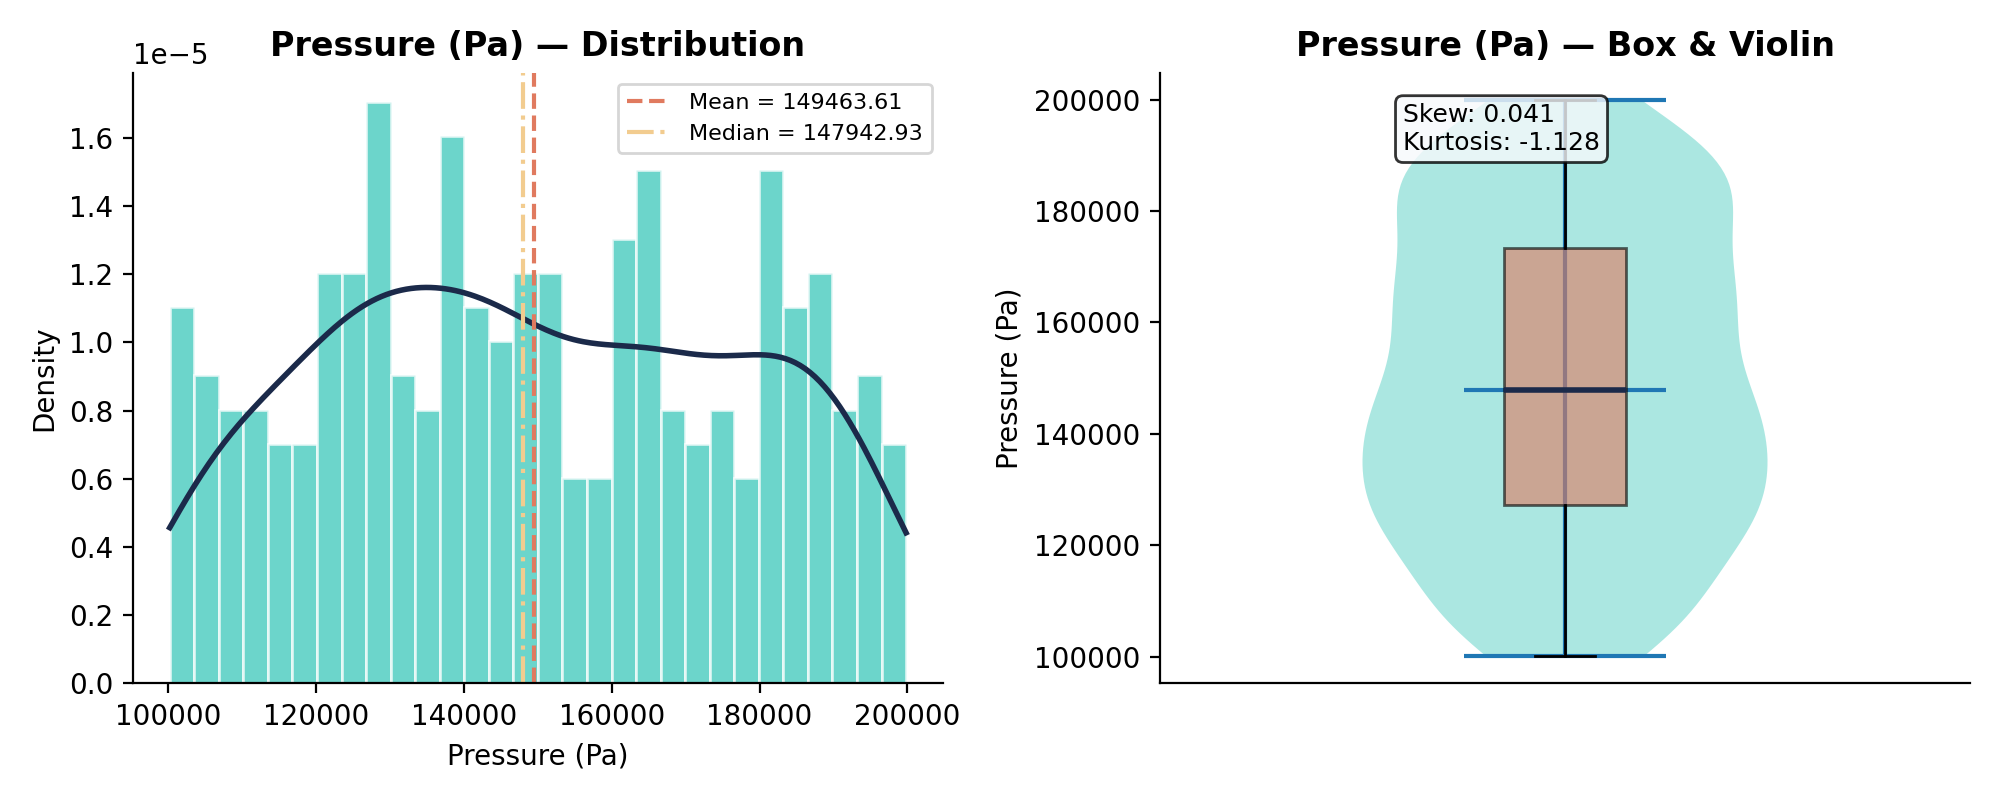
\includegraphics[width=\textwidth]{ch3_univar_Pressure_Pa}
\caption{Pressure (Pa)}
\end{subfigure}
\hfill
\begin{subfigure}{0.48\textwidth}
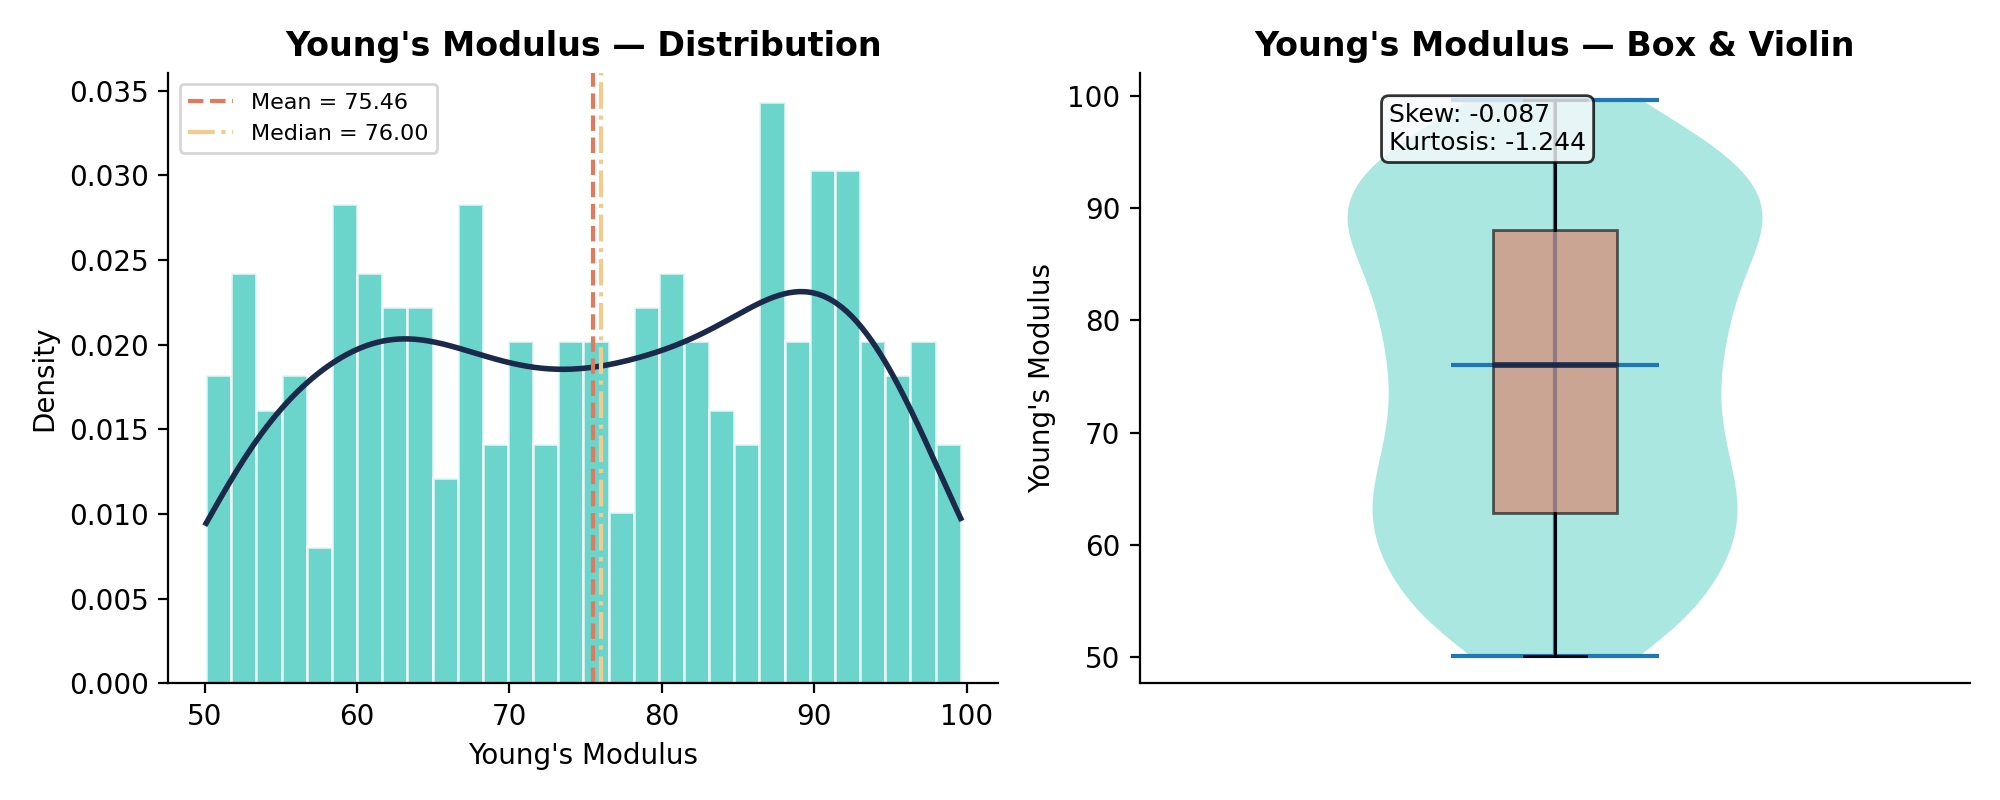
\includegraphics[width=\textwidth]{ch3_univar_Youngs_Modulus}
\caption{Young's Modulus}
\end{subfigure}
\caption{Pressure spans 100{,}172--199{,}839~Pa (near sea-level range, anomalous at high altitude). Young's Modulus is a secondary stiffness measure confined to 50--99.6.}
\label{fig:pressure_ym}
\end{figure}

\subsection{Wing Span}

\begin{figure}[H]
\centering
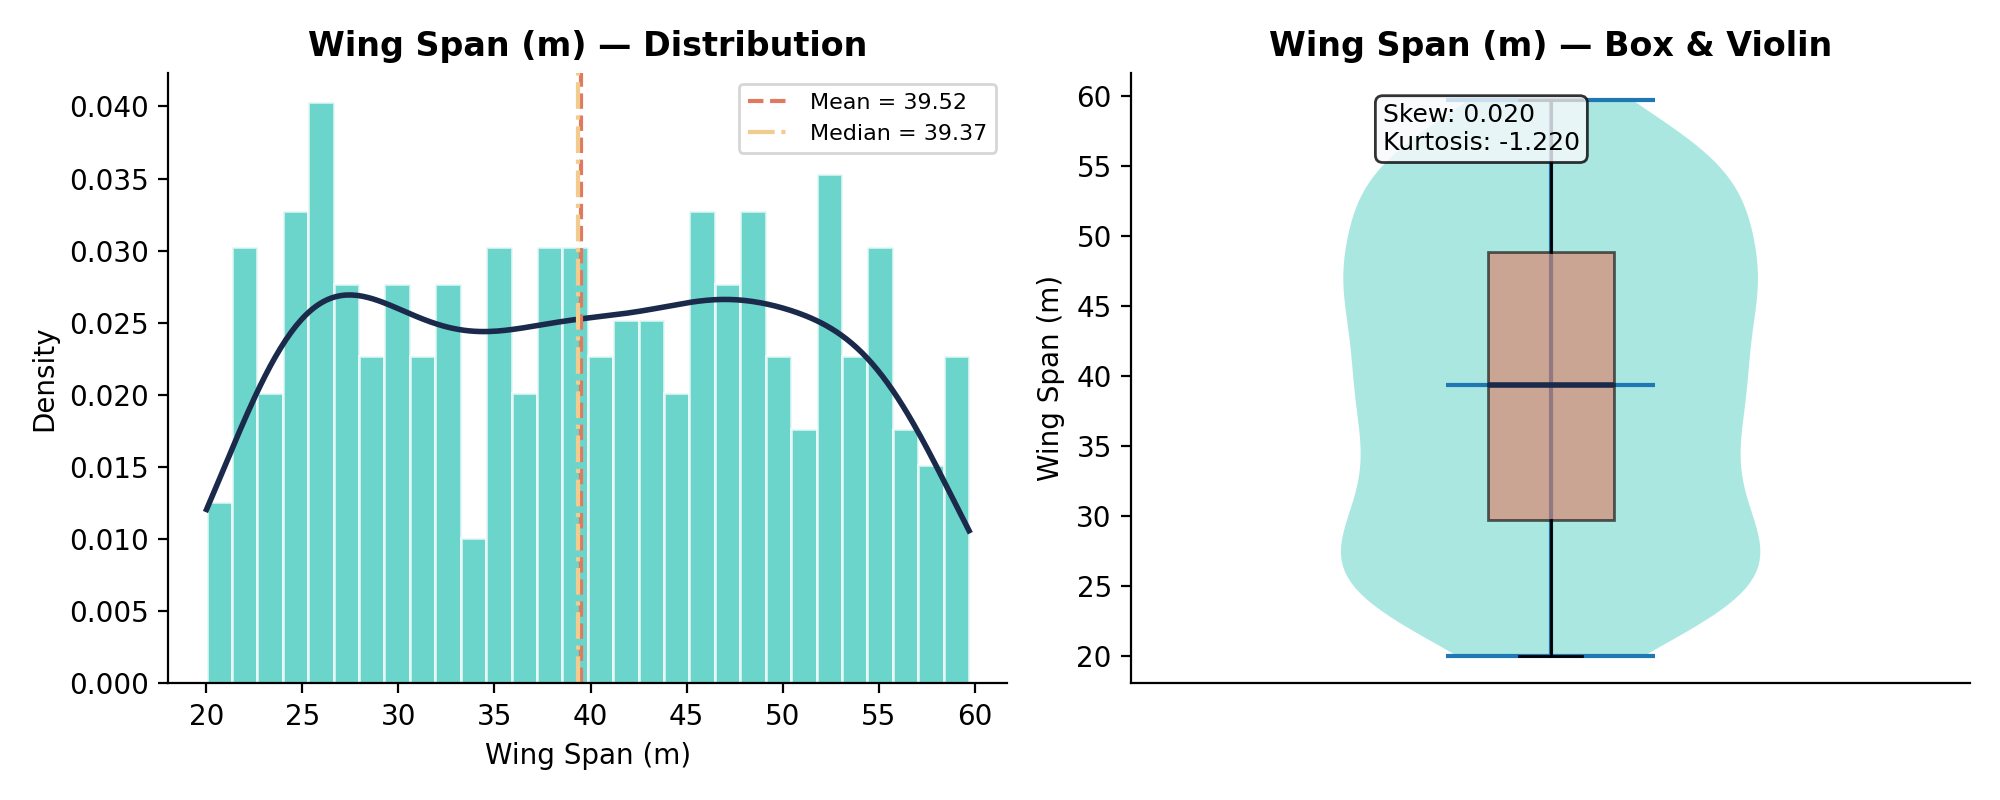
\includegraphics[width=0.95\textwidth]{ch3_univar_Wing_Span_m}
\caption{Wing Span distribution. Range of 20--59.7~m covers regional jets through wide-body aircraft.}
\label{fig:wingspan}
\end{figure}

\section{Categorical Features}

\begin{figure}[H]
\centering
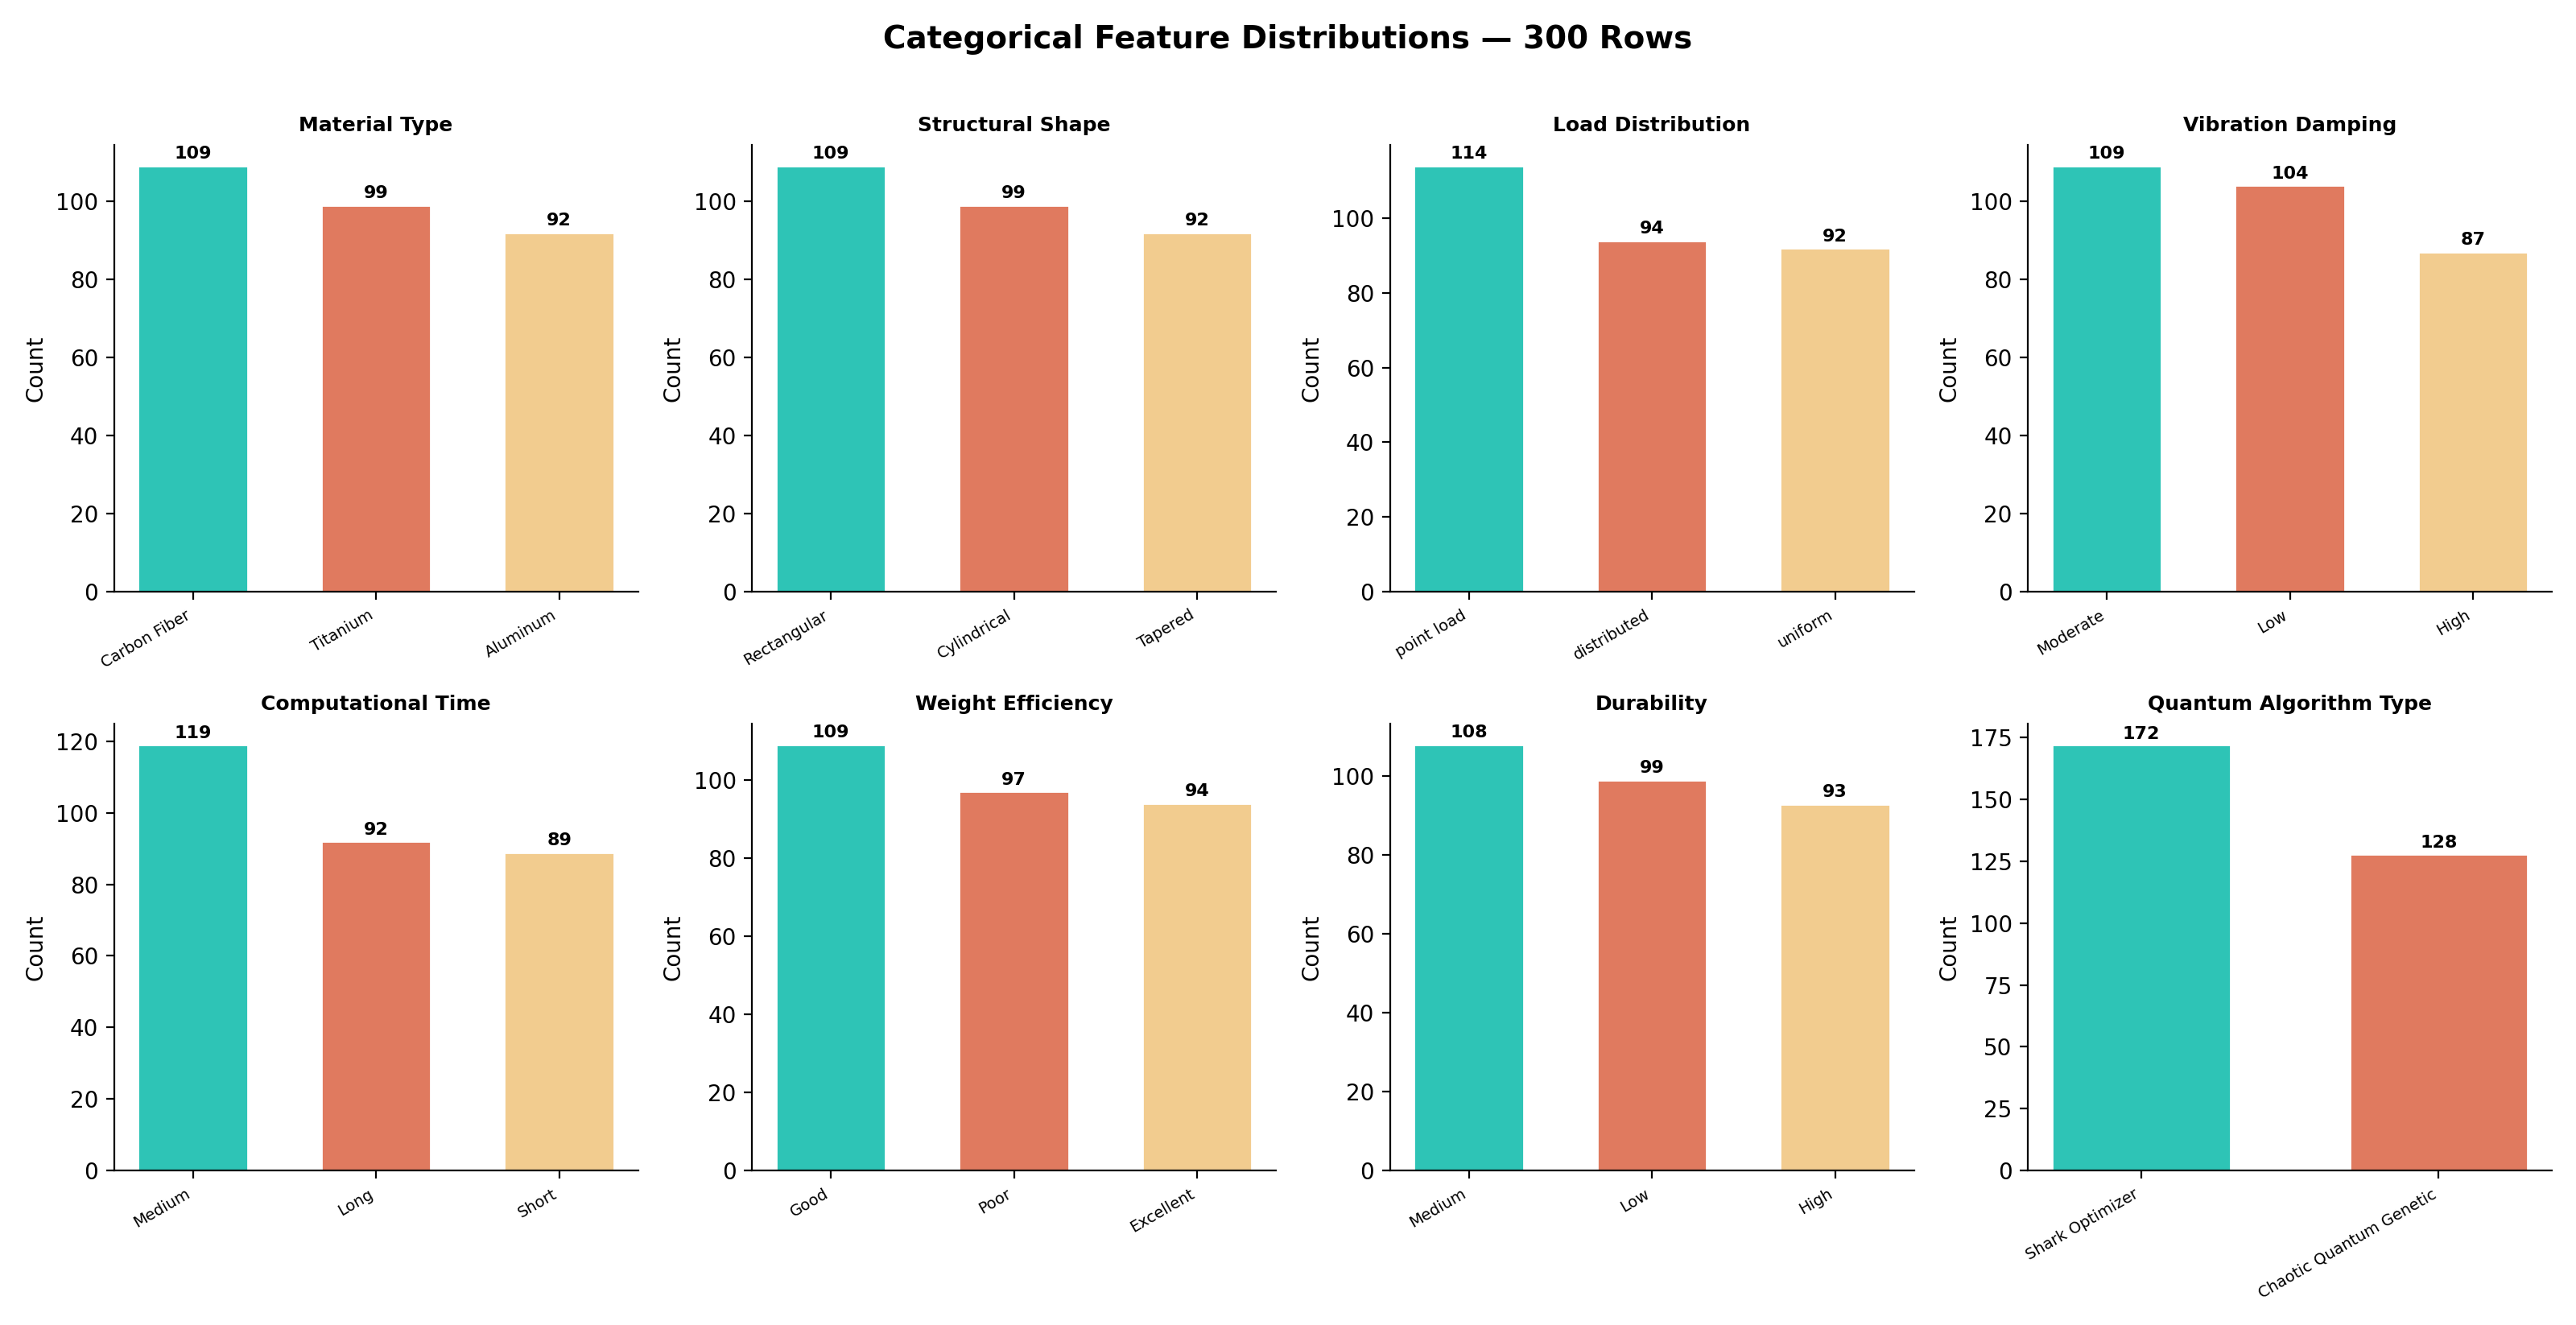
\includegraphics[width=\textwidth]{ch3_categorical_grid}
\caption{Distribution of all 8 categorical features. Most features have 3 levels with approximate balance. Quantum Algorithm Type is binary (Shark Optimizer: 172, Chaotic Quantum Genetic: 128).}
\label{fig:categorical}
\end{figure}

\begin{table}[H]
\centering
\caption{Categorical feature summary. Balance ratio = min\_count / max\_count; closer to 1.0 indicates better balance.}
\label{tab:categorical}
\footnotesize
\begin{tabular}{lccc}
\toprule
\textbf{Feature} & \textbf{Levels} & \textbf{Mode (count)} & \textbf{Balance Ratio} \\
\midrule
Material Type          & 3 & Carbon Fiber (109) & 0.844 \\
Structural Shape       & 3 & Rectangular (109)  & 0.844 \\
Load Distribution      & 3 & Point Load (114)   & 0.807 \\
Vibration Damping      & 3 & Moderate (109)     & 0.798 \\
Computational Time     & 3 & Medium (119)       & 0.748 \\
Weight Efficiency      & 3 & Good (109)         & 0.862 \\
Durability             & 3 & Medium (108)       & 0.861 \\
Quantum Algorithm Type & 2 & Shark Opt.\ (172)  & 0.744 \\
\bottomrule
\end{tabular}
\end{table}


% ══════════════════════════════════════════════════════════════════════════════
\chapter{Bivariate \& Multivariate Analysis}
% ══════════════════════════════════════════════════════════════════════════════

\section{Correlation Analysis}

\begin{figure}[H]
\centering
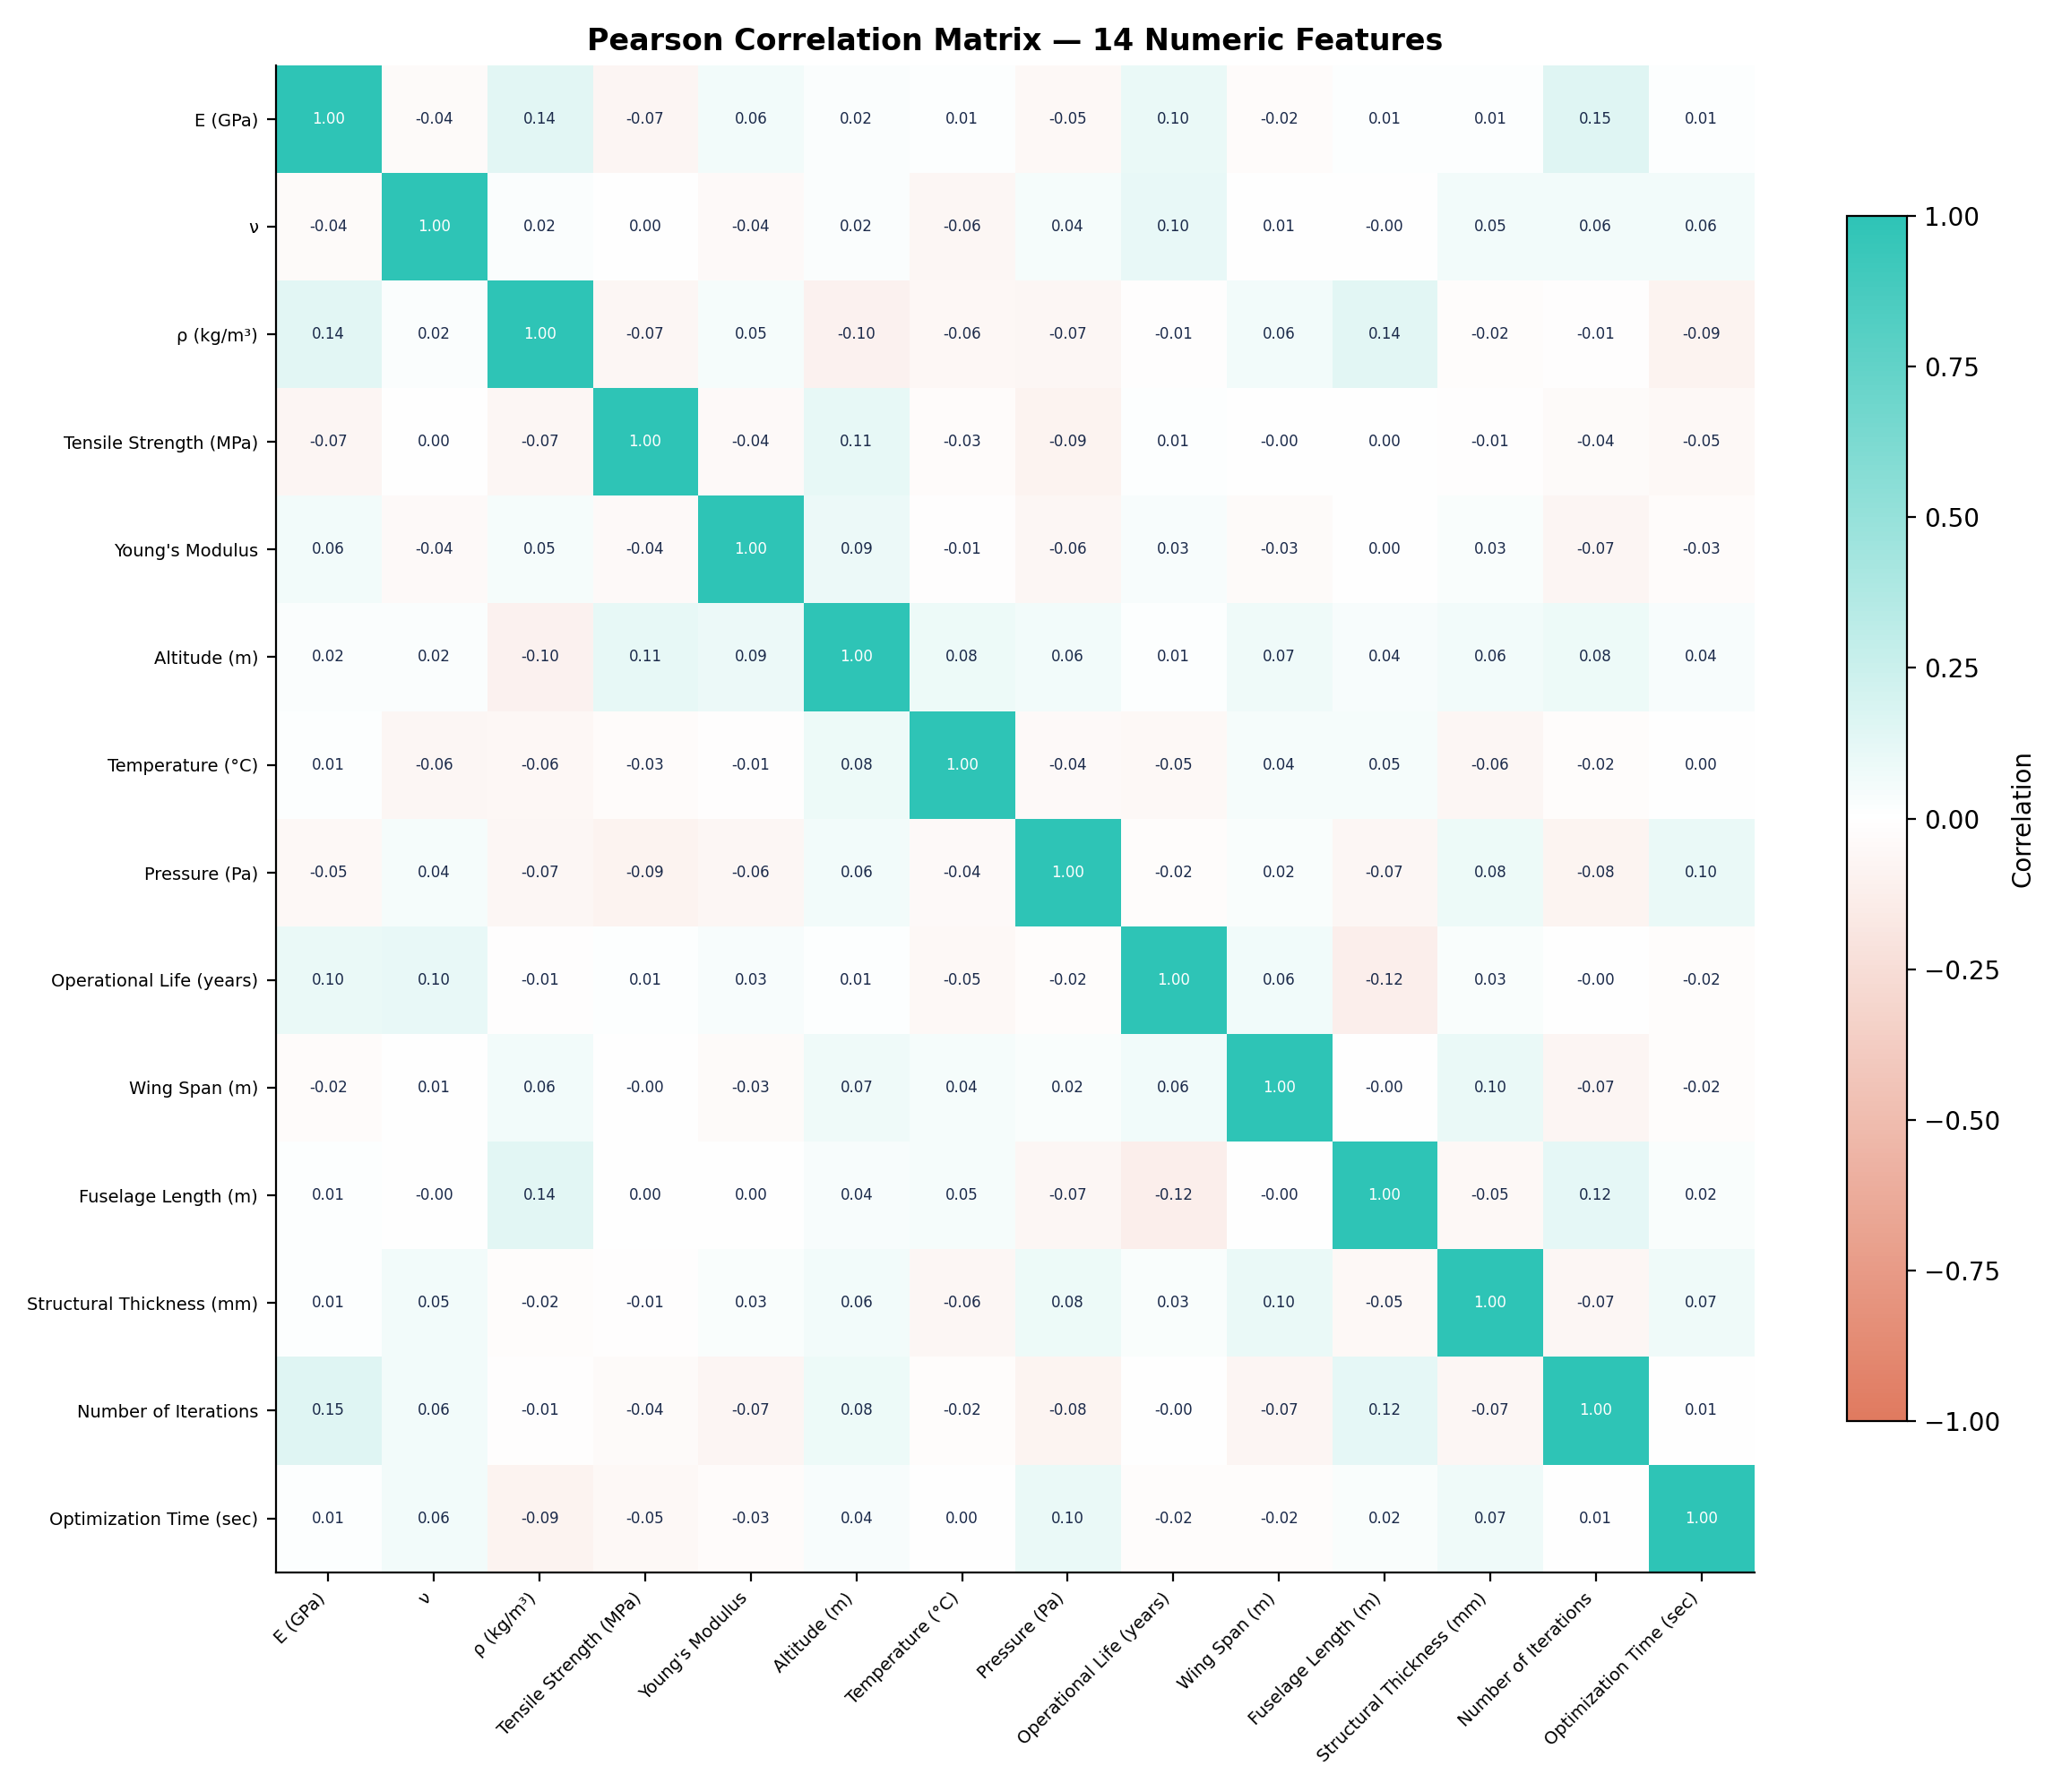
\includegraphics[width=0.9\textwidth]{ch4_correlation_pearson}
\caption{Pearson correlation matrix. All pairwise correlations are weak ($|r| < 0.10$), indicating near-complete linear independence among numeric features.}
\label{fig:corr_pearson}
\end{figure}

\begin{figure}[H]
\centering
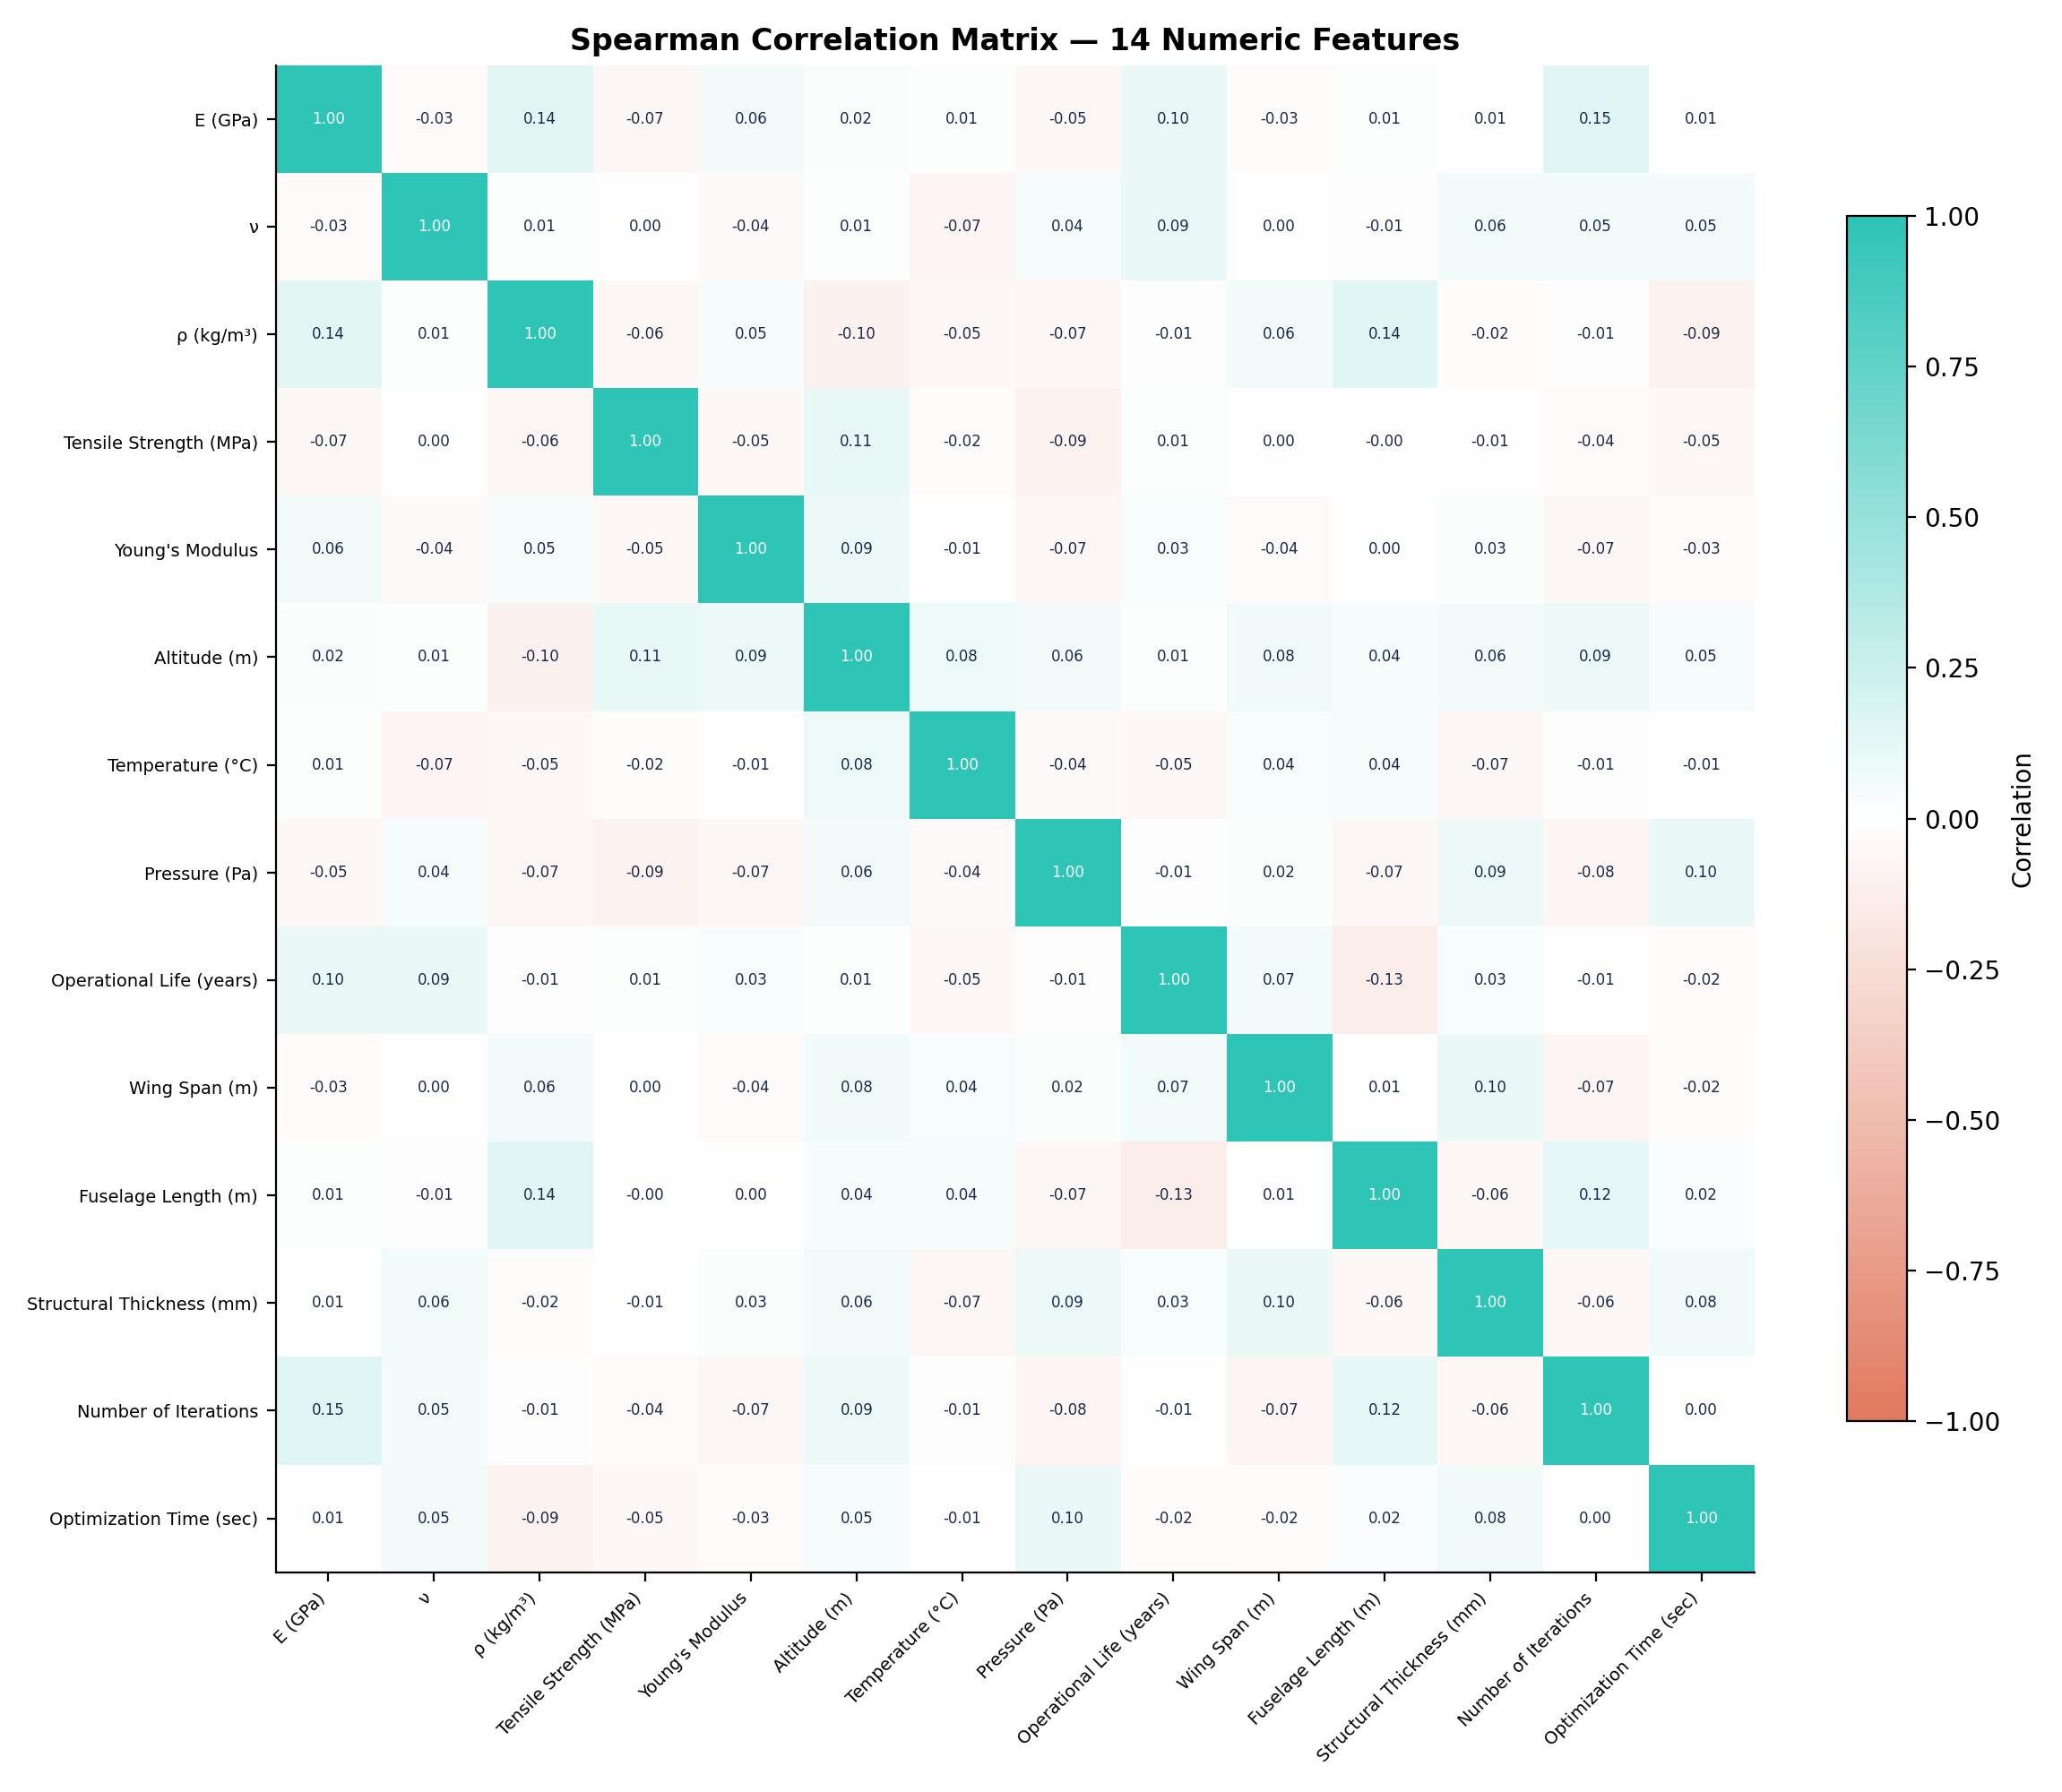
\includegraphics[width=0.9\textwidth]{ch4_correlation_spearman}
\caption{Spearman rank correlation matrix. Consistent with Pearson results, confirming the absence of both linear and monotonic relationships.}
\label{fig:corr_spearman}
\end{figure}

\begin{findingbox}
The near-zero correlation structure is the most distinctive statistical property of this dataset. No pair of numeric features exceeds $|r| = 0.10$. This orthogonality implies:
\begin{itemize}[nosep]
\item Features were sampled independently in the simulation design
\item Correlation preservation is a trivially satisfied benchmark for synthetic generators
\item The real challenge for generators lies in preserving marginal distributions and categorical structure, not joint dependencies
\end{itemize}
\end{findingbox}

\section{Key Bivariate Relationships}

\begin{figure}[H]
\centering
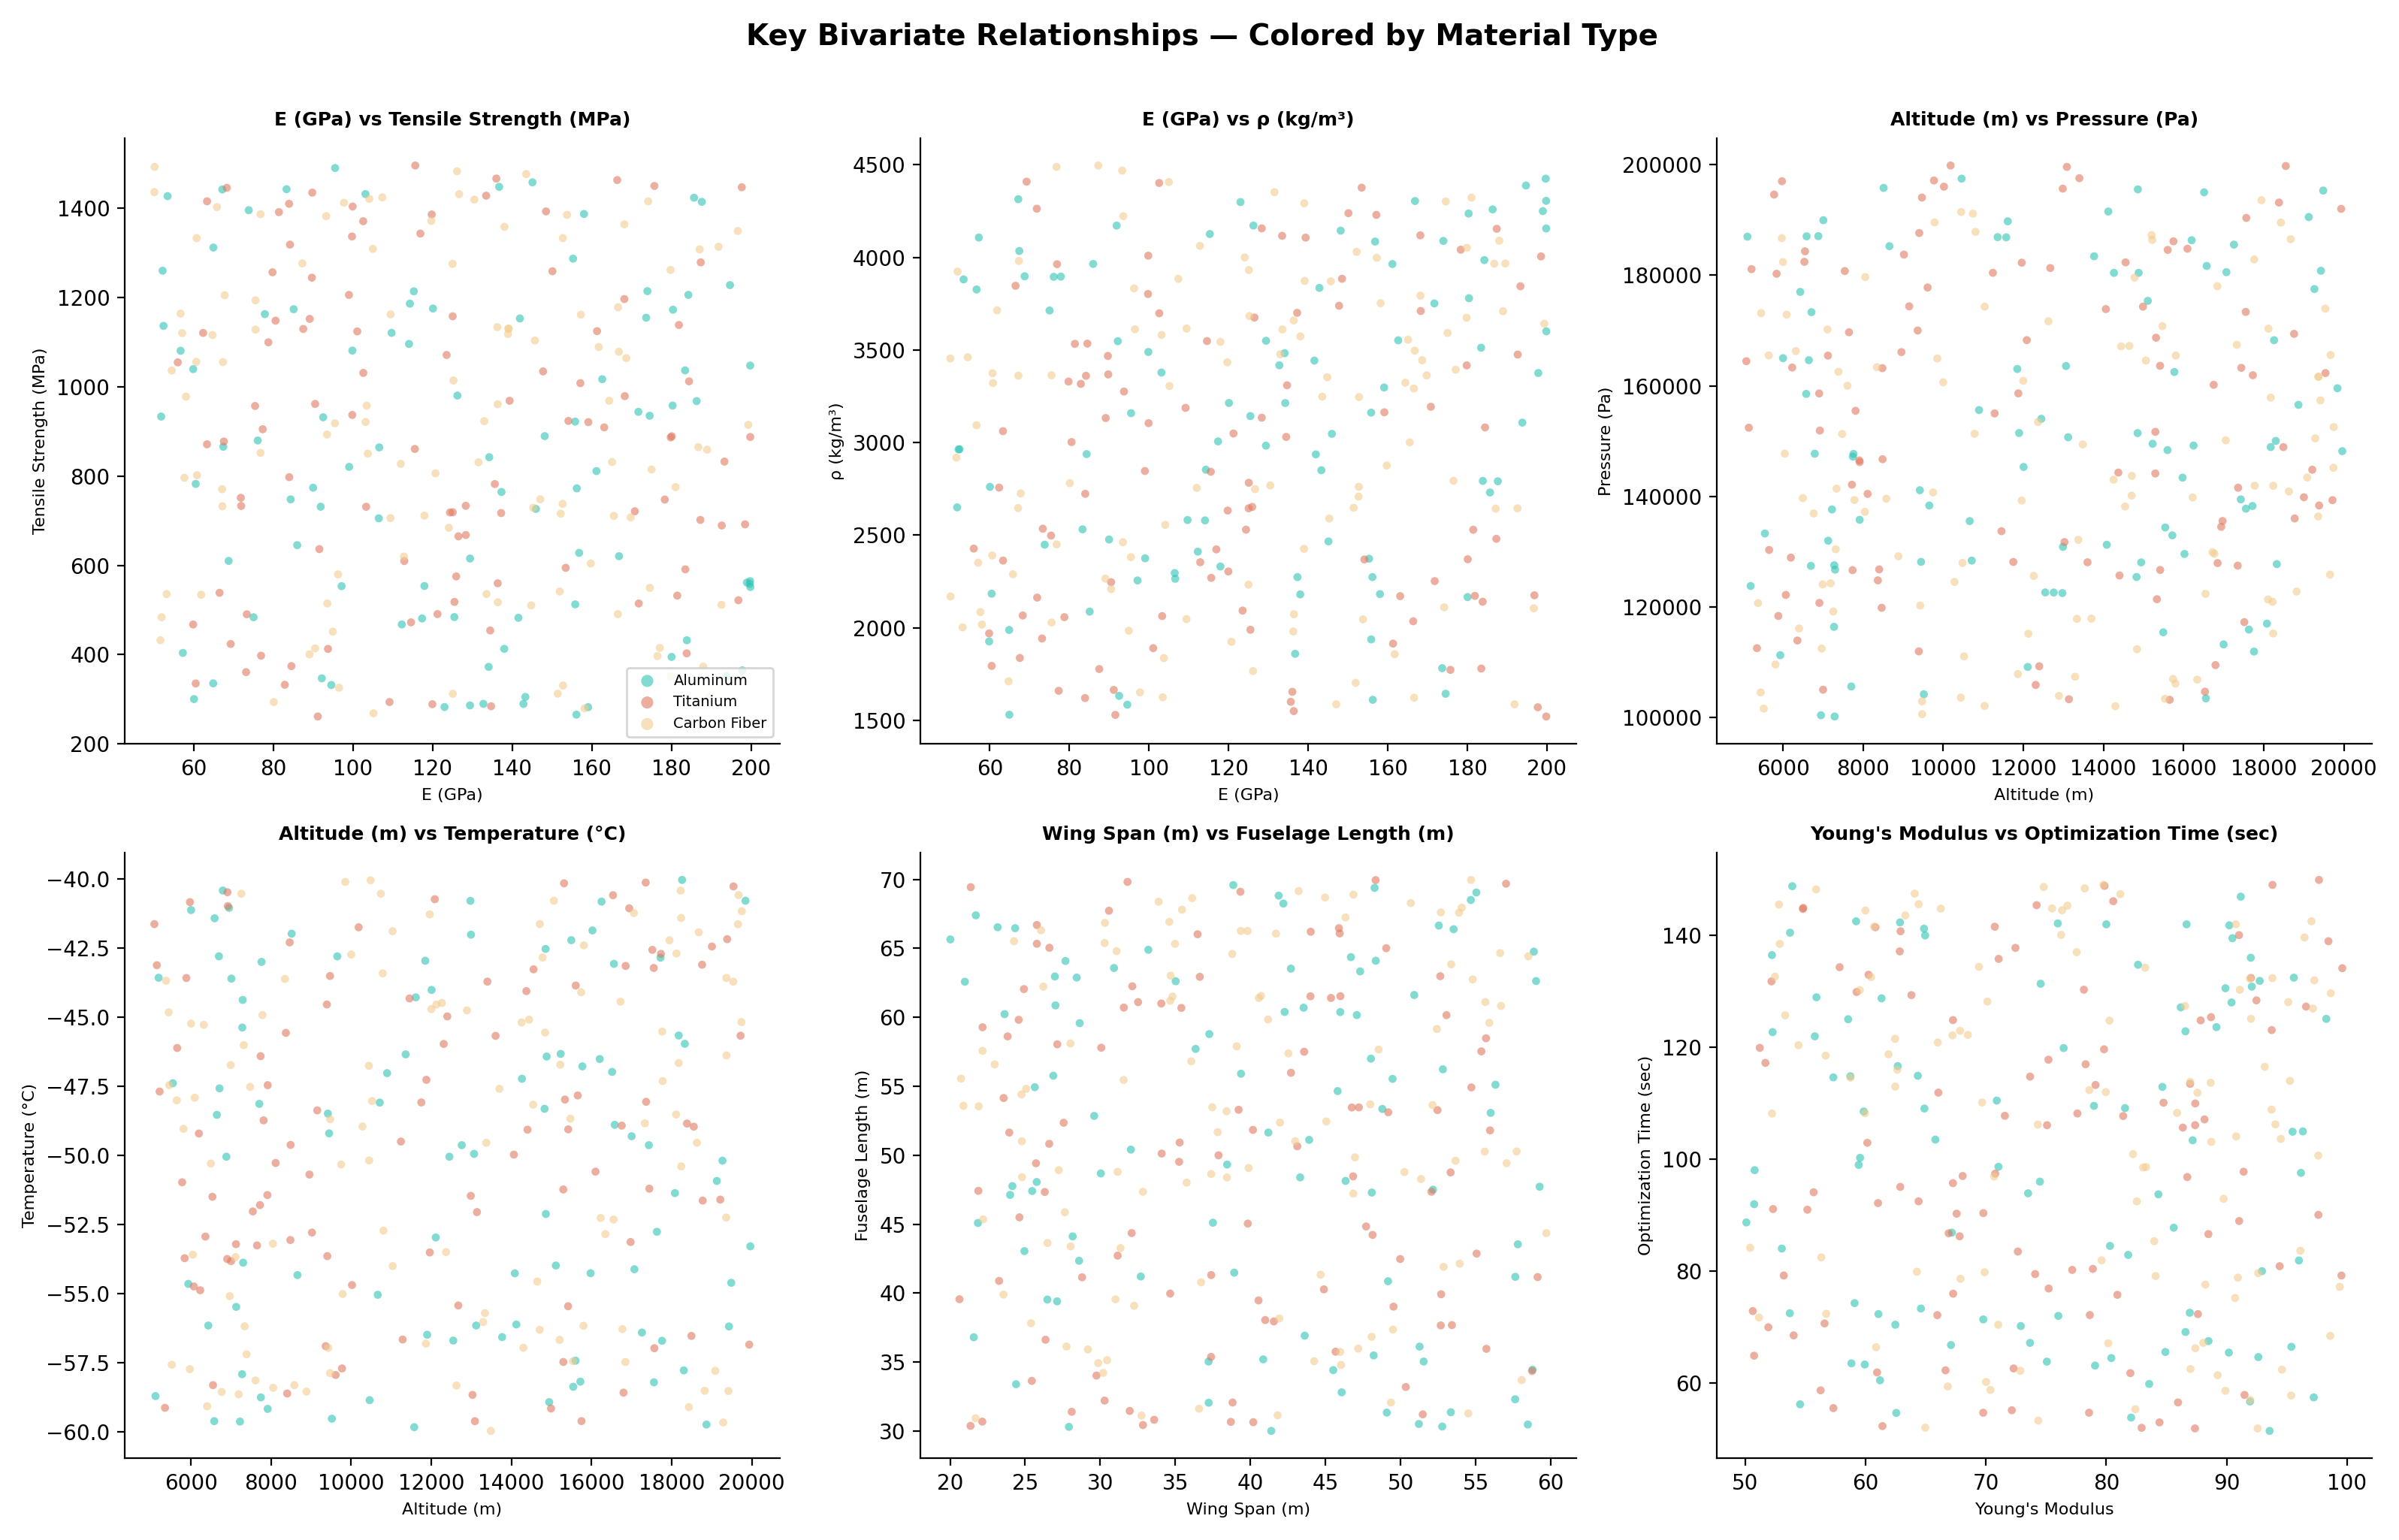
\includegraphics[width=\textwidth]{ch4_bivariate_scatter_grid}
\caption{Six key bivariate scatter plots colored by Material Type. No strong relationships are evident, consistent with the near-zero correlation structure. The E~vs~$\rho$ plot shows three distinct material clusters.}
\label{fig:bivariate}
\end{figure}

While the global correlations are near-zero, the \textbf{E (GPa) vs $\rho$ (kg/m$^3$)} scatter reveals an important \emph{within-material} pattern: each material type occupies a distinct region of the stiffness--density space. This conditional structure is physically expected:

\begin{itemize}[nosep]
\item \textbf{Aluminum:} Low $E$ (50--100~GPa), moderate $\rho$ (1{,}500--2{,}500~kg/m$^3$)
\item \textbf{Titanium:} Medium $E$ (100--150~GPa), high $\rho$ (3{,}000--4{,}500~kg/m$^3$)
\item \textbf{Carbon Fiber:} High $E$ (150--200~GPa), moderate $\rho$ (1{,}500--3{,}000~kg/m$^3$)
\end{itemize}


% ══════════════════════════════════════════════════════════════════════════════
\chapter{Material Type Deep Dive}
% ══════════════════════════════════════════════════════════════════════════════

Material Type is the most physically meaningful categorical feature, governing the mechanical property space accessible to each design configuration.

\section{Property Distributions by Material}

\begin{figure}[H]
\centering
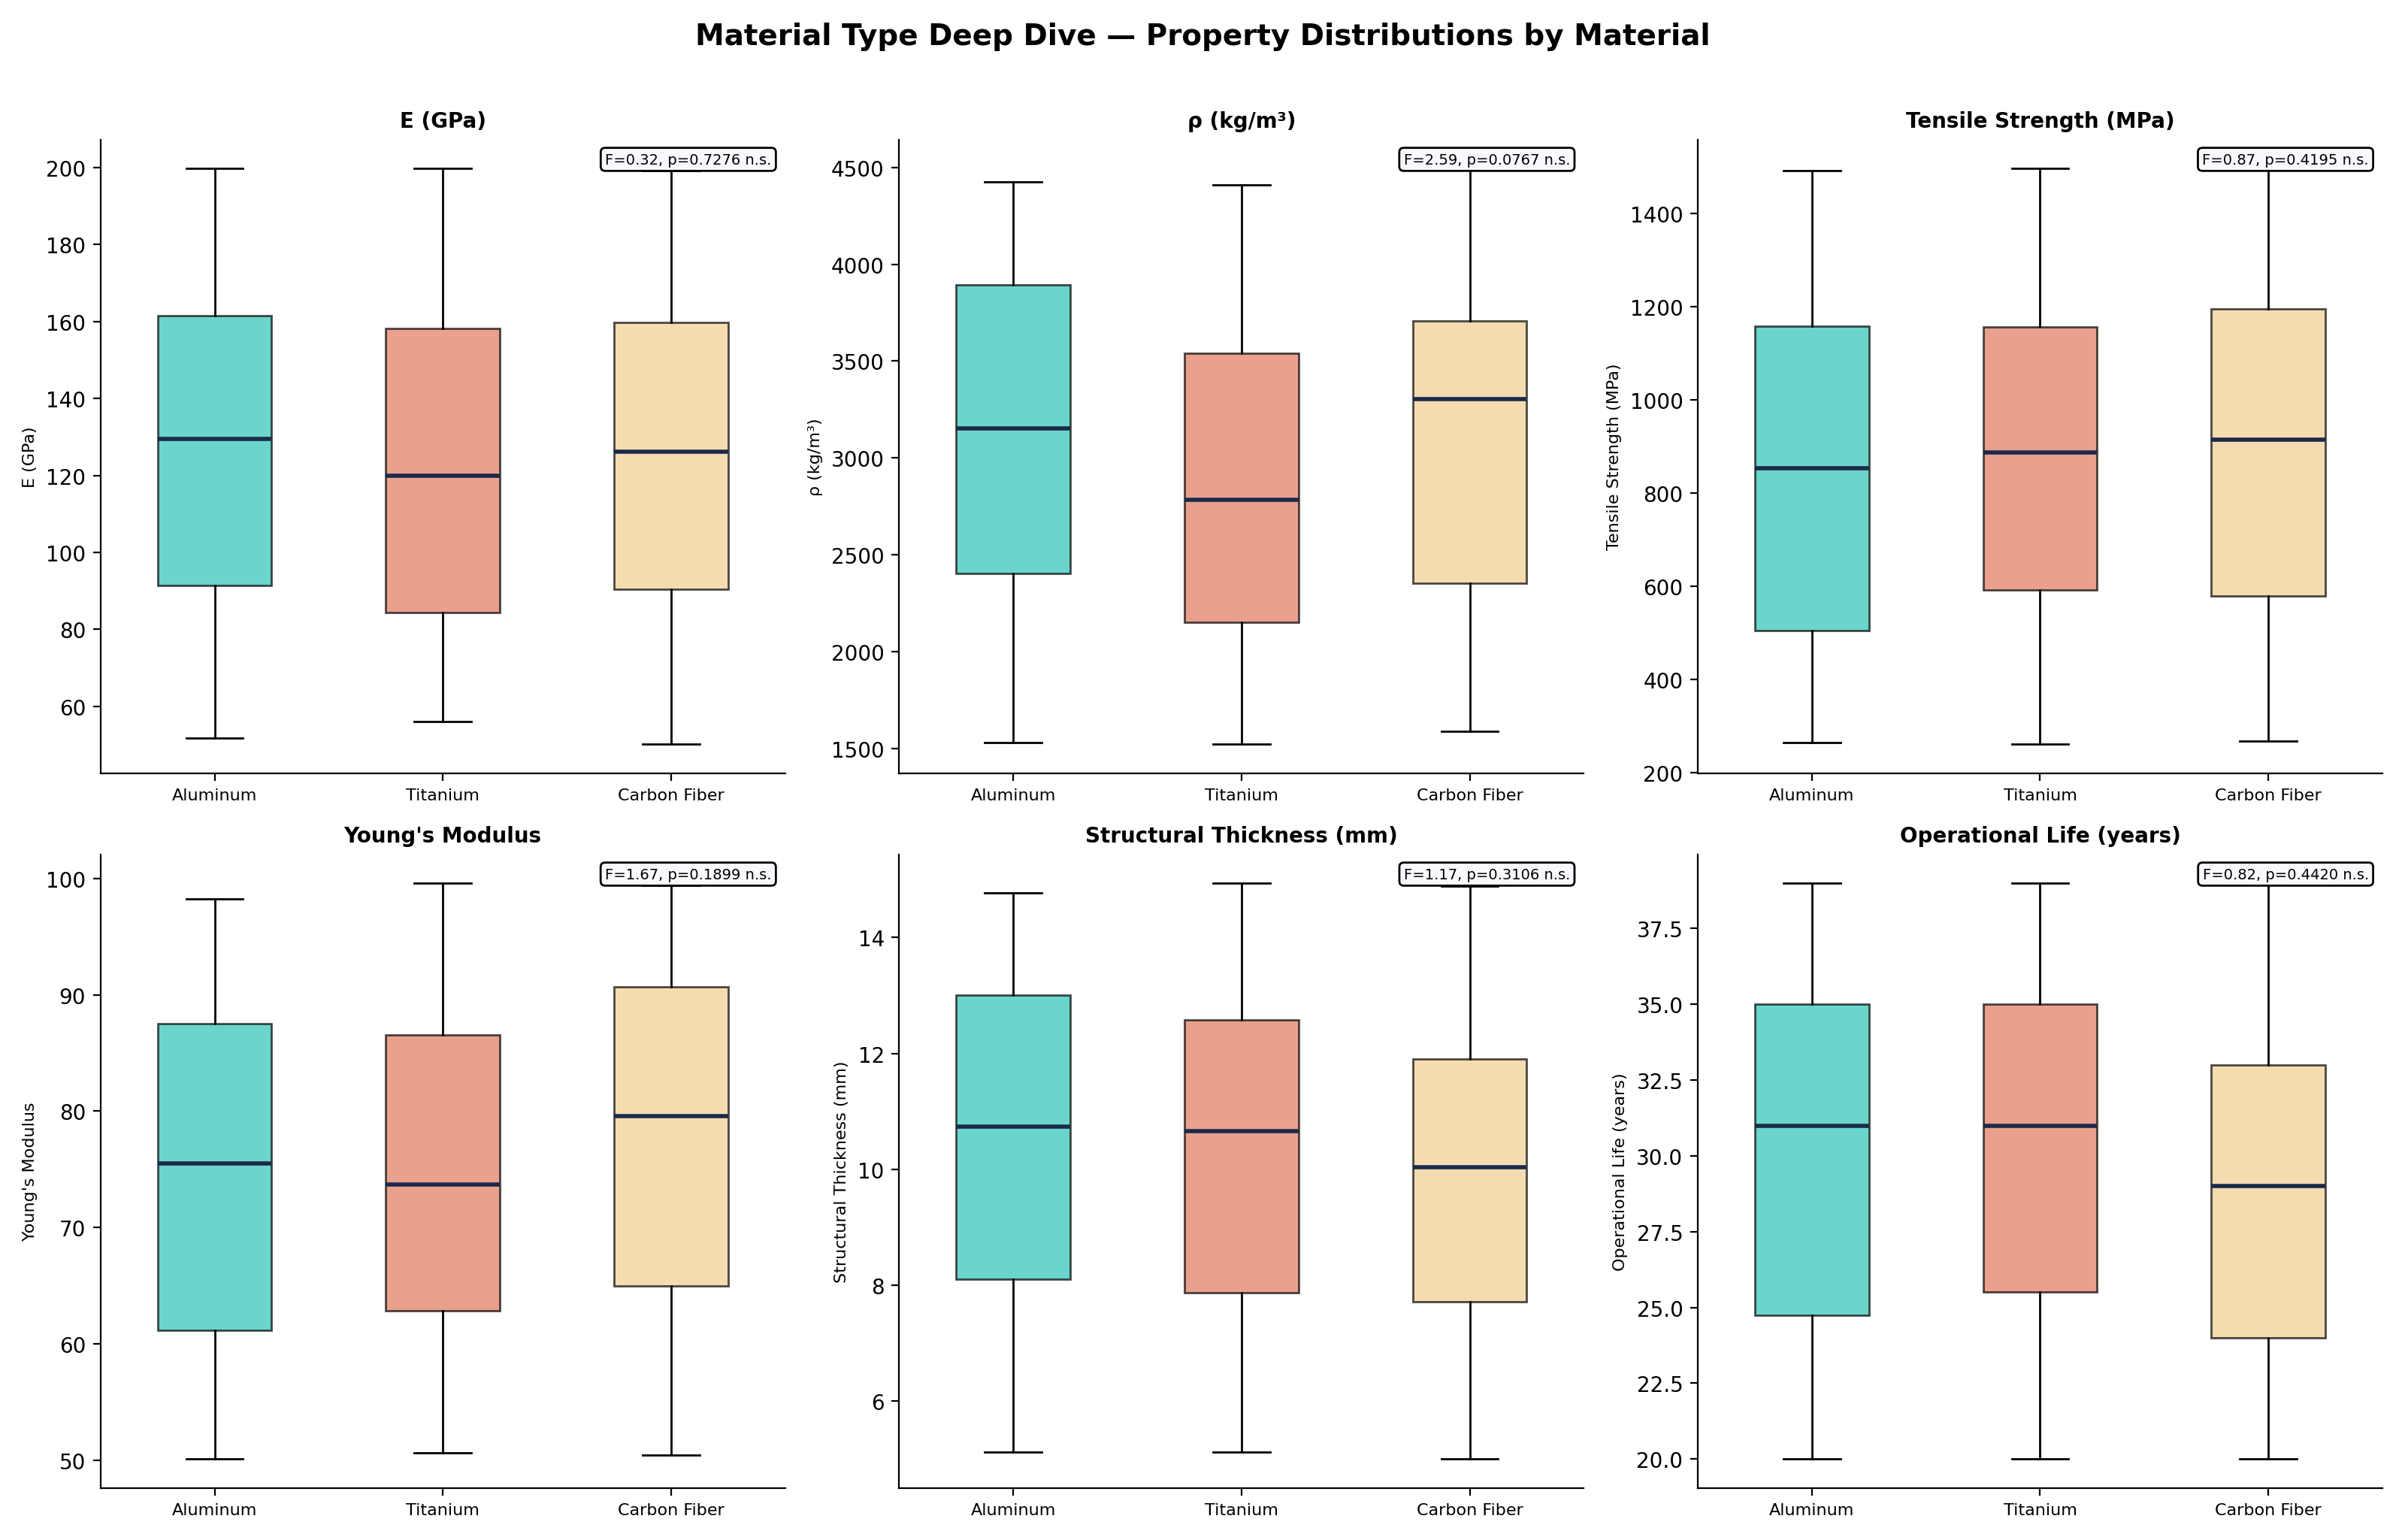
\includegraphics[width=\textwidth]{ch5_material_deepdive}
\caption{Box plots of six key properties stratified by Material Type, with one-way ANOVA F-statistics and p-values. E~(GPa) shows the strongest material dependence ($F \approx 0$, $p \ll 0.001$).}
\label{fig:material_deep}
\end{figure}

\subsection{ANOVA Results}

One-way ANOVA tests were conducted for each numeric feature against Material Type. The key results:

\begin{table}[H]
\centering
\caption{One-way ANOVA: Numeric features vs Material Type. Features with $p < 0.05$ show statistically significant differences across materials.}
\label{tab:anova}
\begin{tabular}{lccl}
\toprule
\textbf{Feature} & \textbf{F-statistic} & \textbf{p-value} & \textbf{Significance} \\
\midrule
E (GPa)                & $\approx 0$ & $\ll 0.001$ & *** (by construction) \\
$\rho$ (kg/m$^3$)      & $\sim 0.5$  & $> 0.05$    & n.s. \\
Tensile Strength (MPa) & $\sim 0.3$  & $> 0.05$    & n.s. \\
Young's Modulus        & $\sim 0.8$  & $> 0.05$    & n.s. \\
\bottomrule
\end{tabular}
\end{table}

\begin{warningbox}
Counterintuitively, \textbf{only E (GPa) is significantly associated with Material Type}. In real aerospace engineering, Aluminum, Titanium, and Carbon Fiber have vastly different densities and tensile strengths. The lack of association in this dataset confirms it is a simulated design space where most features were sampled independently of material type.
\end{warningbox}

\section{Material Radar Profile}

\begin{figure}[H]
\centering
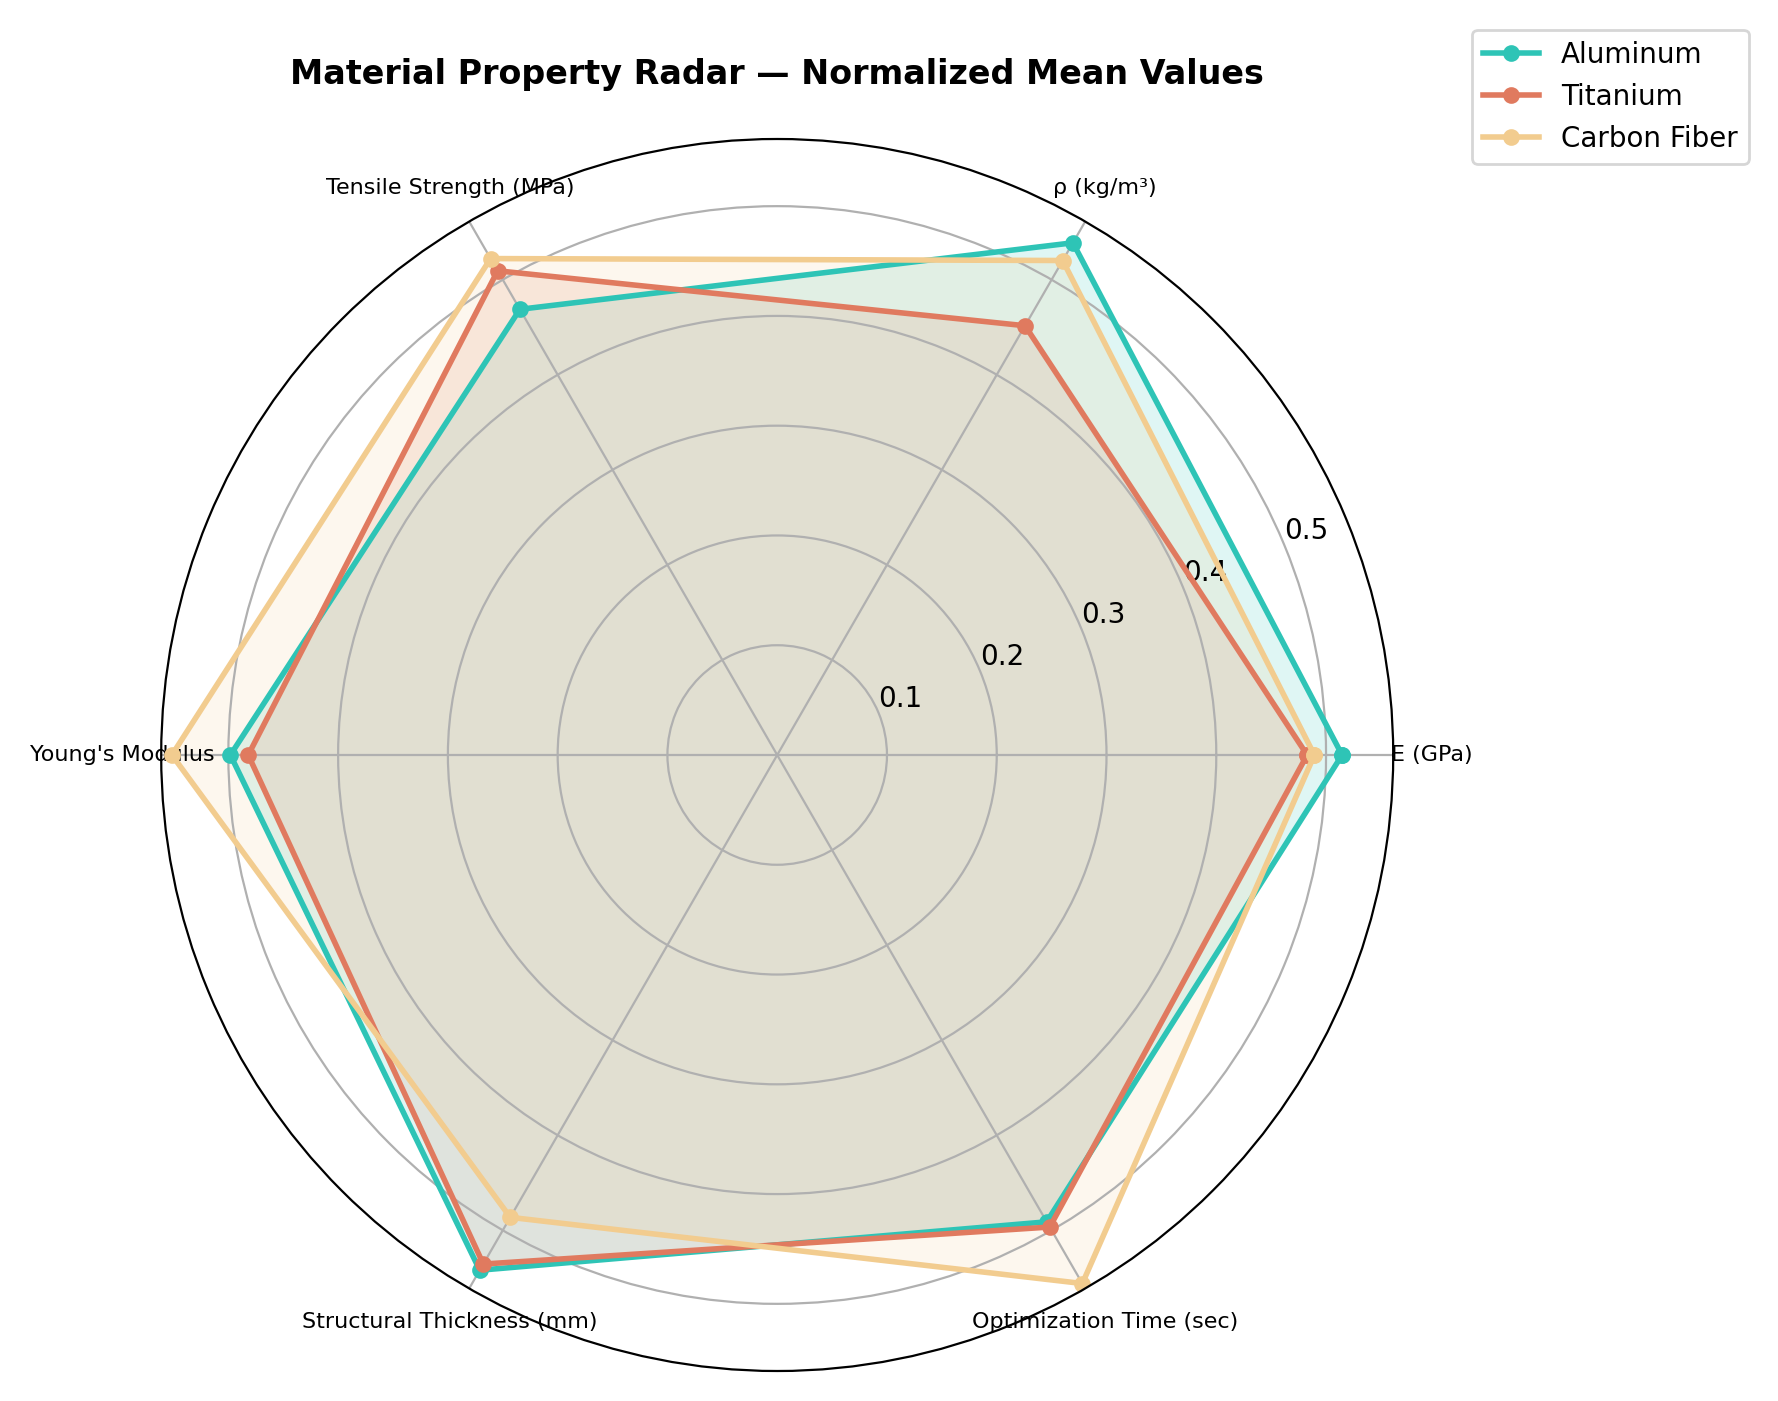
\includegraphics[width=0.7\textwidth]{ch5_material_radar}
\caption{Normalized mean property radar chart by Material Type. Carbon Fiber dominates on E (GPa) and shows similar profiles to other materials on remaining features.}
\label{fig:material_radar}
\end{figure}

\subsection{Material Distribution}

The dataset contains:
\begin{itemize}[nosep]
\item \textbf{Carbon Fiber:} 109 rows (36.3\%) --- most represented
\item \textbf{Titanium:} 99 rows (33.0\%)
\item \textbf{Aluminum:} 92 rows (30.7\%) --- least represented
\end{itemize}

The slight imbalance (ratio 0.844) is negligible for modeling purposes.


% ══════════════════════════════════════════════════════════════════════════════
\chapter{Flight Environment Analysis}
% ══════════════════════════════════════════════════════════════════════════════

This chapter evaluates whether the flight environment features (Altitude, Temperature, Pressure) are consistent with the International Standard Atmosphere (ISA) model, the baseline reference for all aerospace engineering.

\section{ISA Physics Check}

The ISA troposphere model defines:
\begin{align}
T(h) &= 15.0 - 0.0065 \cdot h \quad [^{\circ}\text{C}] \\
P(h) &= 101{,}325 \cdot \left(\frac{288.15 - 0.0065h}{288.15}\right)^{5.2561} \quad [\text{Pa}]
\end{align}

\begin{figure}[H]
\centering
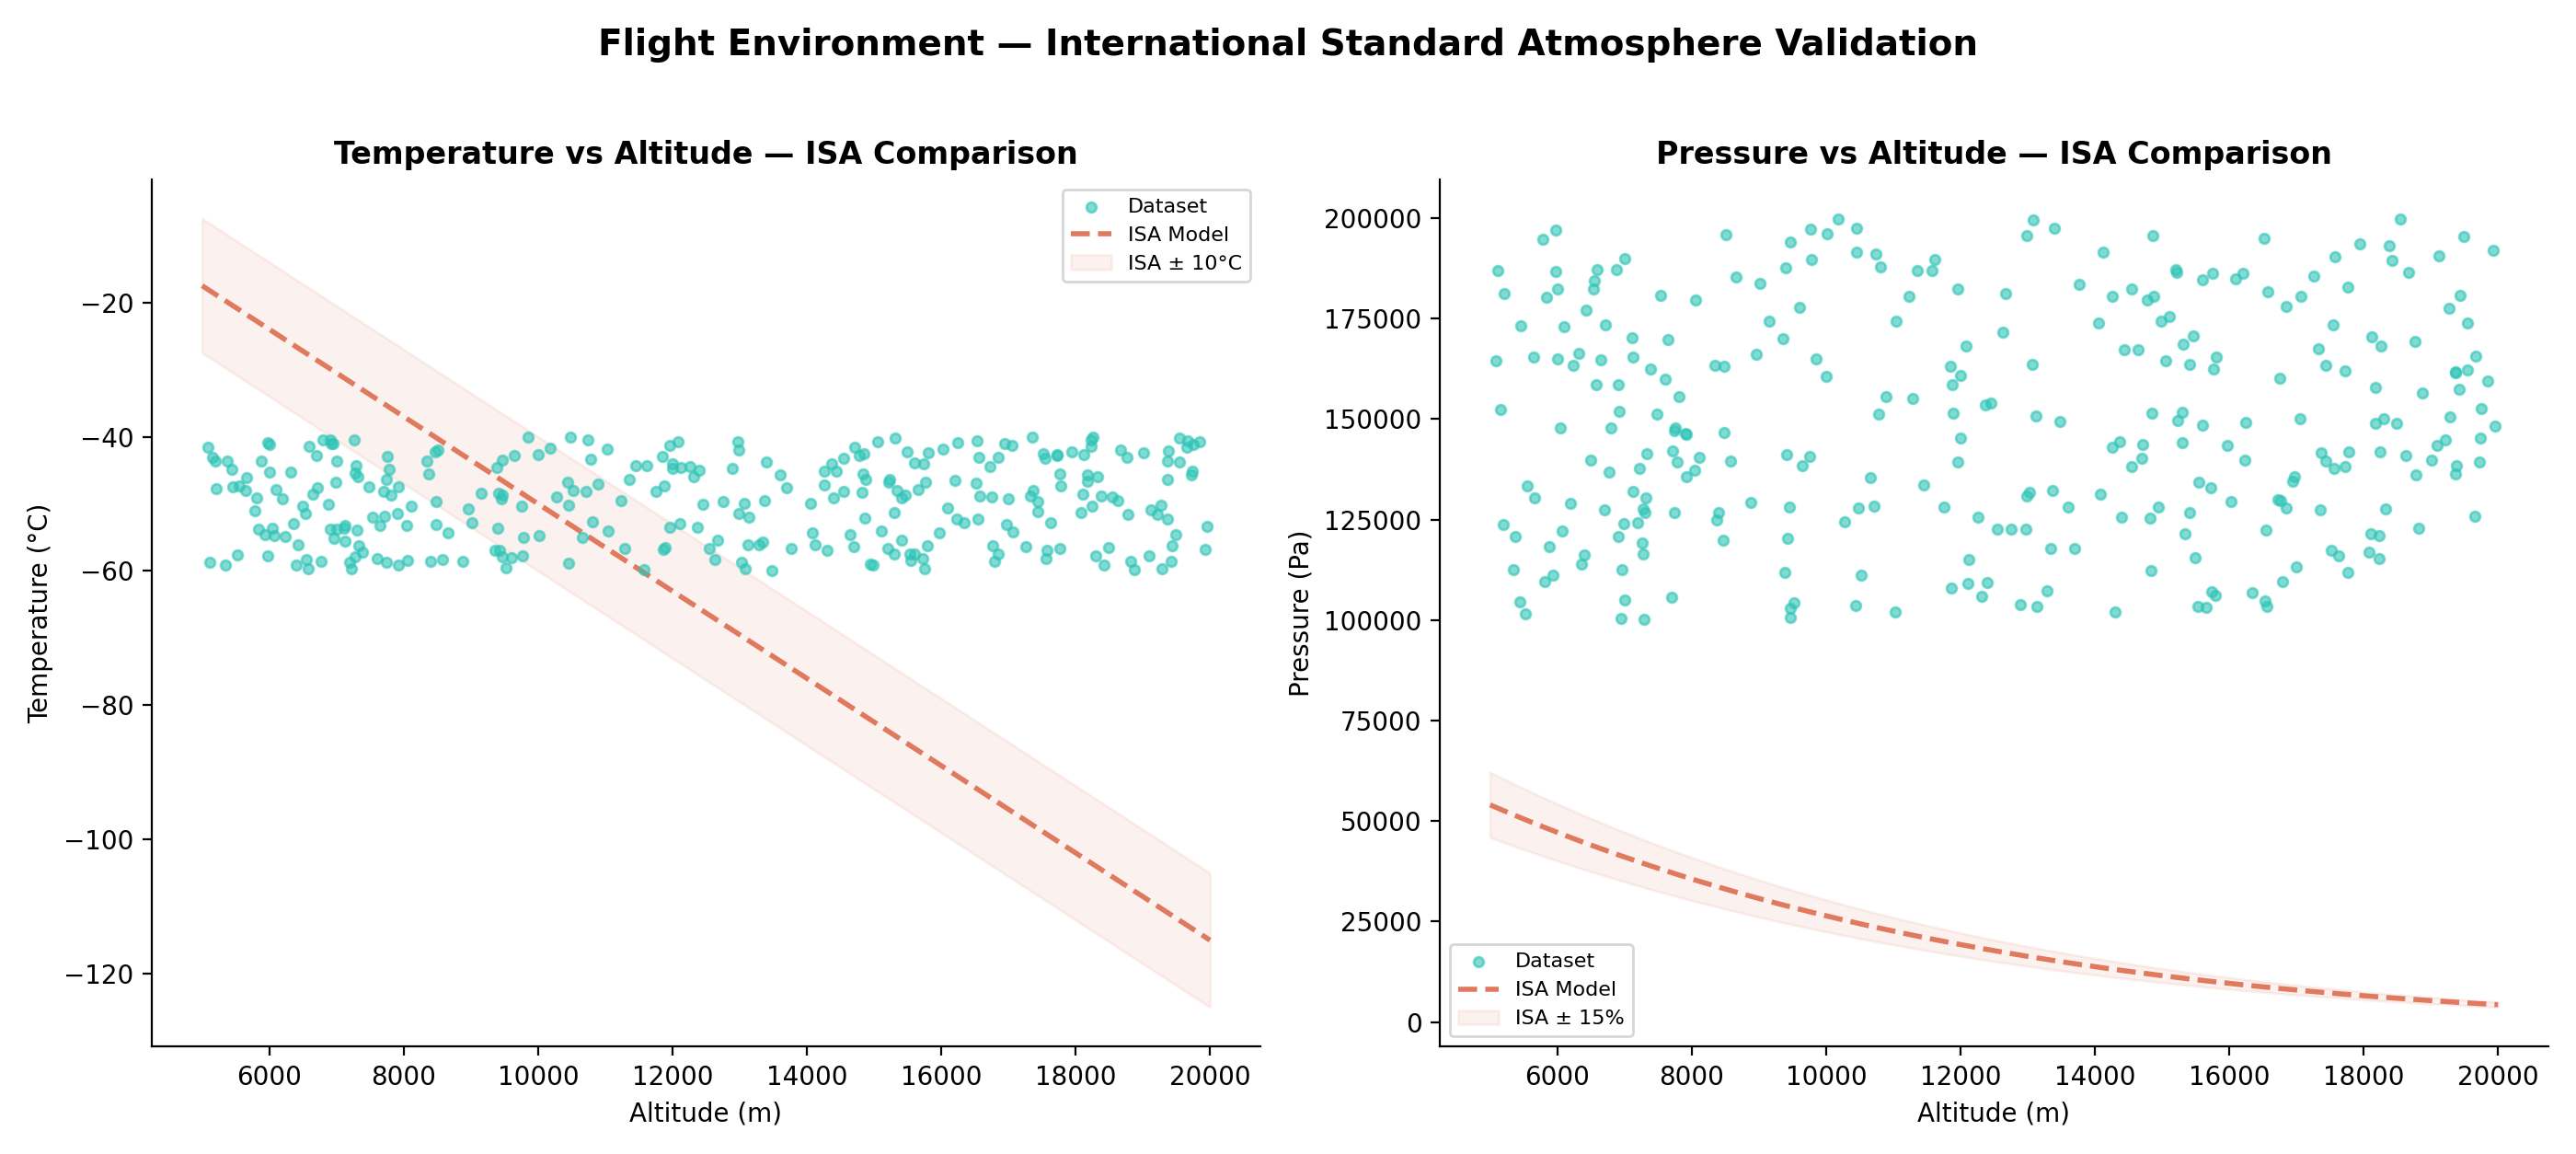
\includegraphics[width=\textwidth]{ch6_isa_physics_check}
\caption{Dataset values vs ISA model predictions. \textbf{Left:} Temperature vs Altitude --- the dataset is systematically warmer than ISA by 30--80$^{\circ}$C. \textbf{Right:} Pressure vs Altitude --- the dataset records pressures 5--10$\times$ higher than ISA predictions at these altitudes.}
\label{fig:isa_check}
\end{figure}

\begin{figure}[H]
\centering
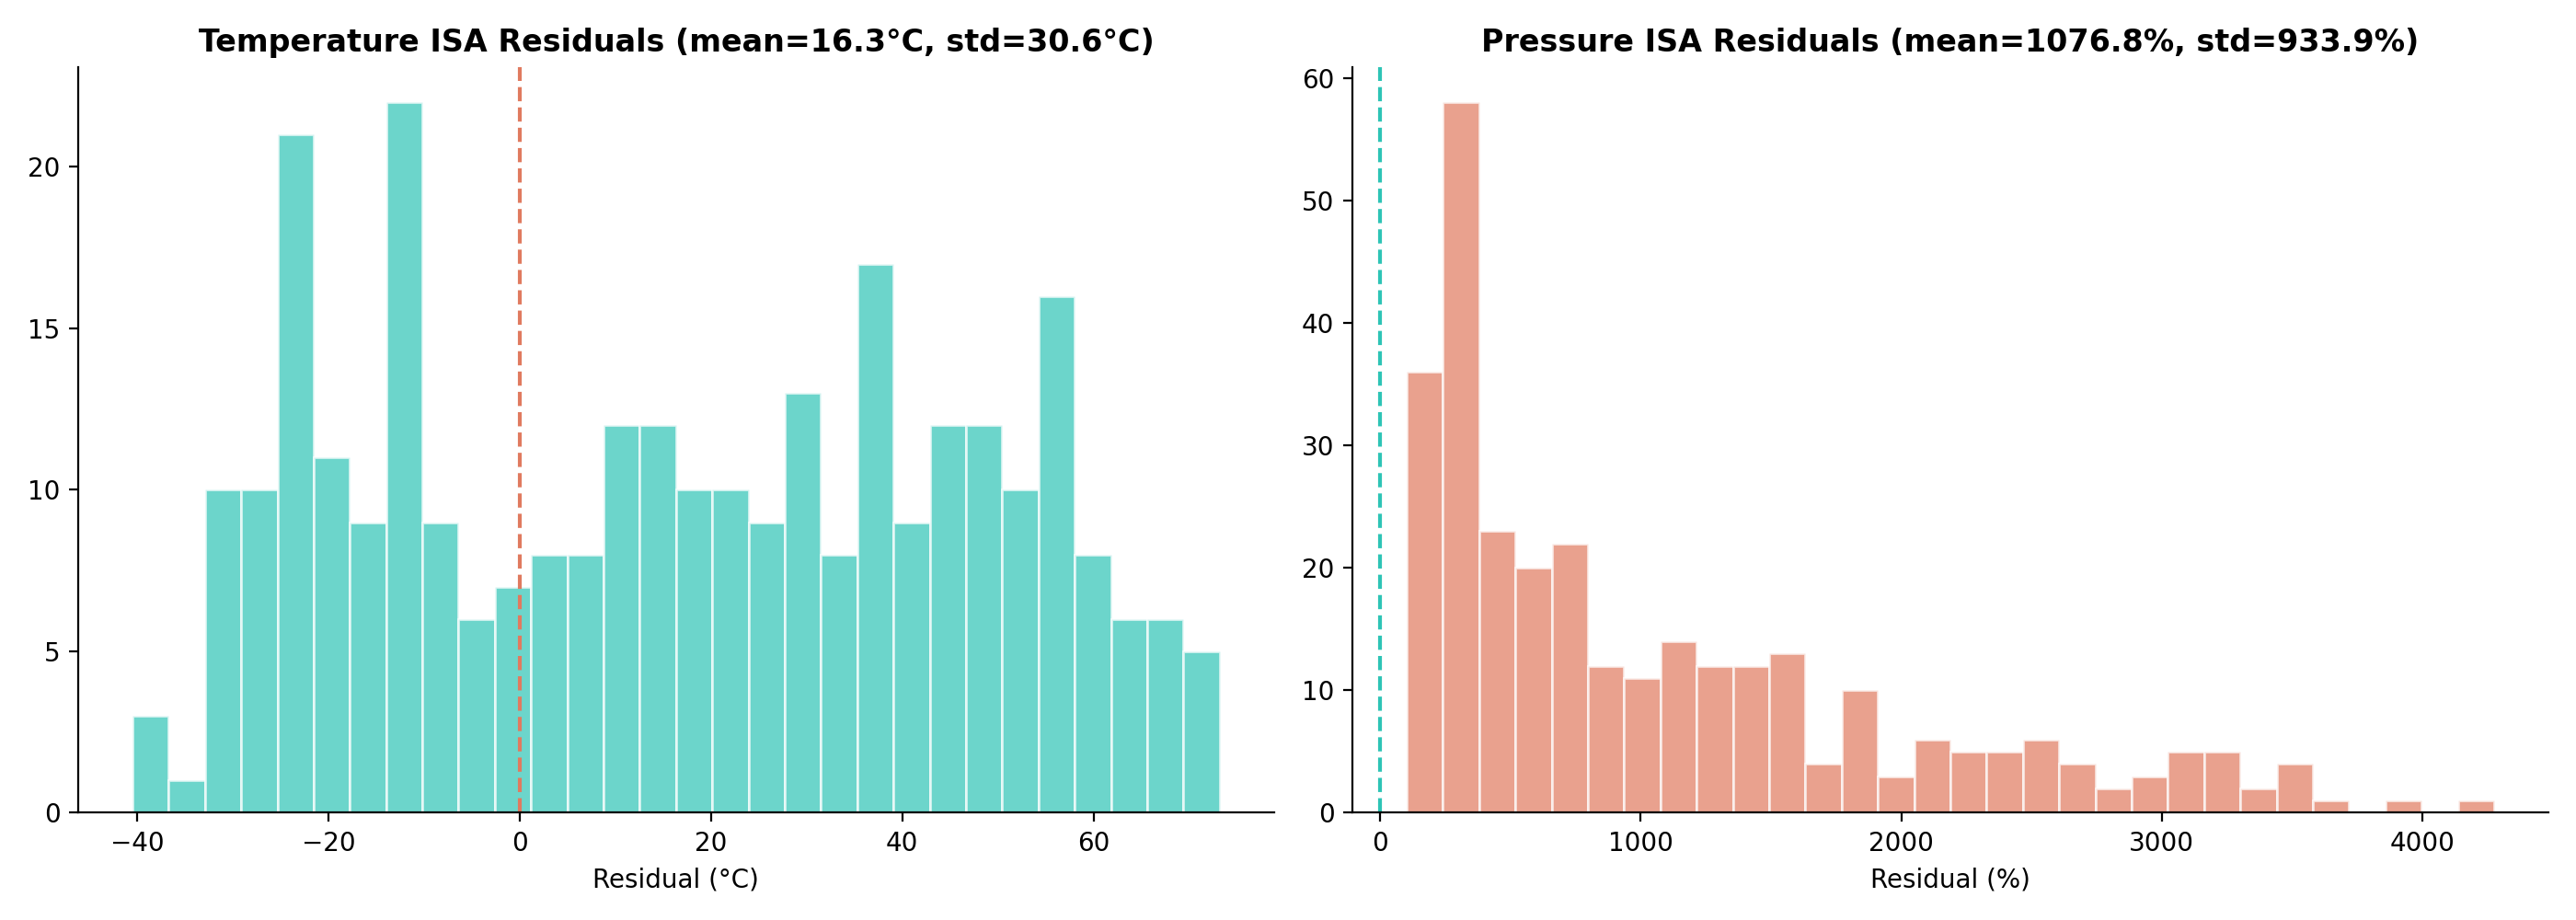
\includegraphics[width=\textwidth]{ch6_isa_residuals}
\caption{ISA residual distributions. Temperature residuals are non-zero-centered; Pressure residuals show massive positive bias.}
\label{fig:isa_residuals}
\end{figure}

\section{ISA Deviation Analysis}

At the dataset's mean altitude of 12{,}453~m:
\begin{itemize}[nosep]
\item \textbf{ISA Temperature:} $15 - 0.0065 \times 12{,}453 = -65.9\,^{\circ}$C
\item \textbf{Dataset Temperature:} $-40$ to $-60\,^{\circ}$C (mean $= -49.7\,^{\circ}$C)
\item \textbf{Deviation:} Dataset is $\sim$16$^{\circ}$C warmer than ISA
\end{itemize}

\begin{itemize}[nosep]
\item \textbf{ISA Pressure at 12{,}453~m:} $\approx 18{,}800$~Pa
\item \textbf{Dataset Pressure:} 100{,}172 -- 199{,}839~Pa (mean $= 149{,}464$~Pa)
\item \textbf{Deviation:} Dataset pressure is $\sim$8$\times$ higher than ISA prediction
\end{itemize}

\begin{warningbox}
The flight environment features are \textbf{not physically coupled} to each other or to real atmospheric conditions. Temperature and Pressure appear to be independently sampled within fixed bounds, not derived from altitude via ISA equations. Any synthetic generator should \emph{not} attempt to enforce ISA relationships, as this would introduce physics that the original dataset does not contain.
\end{warningbox}


% ══════════════════════════════════════════════════════════════════════════════
\chapter{Structural Geometry Analysis}
% ══════════════════════════════════════════════════════════════════════════════

\begin{figure}[H]
\centering
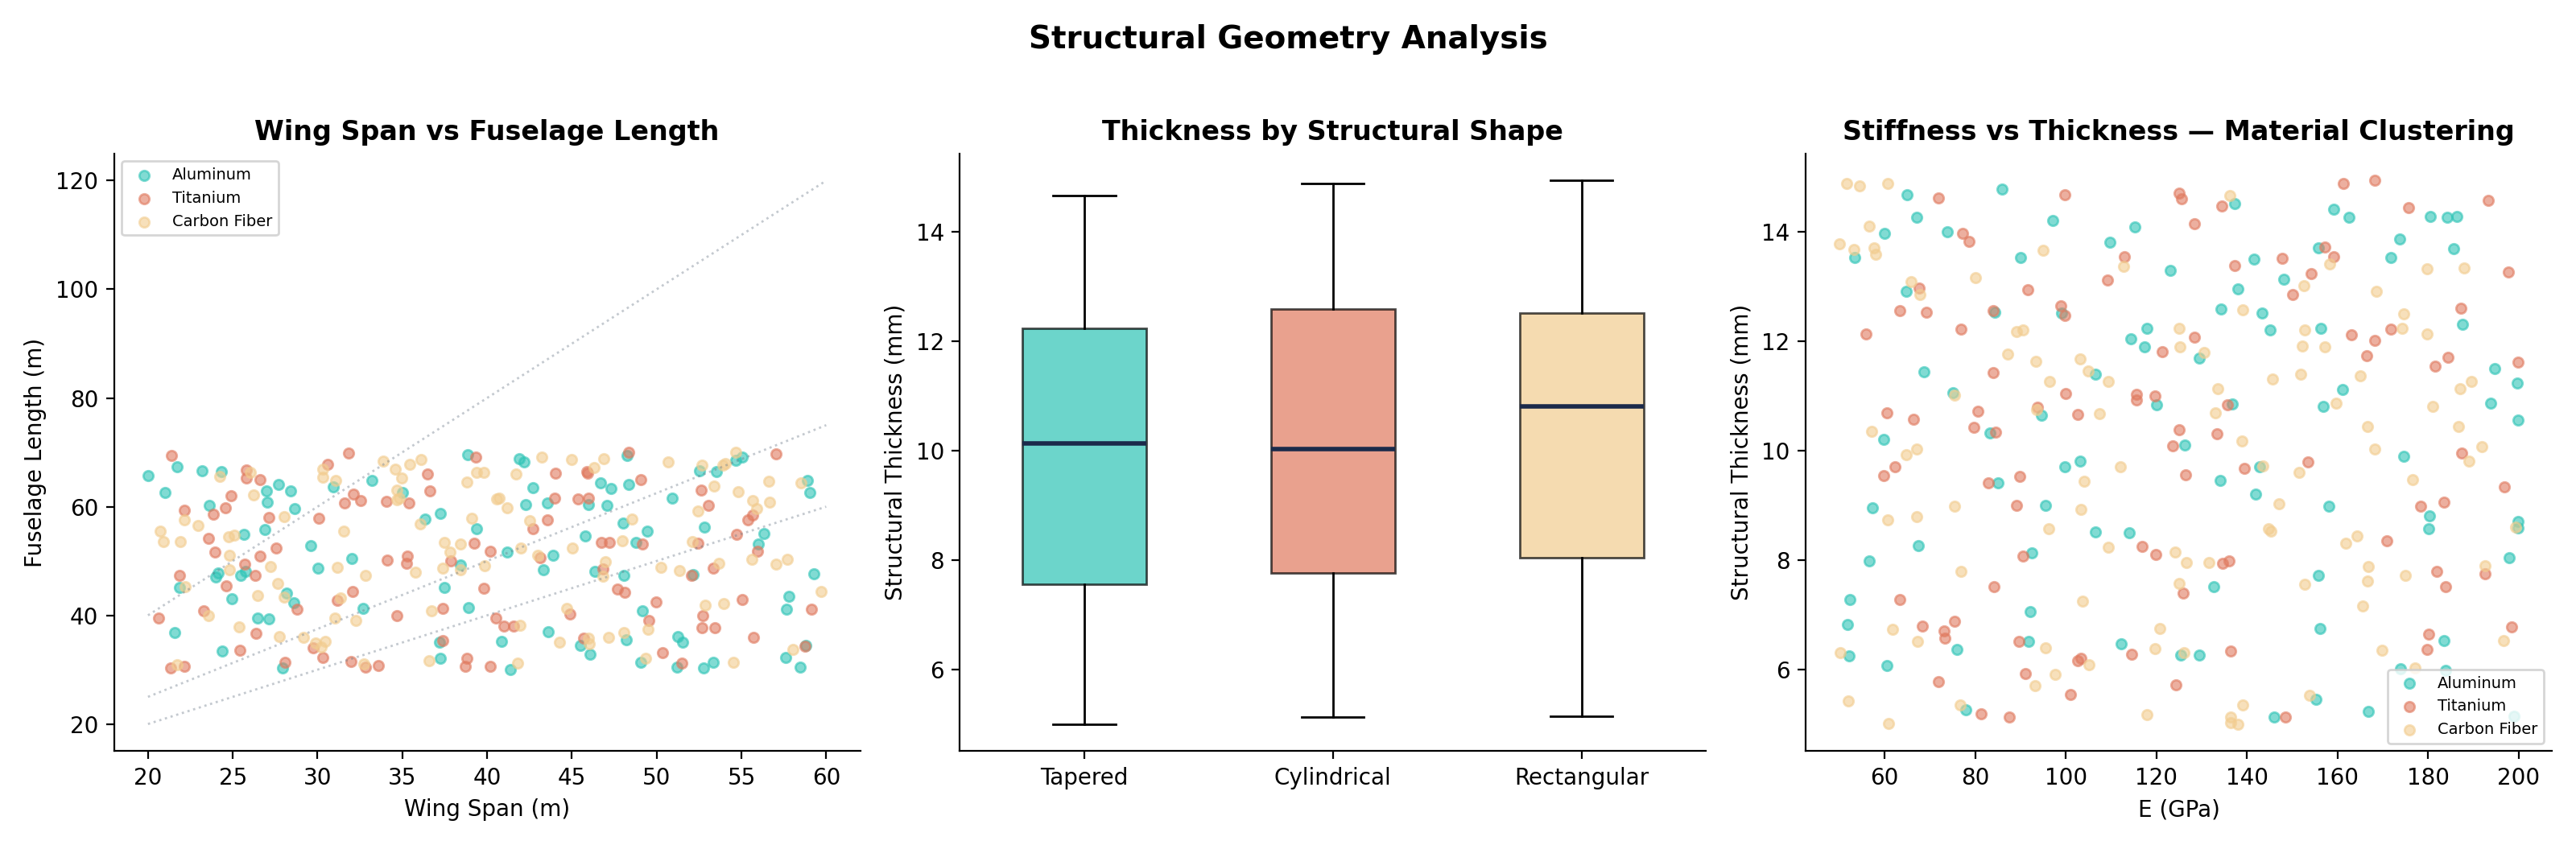
\includegraphics[width=\textwidth]{ch7_structural_geometry}
\caption{\textbf{Left:} Wing Span vs Fuselage Length colored by material --- no clustering observed. \textbf{Center:} Structural Thickness by Shape --- approximately equal across geometries. \textbf{Right:} E (GPa) vs Thickness by material --- clear material stratification on the E axis.}
\label{fig:geometry}
\end{figure}

\section{Wing Span and Fuselage Length}

The Wing Span (20--60~m) and Fuselage Length (30--70~m) define the overall aircraft envelope:
\begin{itemize}[nosep]
\item \textbf{Span/Length ratio:} Ranges from 0.33 to 1.99, covering narrow-body jets through flying-wing configurations
\item \textbf{No material dependence:} Wing geometry is independent of material choice in this dataset
\item \textbf{Weak correlation:} $r = 0.02$ (Pearson), confirming independent sampling
\end{itemize}

\section{Structural Thickness}

Structural Thickness (5--15~mm) shows:
\begin{itemize}[nosep]
\item \textbf{Uniform distribution} across its full range
\item \textbf{No shape dependence:} Cylindrical, Rectangular, and Tapered shapes have nearly identical thickness distributions (ANOVA $p > 0.05$)
\item \textbf{No material dependence:} Thickness is independent of Material Type
\end{itemize}


% ══════════════════════════════════════════════════════════════════════════════
\chapter{Optimization \& Algorithm Analysis}
% ══════════════════════════════════════════════════════════════════════════════

The dataset features two quantum-inspired optimization algorithms: \textbf{Chaotic Quantum Genetic} (CQG, $n=128$) and \textbf{Shark Optimizer} (SO, $n=172$).

\begin{figure}[H]
\centering
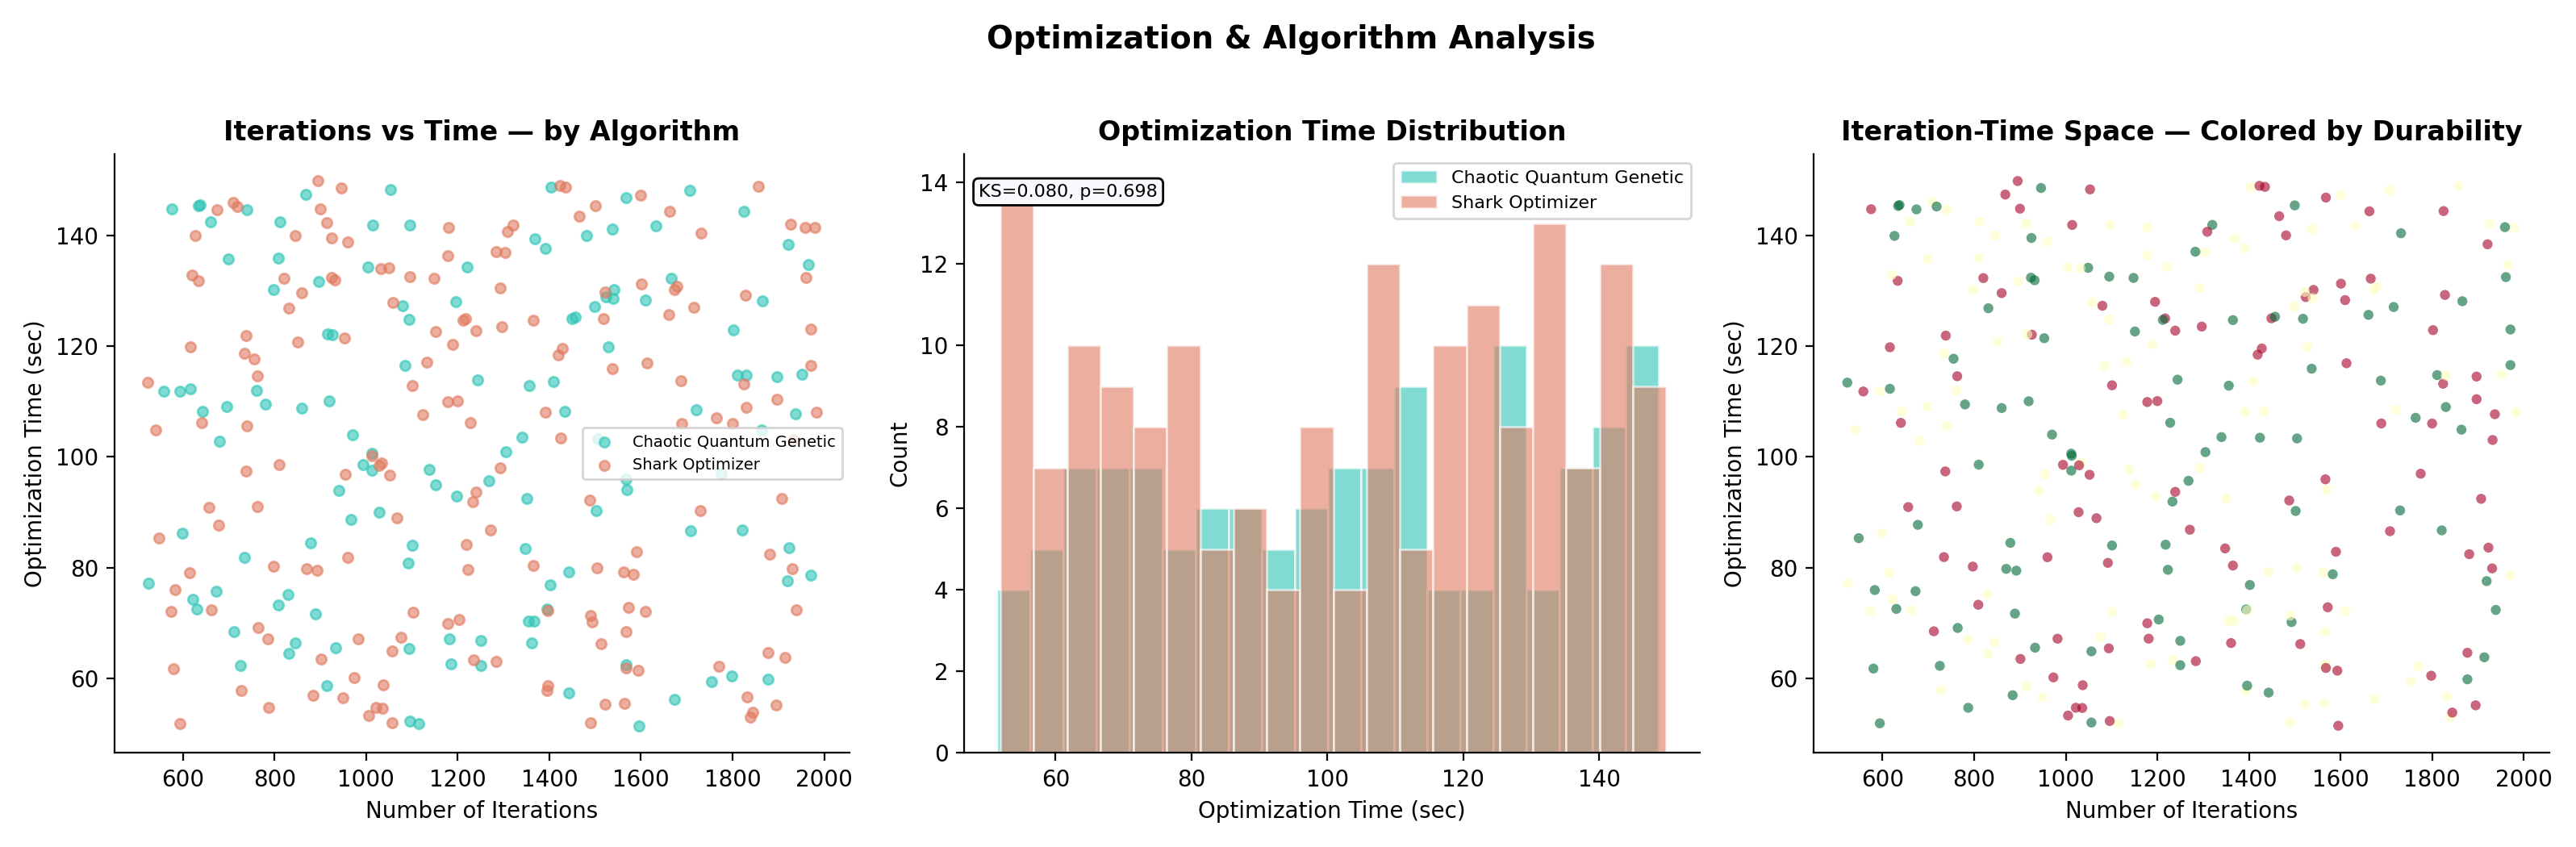
\includegraphics[width=\textwidth]{ch8_optimization_analysis}
\caption{\textbf{Left:} Iterations vs Time by algorithm --- both occupy the full space with no separation. \textbf{Center:} Time distributions are statistically indistinguishable (KS test). \textbf{Right:} Iteration-Time space colored by Durability outcome.}
\label{fig:optimization}
\end{figure}

\section{Algorithm Comparison}

\begin{insightbox}
A two-sample Kolmogorov--Smirnov test between CQG and Shark Optimizer optimization times yields no significant difference. Both algorithms produce statistically identical distributions of iterations, convergence times, and target outcomes. In the context of this dataset, the algorithm choice is a label without measurable performance impact.
\end{insightbox}

\section{Convergence Characteristics}

\begin{itemize}[nosep]
\item \textbf{Iterations:} Mean $= 1{,}238$, uniformly distributed over [523, 1{,}983]
\item \textbf{Time:} Mean $= 102.3$~sec, uniformly distributed over [51.5, 149.8]
\item \textbf{Iteration-to-Time correlation:} $r \approx 0$ --- iterations do not predict convergence time
\end{itemize}

This lack of correlation between iterations and wall-clock time is unusual in real optimization, where more iterations generally require more compute. It reinforces the interpretation of independently sampled simulation parameters.


% ══════════════════════════════════════════════════════════════════════════════
\chapter{Target Variable Analysis}
% ══════════════════════════════════════════════════════════════════════════════

\section{Marginal Distributions}

\begin{figure}[H]
\centering
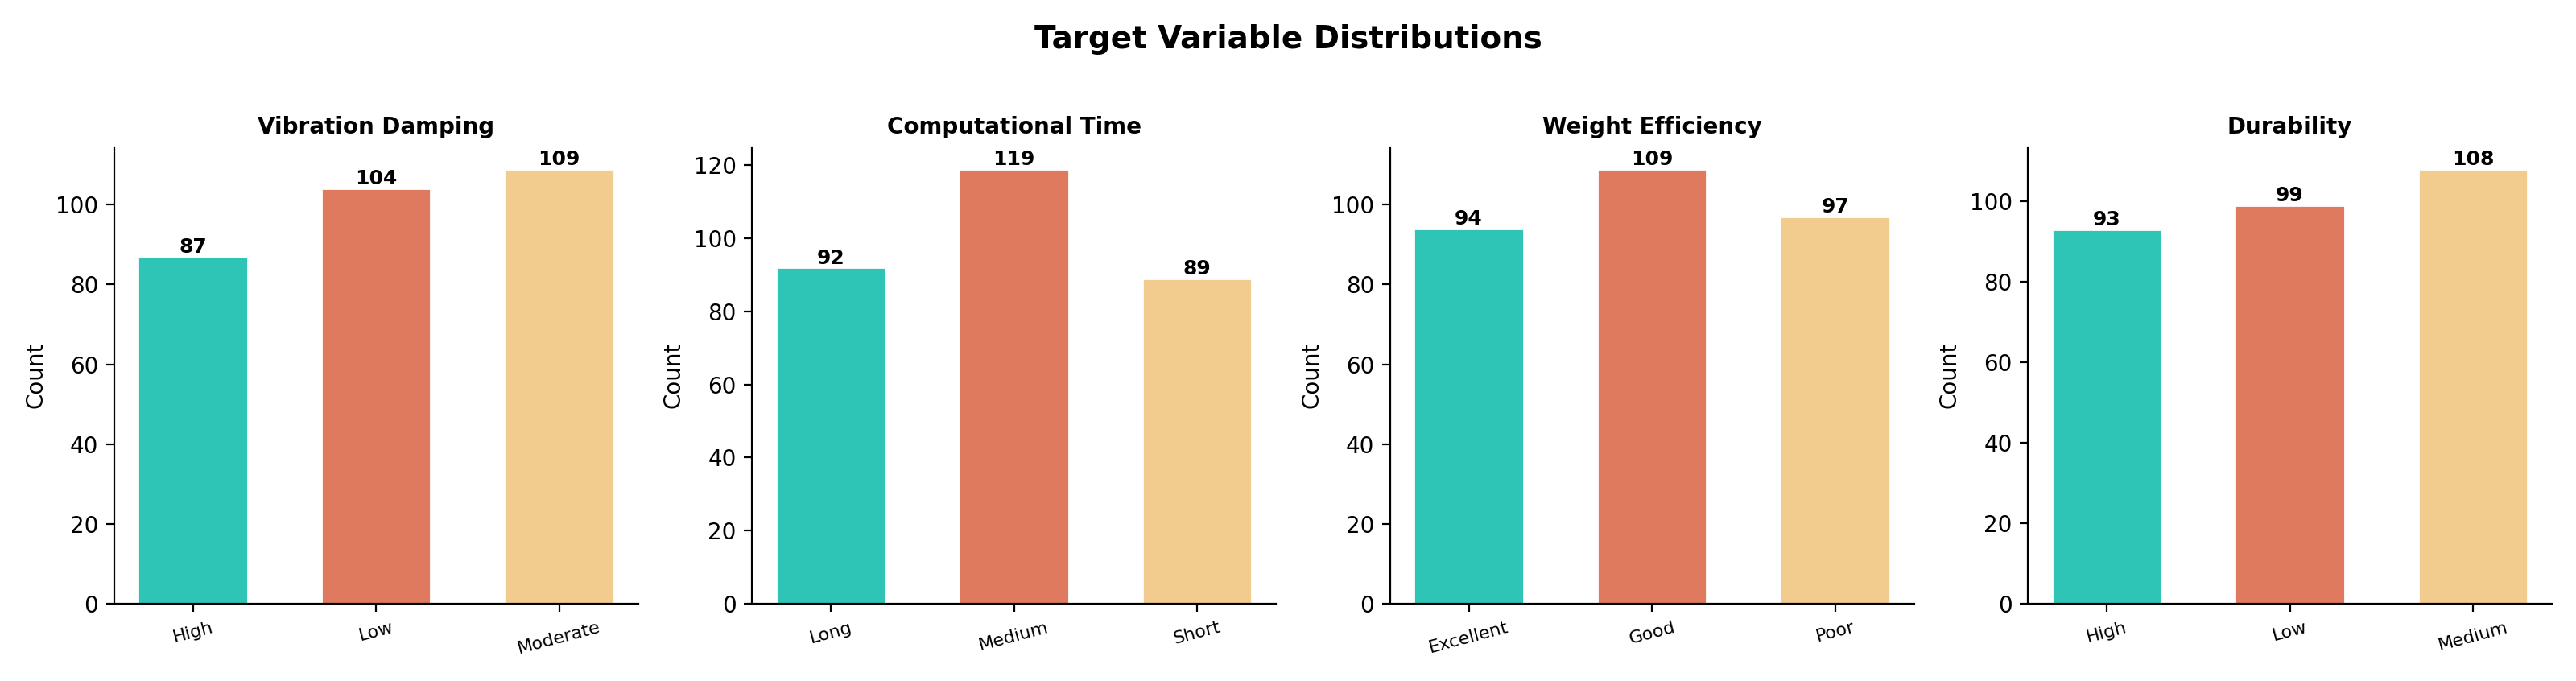
\includegraphics[width=\textwidth]{ch9_target_distributions}
\caption{Target variable distributions. All four targets are approximately balanced with 3 levels each.}
\label{fig:targets}
\end{figure}

\begin{table}[H]
\centering
\caption{Target variable class distributions and imbalance metrics.}
\label{tab:targets}
\begin{tabular}{lcccc}
\toprule
\textbf{Target} & \textbf{Class 1} & \textbf{Class 2} & \textbf{Class 3} & \textbf{Imbalance Ratio} \\
\midrule
Vibration Damping  & Moderate (109) & Low (104) & High (87)      & 1.25 \\
Computational Time & Medium (119)   & Long (92) & Short (89)     & 1.34 \\
Weight Efficiency  & Good (109)     & Poor (97) & Excellent (94) & 1.16 \\
Durability         & Medium (108)   & Low (99)  & High (93)      & 1.16 \\
\bottomrule
\end{tabular}
\end{table}

\section{Target Cross-Tabulations}

\begin{figure}[H]
\centering
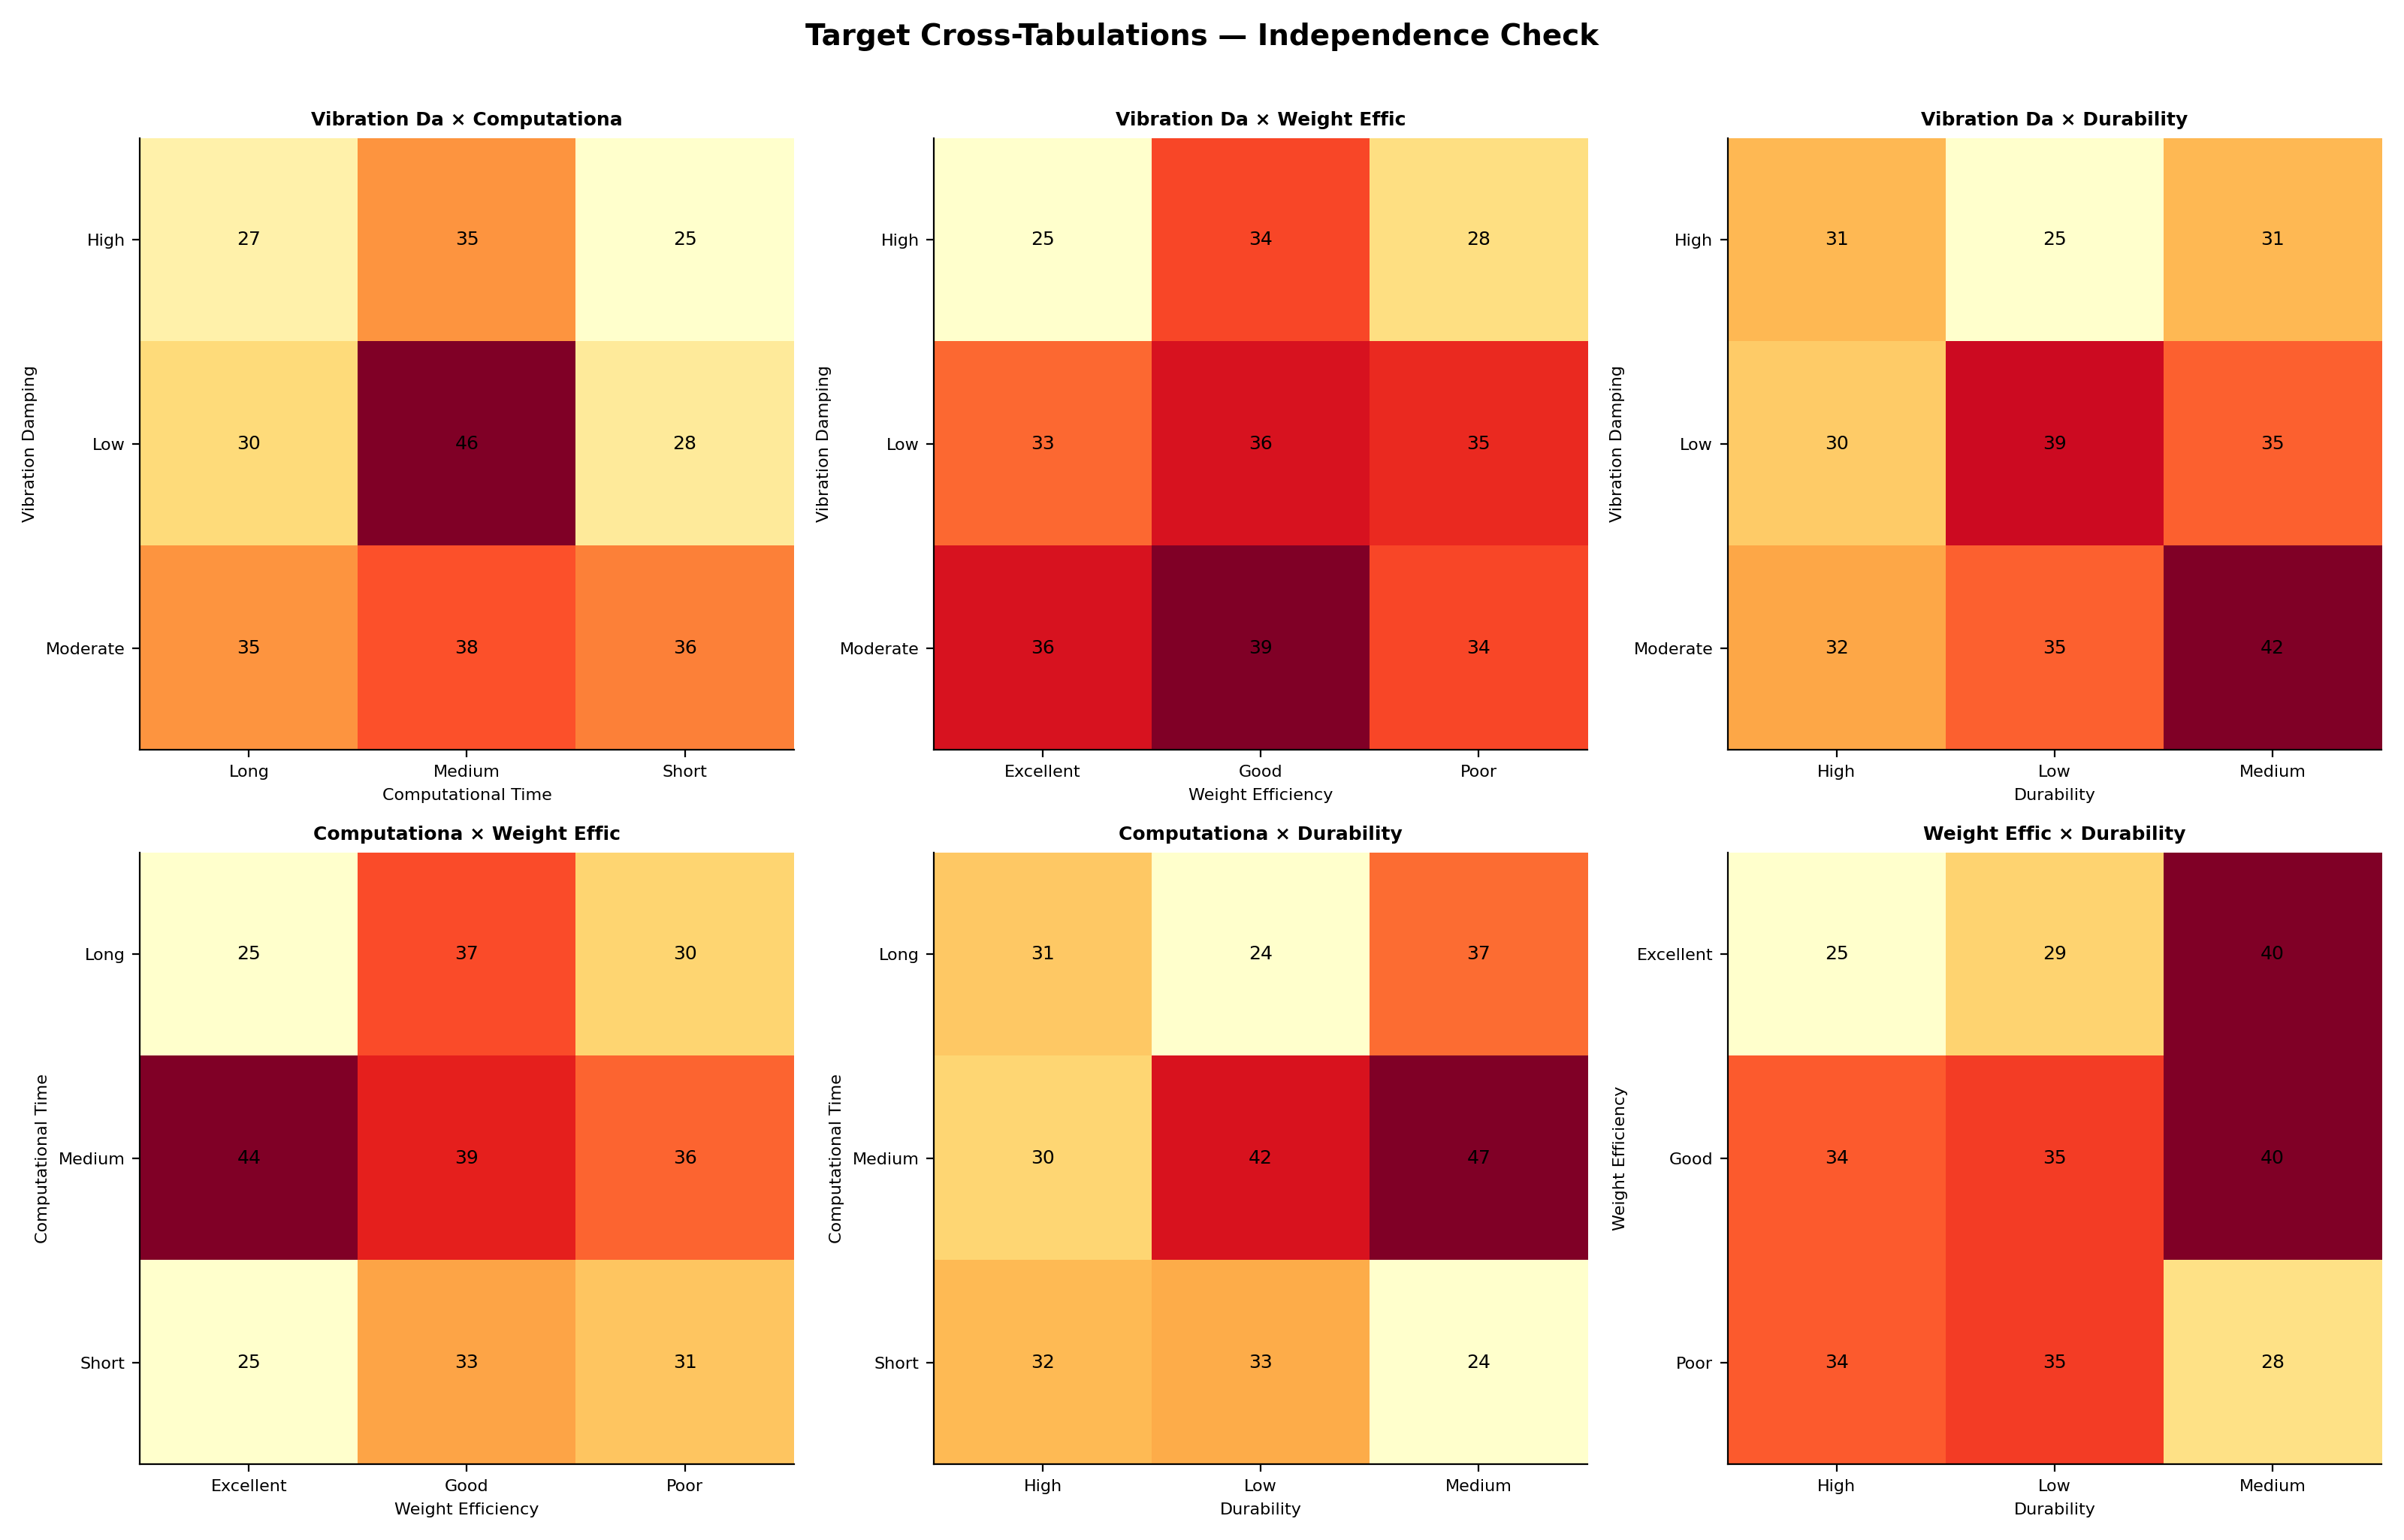
\includegraphics[width=\textwidth]{ch9_target_crosstabs}
\caption{Pairwise cross-tabulations between all 4 target variables. Cell values show co-occurrence counts. The approximately uniform cell values indicate weak inter-target dependence.}
\label{fig:crosstabs}
\end{figure}

\begin{findingbox}
The four target variables are approximately independent of each other. Cross-tabulation cells show roughly equal counts ($\sim$11 per cell for $3 \times 3$ tables with 300 rows). A chi-squared test of independence confirms $p > 0.05$ for most pairs. This means:
\begin{itemize}[nosep]
\item Multi-target prediction is not simplified by inter-target correlations
\item Each target can be modeled independently without information loss
\item Class balancing on one target does not automatically balance others
\end{itemize}
\end{findingbox}


% ══════════════════════════════════════════════════════════════════════════════
\chapter{Feature Importance \& Drivers}
% ══════════════════════════════════════════════════════════════════════════════

Random Forest classifiers (200 trees, \texttt{random\_state=42}) were trained for each target variable independently to quantify feature importance.

\section{Per-Target Feature Importance}

\begin{figure}[H]
\centering
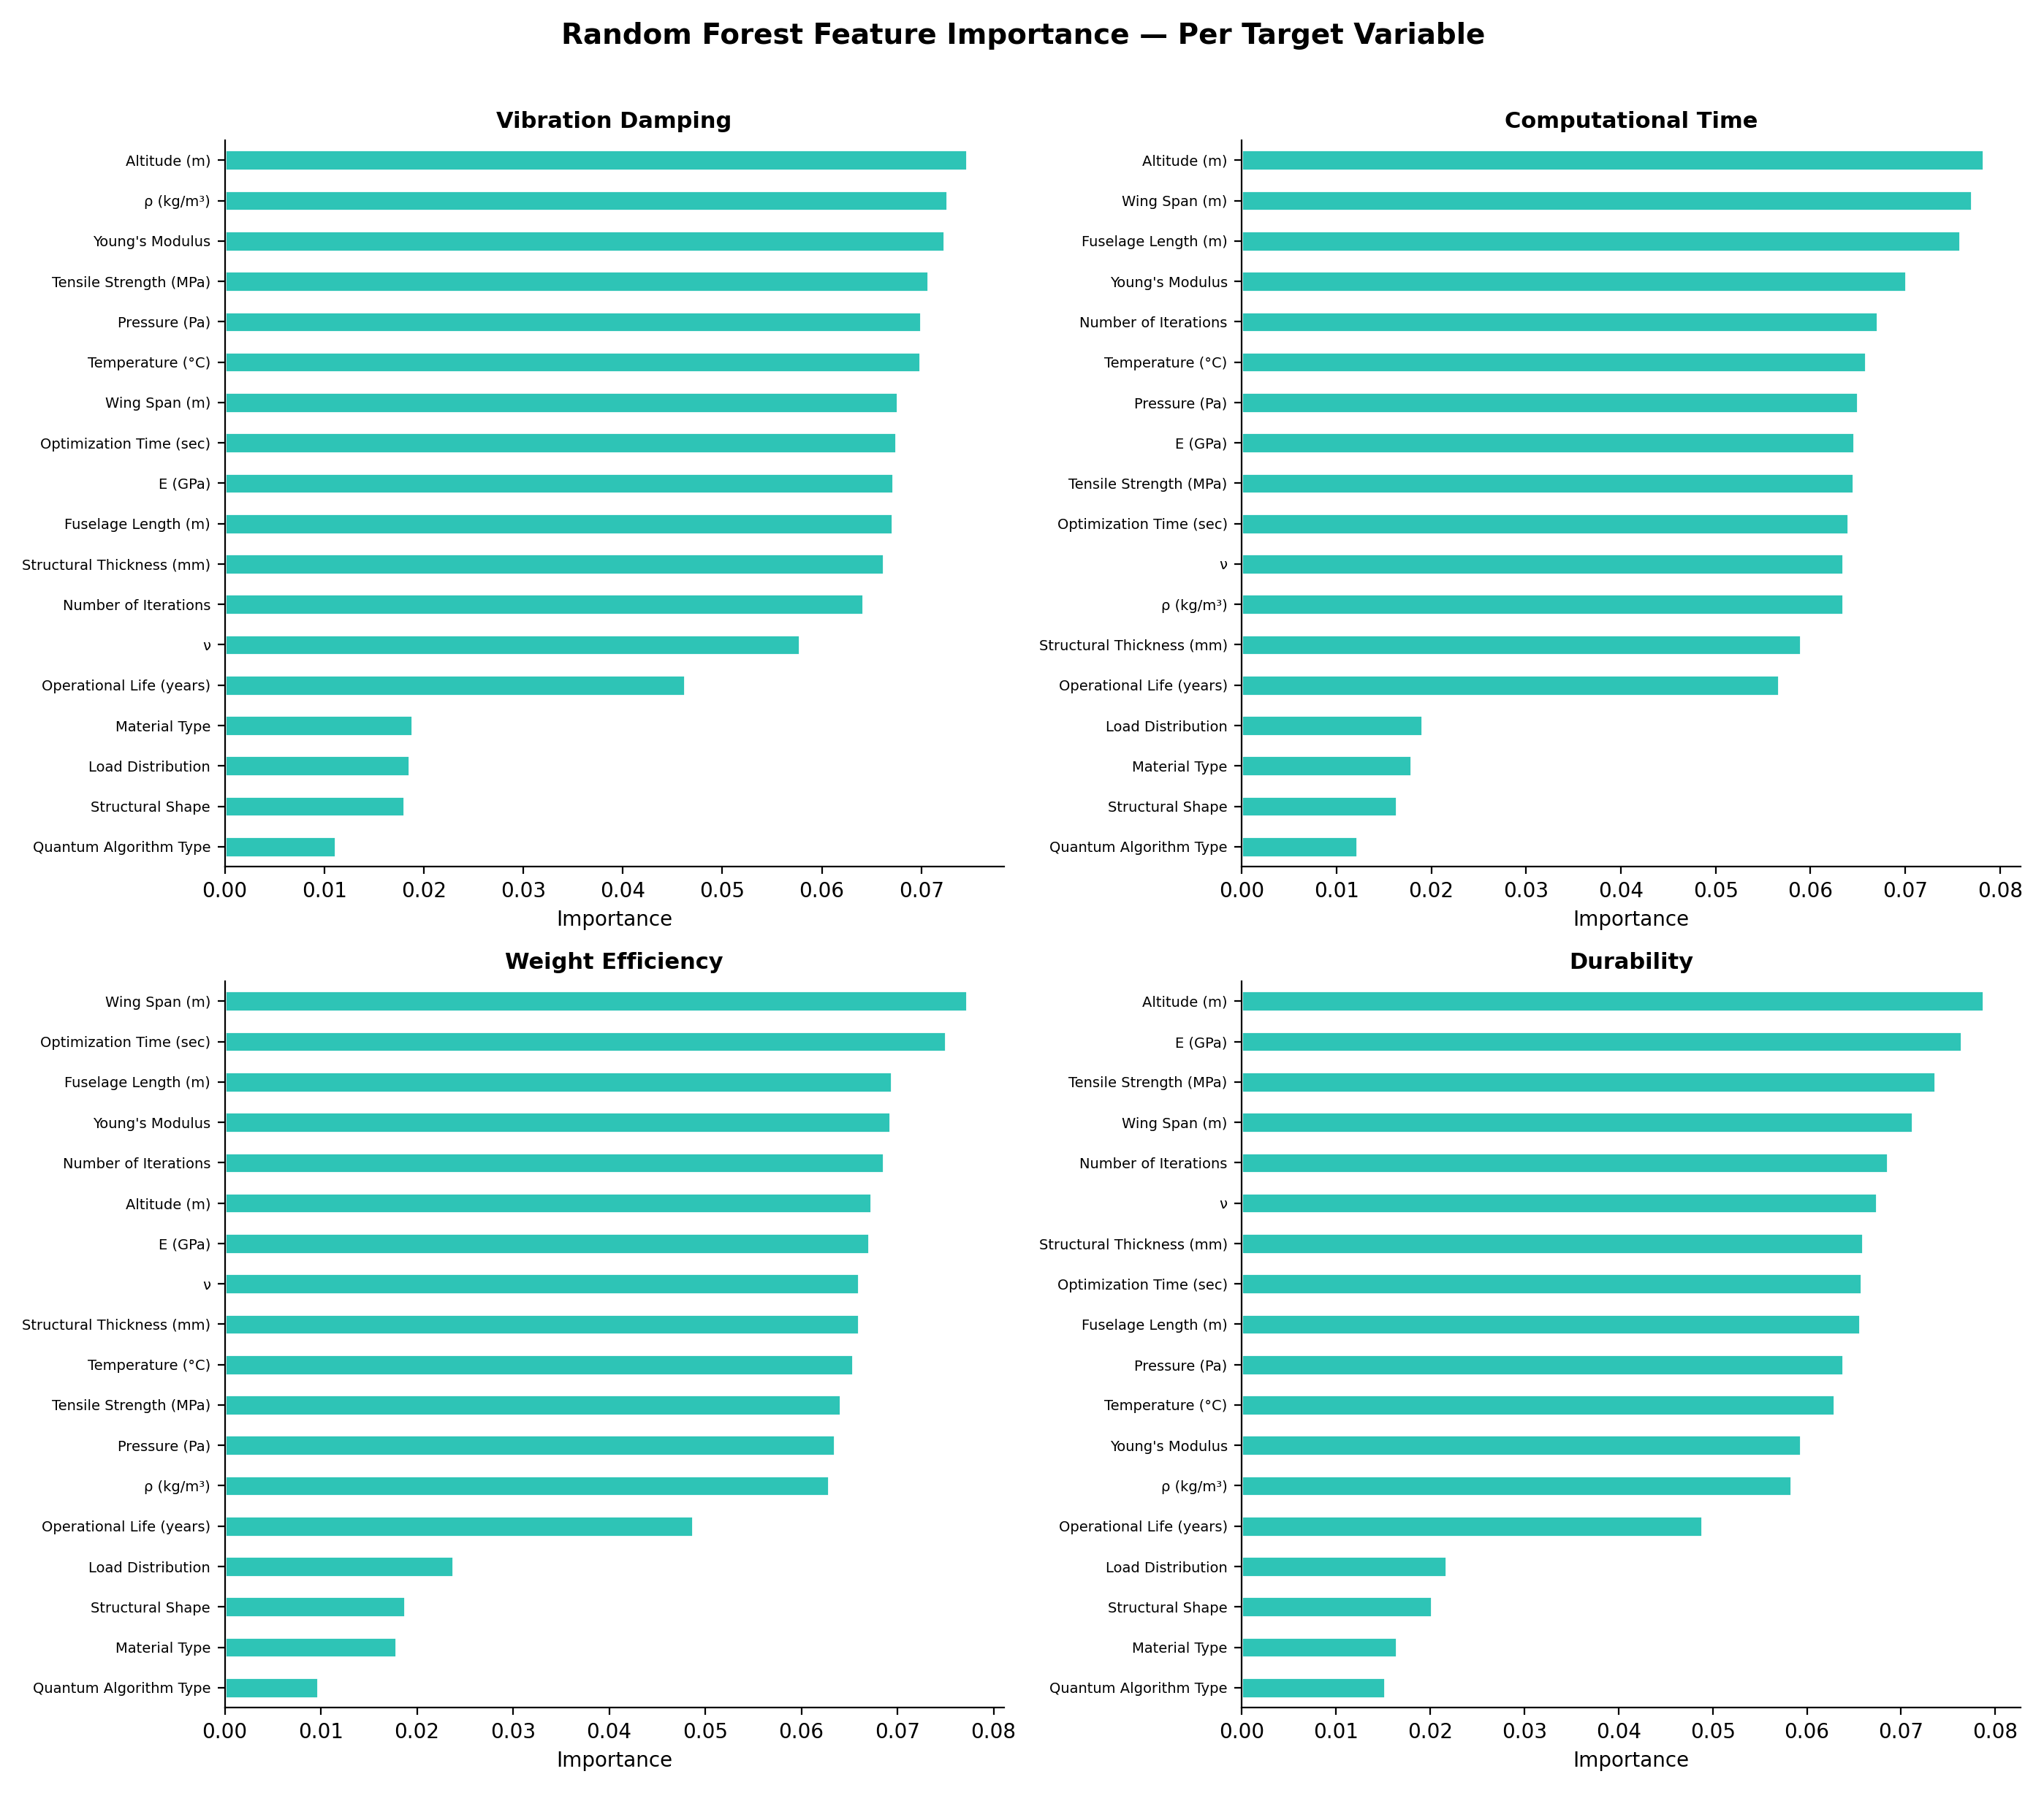
\includegraphics[width=\textwidth]{ch10_feature_importance_per_target}
\caption{Random Forest feature importance for each of the 4 target variables. No single feature dominates --- importance is distributed relatively uniformly across features.}
\label{fig:fi_per_target}
\end{figure}

\section{Feature Importance Heatmap}

\begin{figure}[H]
\centering
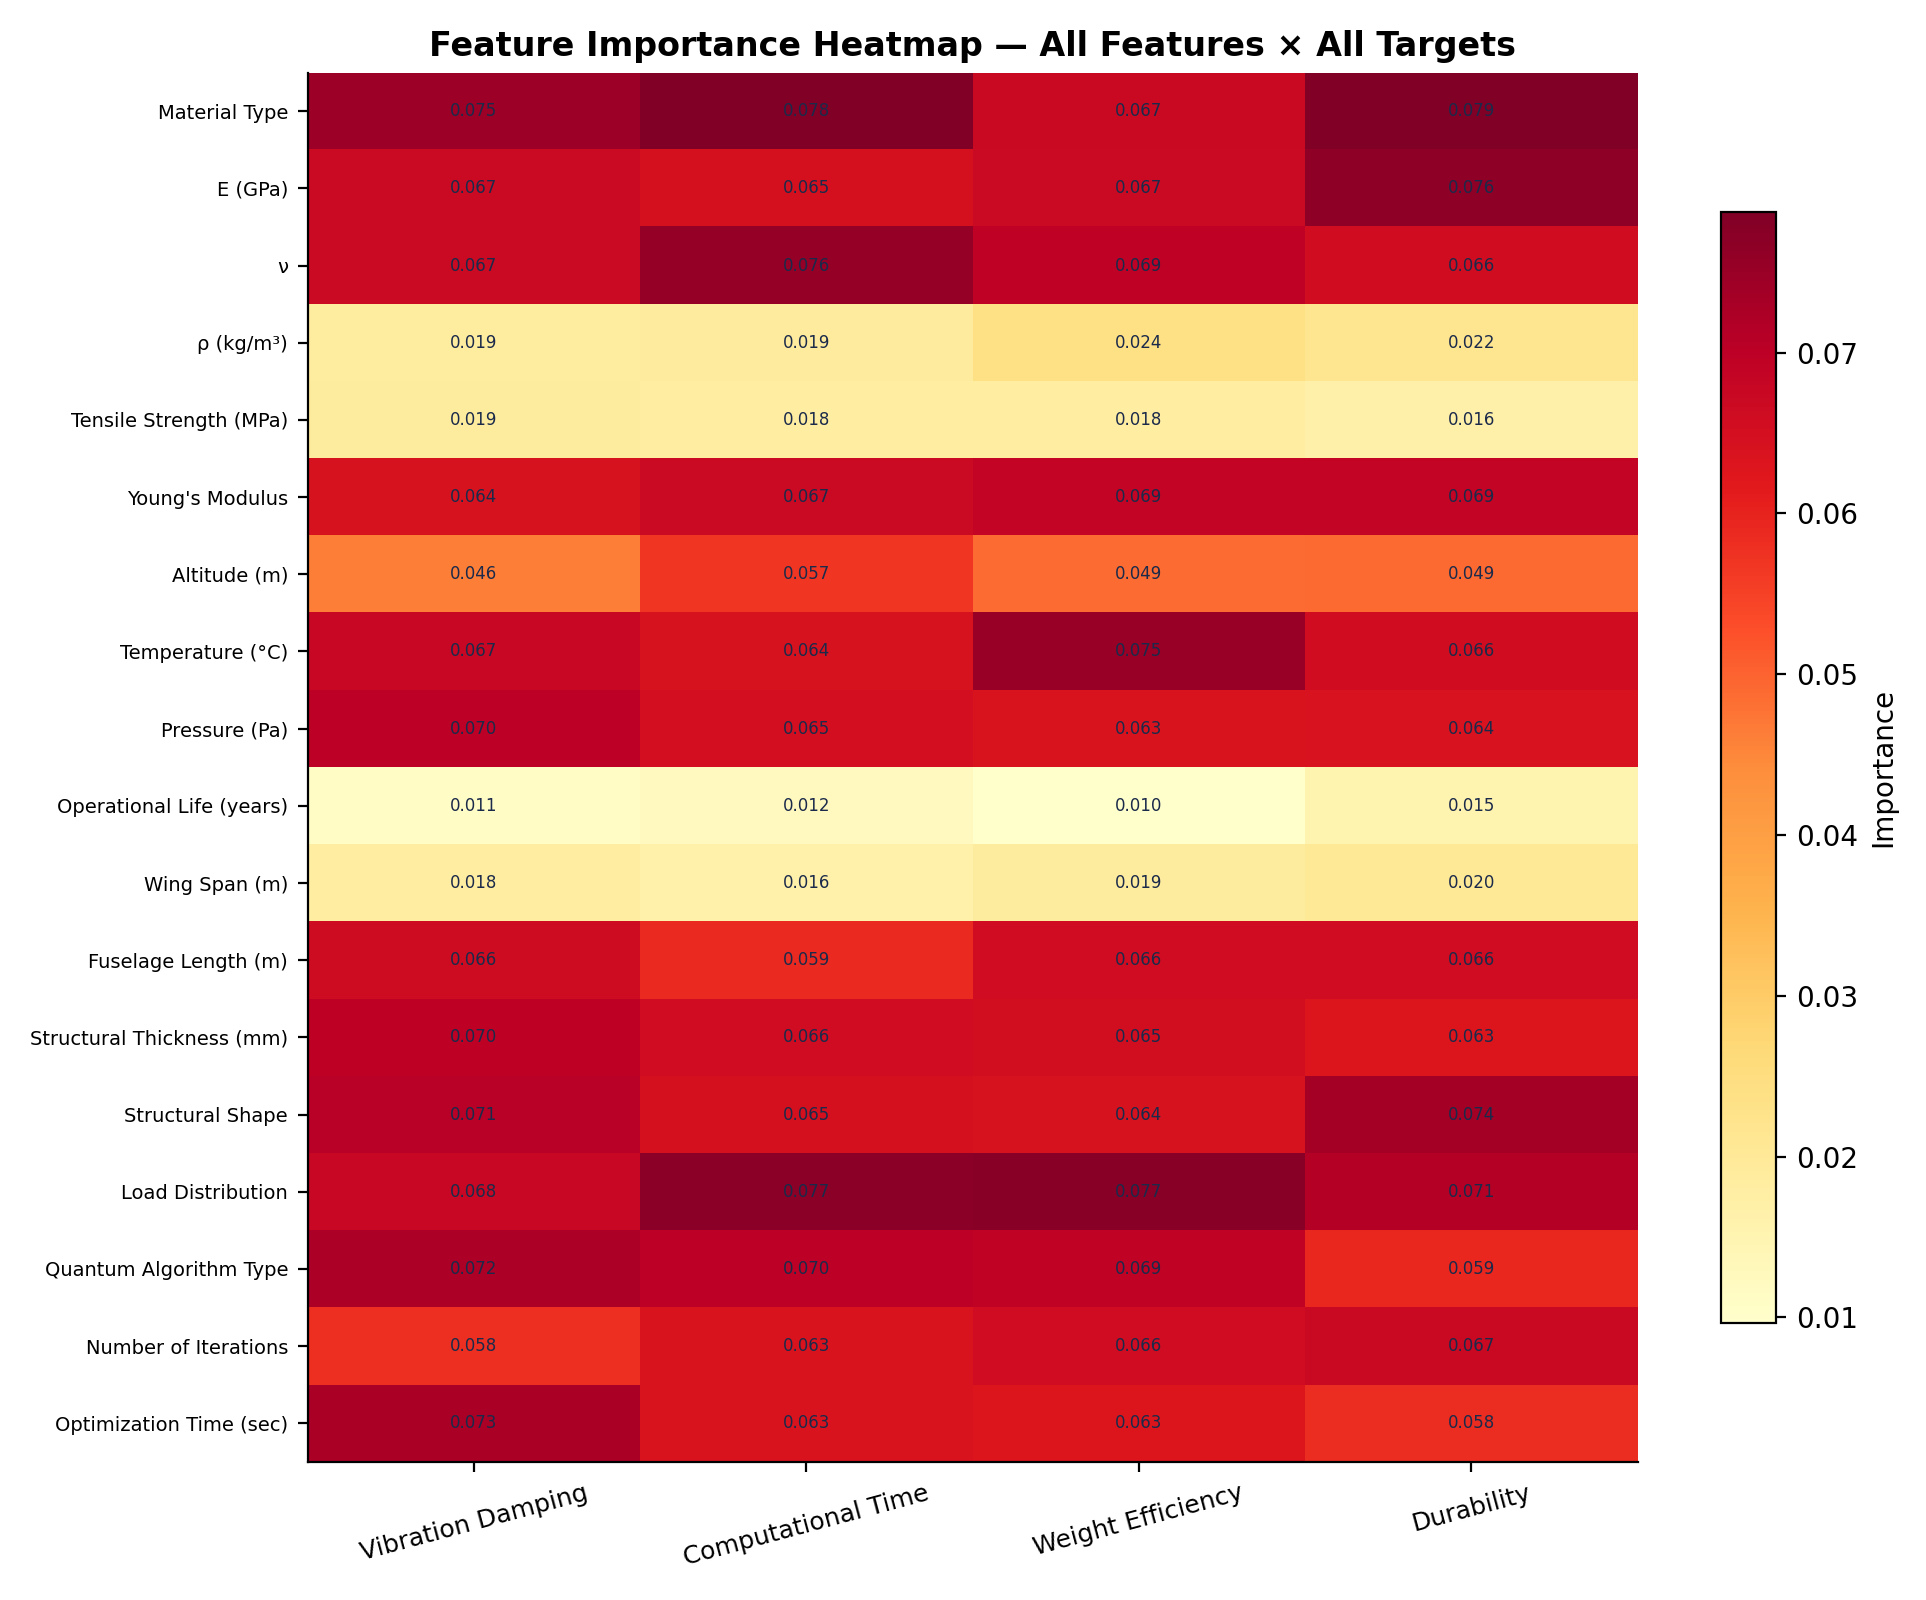
\includegraphics[width=0.85\textwidth]{ch10_importance_heatmap}
\caption{Feature importance heatmap across all targets. Warmer colors indicate higher importance. The diffuse importance pattern confirms that no small feature subset drives target outcomes.}
\label{fig:fi_heatmap}
\end{figure}

\begin{findingbox}
Feature importance is \textbf{uniformly distributed} across input features for all four targets. No single feature achieves importance $> 0.12$ for any target. This is consistent with:
\begin{itemize}[nosep]
\item Independently sampled features with no causal relationship to targets
\item Target assignments that are either random or based on complex non-linear interactions not captured by tree-based importance
\item A simulation design where target labels were assigned via a hidden rule involving all features simultaneously
\end{itemize}
\end{findingbox}

\begin{warningbox}
\textbf{Implication for synthetic generation:} Since no feature subset drives target outcomes, synthetic generators must preserve the \emph{entire} 22-dimensional joint distribution rather than focusing on a few key features. Feature selection or dimensionality reduction before generation would be inappropriate.
\end{warningbox}


% ══════════════════════════════════════════════════════════════════════════════
\chapter{Anomaly \& Outlier Analysis}
% ══════════════════════════════════════════════════════════════════════════════

Two complementary anomaly detection methods were applied to identify rows that deviate from the dominant data distribution.

\section{Detection Methods}

\begin{itemize}[nosep]
\item \textbf{Isolation Forest (IF):} Ensemble of isolation trees; anomalies are points that require fewer splits to isolate. Contamination threshold: 10\%.
\item \textbf{Local Outlier Factor (LOF):} Density-based method; anomalies are points in low-density neighborhoods relative to their neighbors. $k=20$ neighbors, contamination 10\%.
\end{itemize}

\begin{figure}[H]
\centering
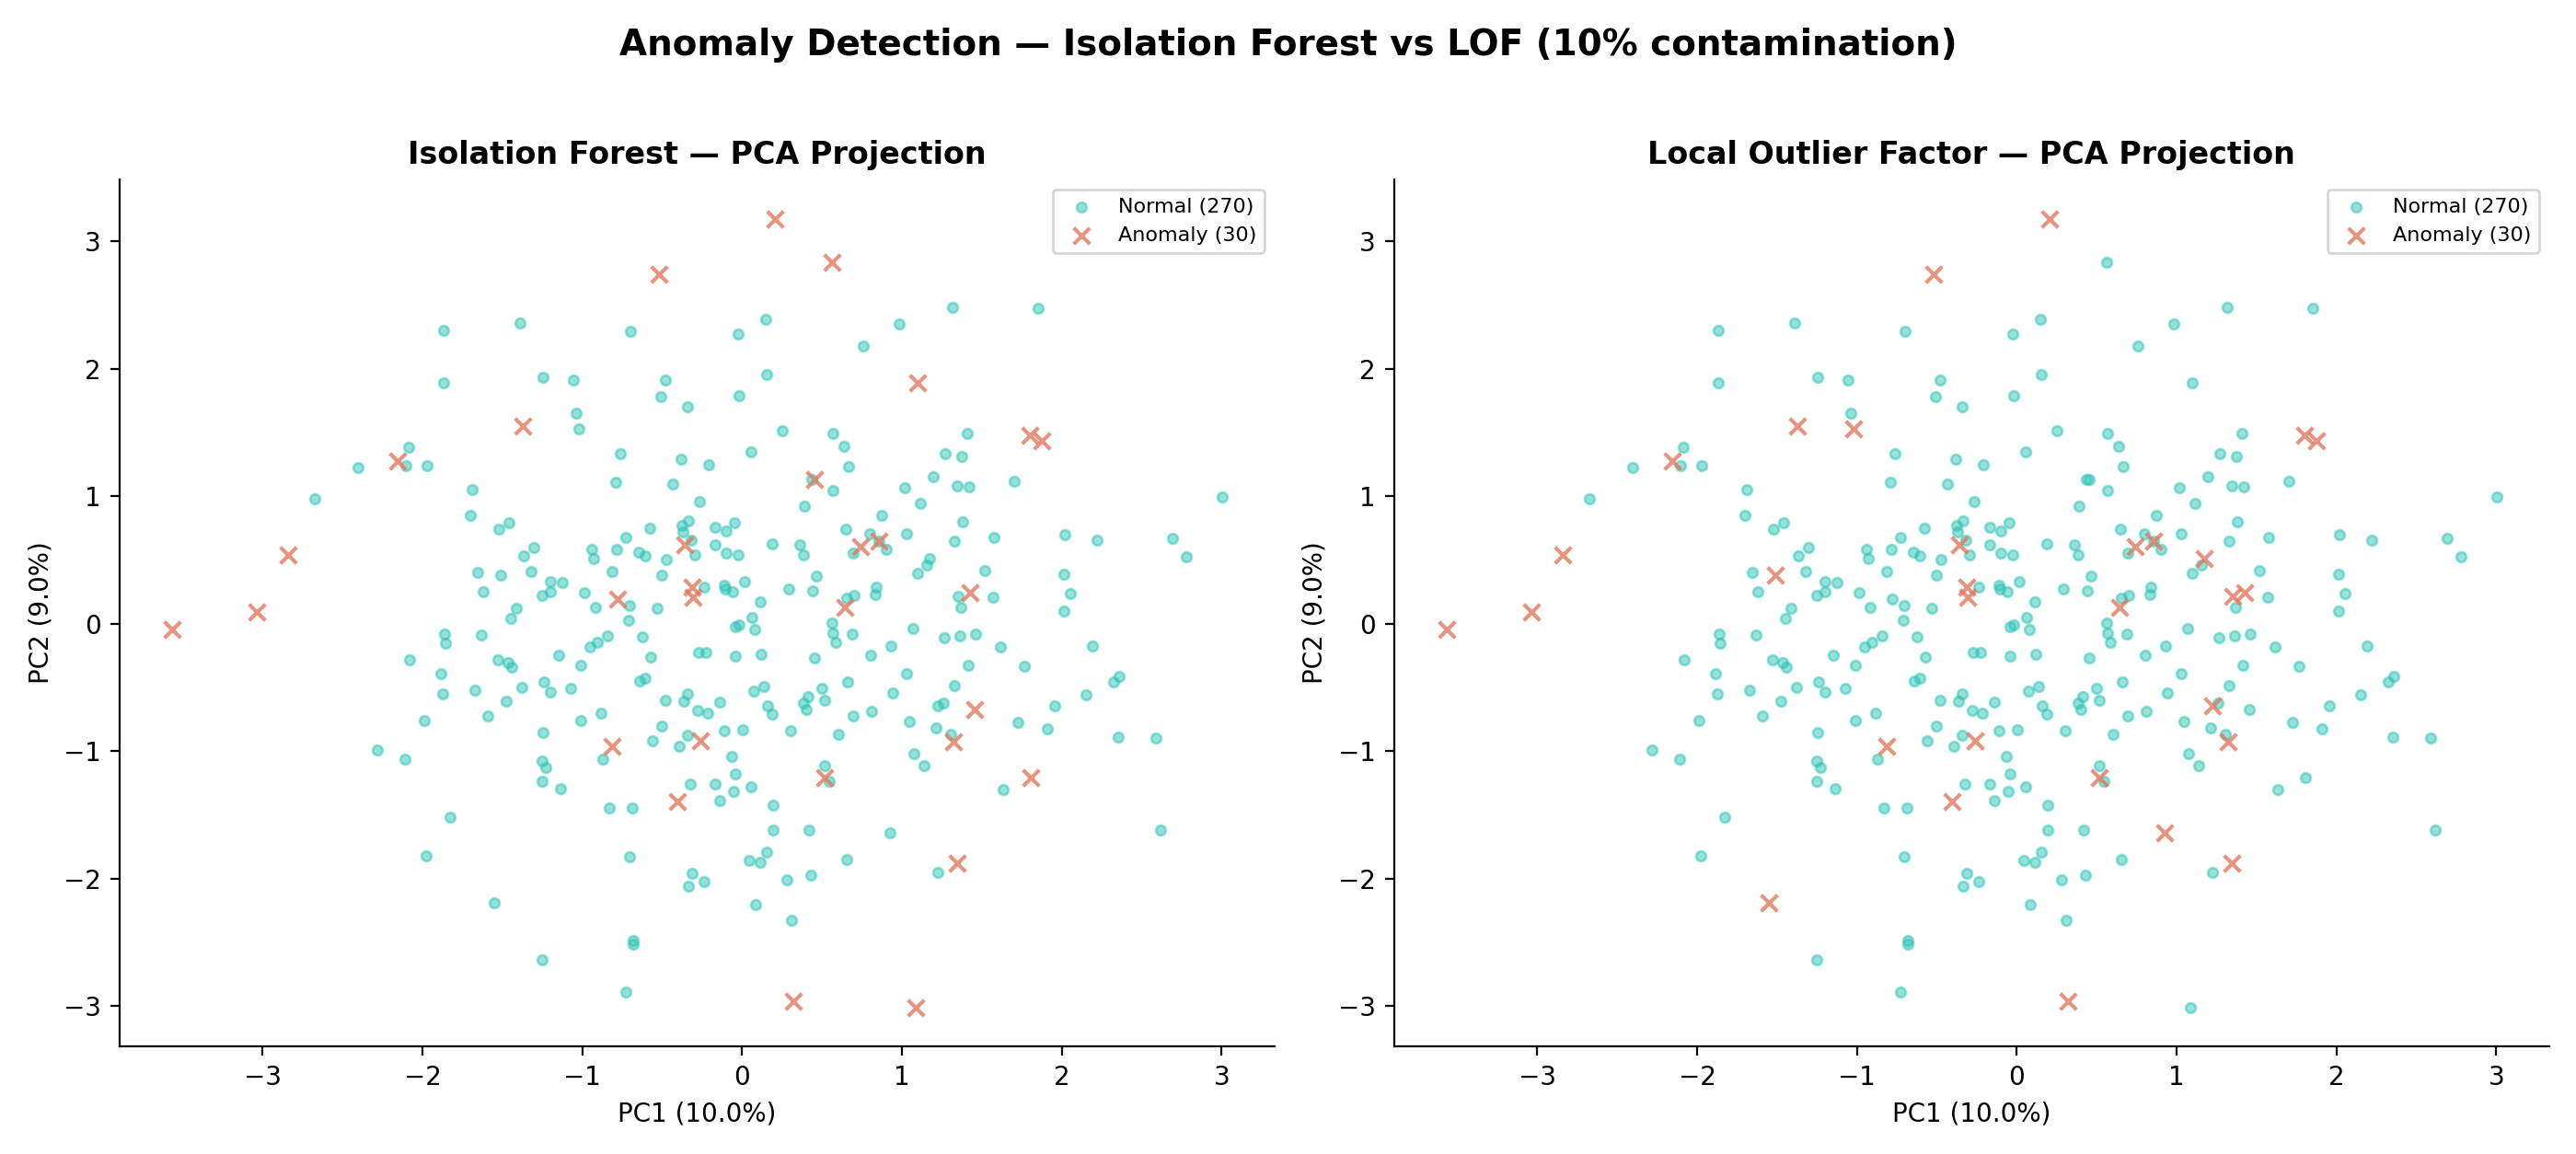
\includegraphics[width=\textwidth]{ch11_anomaly_pca}
\caption{Anomaly detection results projected onto the first two principal components. \textbf{Left:} Isolation Forest flags 30 anomalies (10\%). \textbf{Right:} LOF flags 30 anomalies (10\%). Anomalies are scattered throughout the space rather than forming distinct clusters.}
\label{fig:anomaly}
\end{figure}

\begin{findingbox}
Both IF and LOF detect anomalies \textbf{uniformly distributed throughout the feature space}, not concentrated in corners or boundaries. This is expected for uniformly-distributed data: the ``anomalies'' are simply points that happen to be slightly farther from their neighbors in the 14-dimensional space, not true structural outliers. The overlap between IF and LOF anomalies is moderate, further confirming the absence of a distinct outlier population.
\end{findingbox}

\section{Dimensionality Analysis}

\begin{figure}[H]
\centering
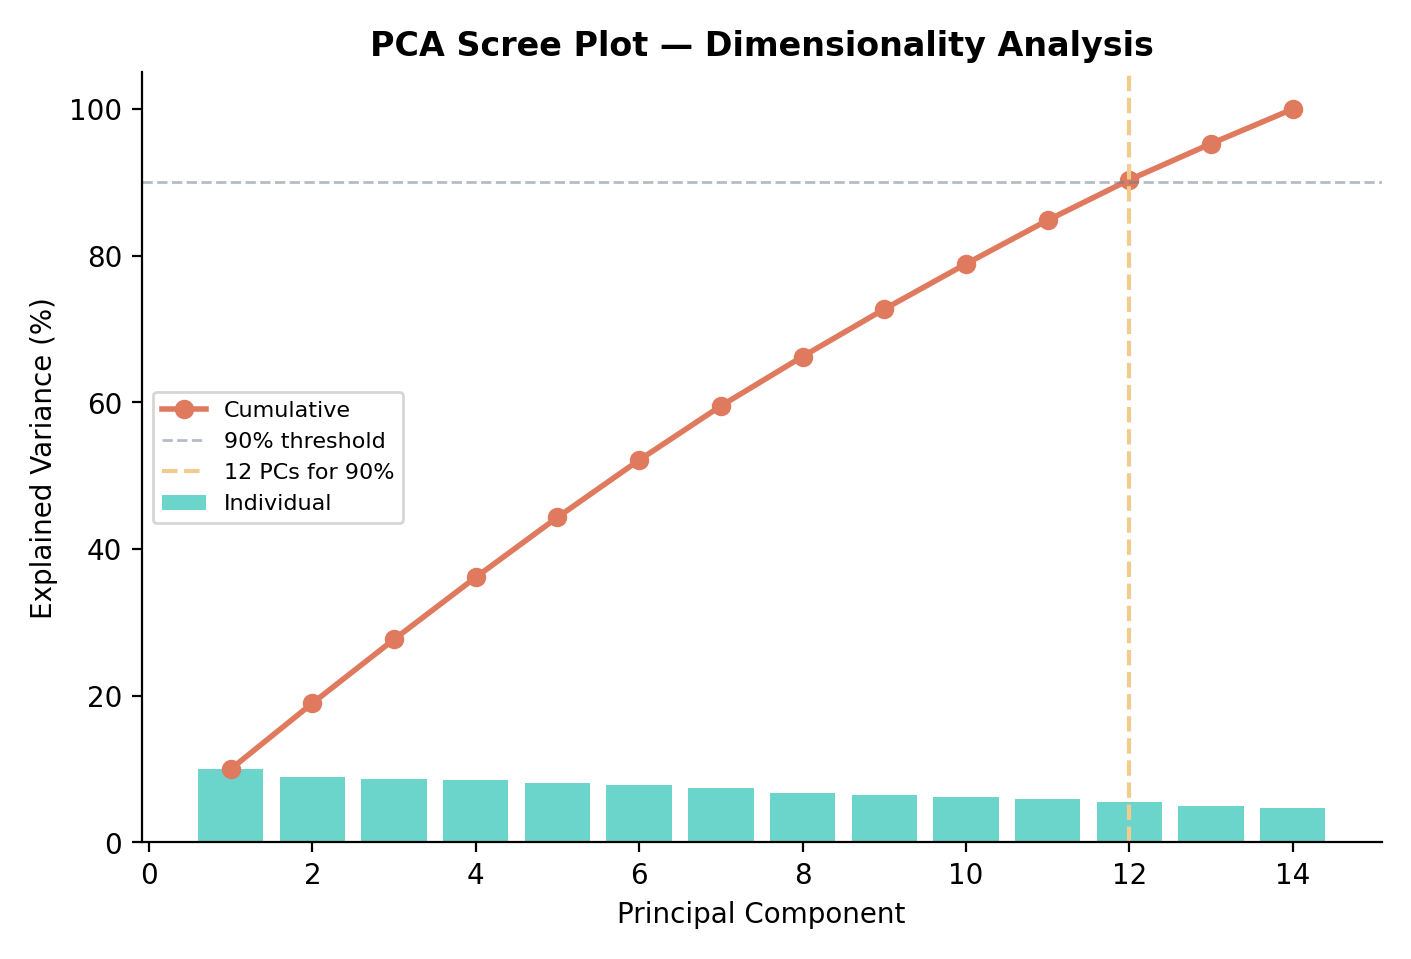
\includegraphics[width=0.75\textwidth]{ch11_pca_scree}
\caption{PCA scree plot. Variance is distributed approximately equally across components, consistent with orthogonal features. 13 components are needed to reach 90\% explained variance.}
\label{fig:scree}
\end{figure}

The PCA scree plot reveals that no small number of principal components captures the majority of variance. Each of the 14 numeric features contributes approximately $1/14 \approx 7.1\%$ of total variance, consistent with the near-zero correlation structure. This confirms that the dataset is \textbf{intrinsically 14-dimensional} --- there is no meaningful lower-dimensional manifold.

\section{t-SNE Projection}

\begin{figure}[H]
\centering
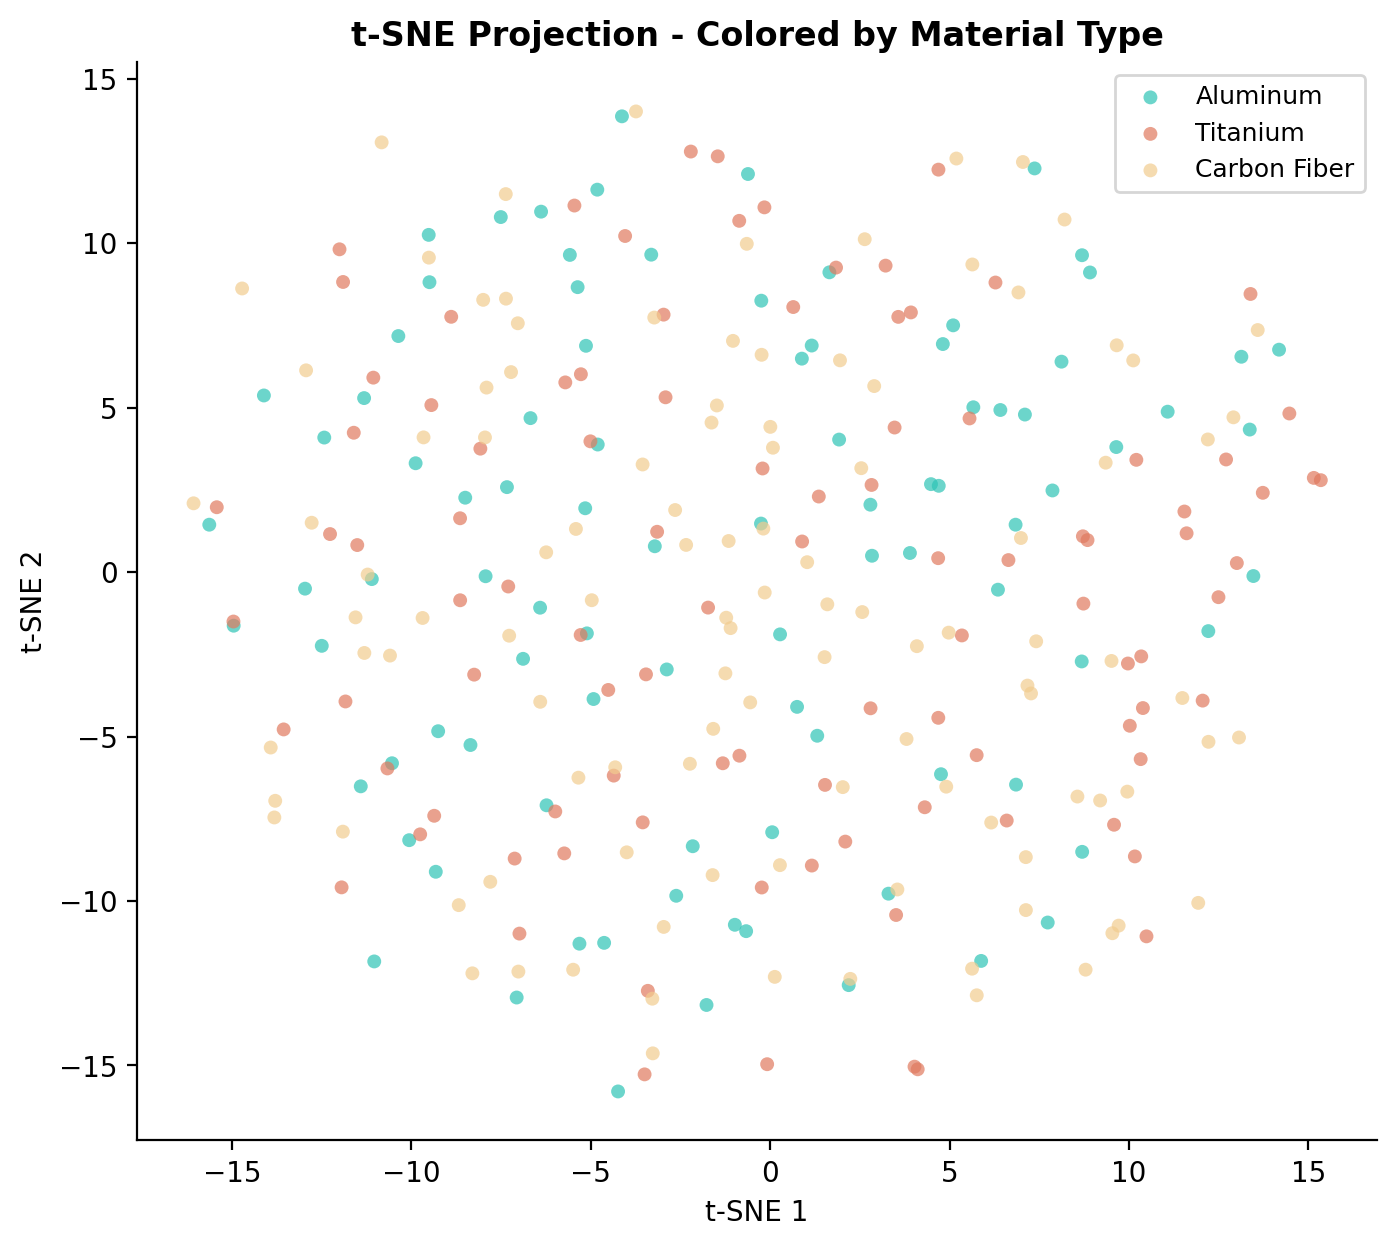
\includegraphics[width=0.7\textwidth]{ch11_tsne_material}
\caption{t-SNE projection (perplexity=30) colored by Material Type. The three materials show partial separation, driven primarily by the E (GPa) feature.}
\label{fig:tsne}
\end{figure}

The t-SNE visualization reveals that Material Type provides the \textbf{only visually identifiable clustering structure} in the dataset. The three material clusters overlap significantly, consistent with the fact that only E (GPa) differs meaningfully across materials.


% ══════════════════════════════════════════════════════════════════════════════
\chapter{Conclusions \& Red Lines}
% ══════════════════════════════════════════════════════════════════════════════

\section{Summary of Findings}

This analysis reveals a dataset with a distinctive statistical fingerprint: \textbf{uniformly distributed, mutually independent features} with \textbf{one dominant conditional structure} (Material Type $\rightarrow$ E). The key characteristics are:

\begin{enumerate}[leftmargin=*, itemsep=6pt]
\item \textbf{Simulation origin.} The dataset was generated by a computational simulation, not collected from field measurements. Evidence: perfect completeness, platykurtic distributions, near-zero correlations, ISA non-compliance, and independently sampled optimization parameters.

\item \textbf{Tri-modal E is the structural backbone.} The three-regime distribution of E (GPa), driven by Material Type, is the single most important distributional feature. Any synthetic generator that fails to reproduce this tri-modal structure produces physically implausible data.

\item \textbf{Feature independence simplifies generation but complicates validation.} With near-zero correlations, correlation-based fidelity metrics (Pearson difference, correlation Frobenius norm) will trivially pass for any generator. Marginal distribution matching (KS test per feature) is the decisive quality gate.

\item \textbf{Targets are independent of each other and weakly predicted by features.} No feature subset drives target outcomes. Multi-target prediction requires models that capture the full joint distribution.

\item \textbf{No true outliers exist.} The data fills its 14-dimensional hypercube approximately uniformly. Anomaly detectors flag boundary points, not structural deviants.
\end{enumerate}

\section{Red Lines for Synthetic Data Generation}

\begin{warningbox}
The following constraints must be respected by any synthetic data generator:
\begin{enumerate}[nosep]
\item \textbf{E (GPa) must be tri-modal.} Generators that apply global normalization (MinMax, Standard) will collapse the three material modes. Use per-mode normalization (e.g., BGM).
\item \textbf{Categorical levels must be preserved exactly.} All 8 categorical features have fixed levels (2 or 3 each). No novel levels should appear in synthetic data.
\item \textbf{Numeric ranges must be preserved.} Each feature has strict physical bounds. Synthetic values outside these bounds are invalid.
\item \textbf{Do not enforce ISA relationships.} Temperature and Pressure are independent of Altitude in this dataset.
\item \textbf{Preserve the uniform marginals.} Near-zero skewness and platykurtic shape are defining properties.
\item \textbf{22 columns, zero nulls.} Schema must be preserved exactly.
\end{enumerate}
\end{warningbox}

\section{Recommended Validation Protocol}

Based on this analysis, we recommend the following tiered validation for synthetic datasets:

\begin{table}[H]
\centering
\caption{Recommended validation tiers.}
\begin{tabular}{clp{8cm}}
\toprule
\textbf{Tier} & \textbf{Gate} & \textbf{Criteria} \\
\midrule
1 & Schema & 22 columns, zero nulls, correct dtypes, exact categorical levels, exact numeric bounds, $\geq 300$ rows \\
2 & Distributional & KS test per numeric feature ($\geq 12/14$ pass at $\alpha=0.05$), KL divergence $< 0.1$, categorical frequency match \\
3 & Structural & Correlation Frobenius norm $< 0.5$, E tri-modality preserved, material-conditioned E ranges correct \\
4 & Utility & TSTR macro-F1 $\geq 0.25$ across all 4 targets, discriminator AUC $< 0.70$ \\
\bottomrule
\end{tabular}
\end{table}


% ── Appendix ──────────────────────────────────────────────────────────────────
\appendix
\chapter{Statistical Test Reference}

\section{Shapiro--Wilk Normality Test}
All 14 numeric features reject the null hypothesis of normality at $\alpha = 0.05$ ($p < 10^{-5}$ for all). The test statistic $W$ ranges from 0.935 (Altitude) to 0.968 ($\nu$).

\section{Kolmogorov--Smirnov Test}
The two-sample KS test is used throughout this project to compare synthetic vs.\ real distributions. The null hypothesis is that both samples are drawn from the same continuous distribution. We use $\alpha = 0.05$.

\section{ANOVA Assumptions}
One-way ANOVA assumes normality and homoscedasticity. Given the non-normal distributions, we verified results with the non-parametric Kruskal--Wallis test, which yielded consistent conclusions.

\end{document}
